%!TEX root = ../main.tex
\chapter{Timing study of hadron showers}
\label{chap:TimingPions}

In this section, the pion data collected is compared to \geant v10.1 simulations using different hadronic models as explained in chapter \ref{chap:G4Simulation}.

\section{Hadronic shower timing}

The table \ref{table:pion_runs} summarizes the runs and datasets used for the pion analysis. The calibration is applied to pion data directly after the selection. The pion selection is applied as described in section \ref{sec:pionsel}. The table shows that more 80\% of the events pass the trigger selection.

{
\renewcommand{\arraystretch}{1.5}
\begin{table}[htb!]
	\centering
	\caption{Table with the statistic before and after selection used for the pion dataset.}
	\label{table:pion_runs}
	%\resizebox{0.9\textwidth}{!}{%
	\begin{tabularx}{\textwidth}{>{\hsize=1.1\hsize}Xlllll}
		\hline
		Runs & Energy & Particle Type & Events (3 T0s) & Events (sel.) & $\frac{\text{N$_{sel.}$}}{\text{N$_{raw}$}}$ \\
		\hline
		24306-24317 \newline 24381-24397 & 10 GeV & $\pi^-$ & 425517 & 349012 & 82\% \\
		\hline
		24578-24612 & 50 GeV & $\pi^-$ & 1183790 & 1007889 & 85.1\% \\
		\hline
		24339-24342 & 70 GeV & $\pi^-$ & 142813 & 122376 & 85.7\% \\
		\hline
		24223-24238 \newline 24273-24287 \newline 24331-24336 \newline 24358-24364 & 90 GeV & $\pi^-$ & 466927 & 395884 & 84.8\% \\
		\hline
	\end{tabularx}
	%}
\end{table}
}

Inside a hadronic shower, absorber materials with a high atomic number Z, therefore containing a high number of neutrons, are expected to release a high number of evaporation neutrons. These neutrons then will deposit energy by two different mechanisms with different time scales relative to the first hard interaction.

First, the elastic scattering of neutrons in the active material especially with high hydrogen content will play a role at a few nanoseconds to tens of nanoseconds time scale, whereas neutron capture in the absorber material at the interface with the active material will contribute to several hundred or thousands of nanoseconds timescale due to the relatively long time of flight of thermal neutrons and the lifetime of such atomic states. Thus it is expected that hadronic shower will present an increase in the late component compared to muons or electrons.

\begin{figure}[htbp!]
	\centering
	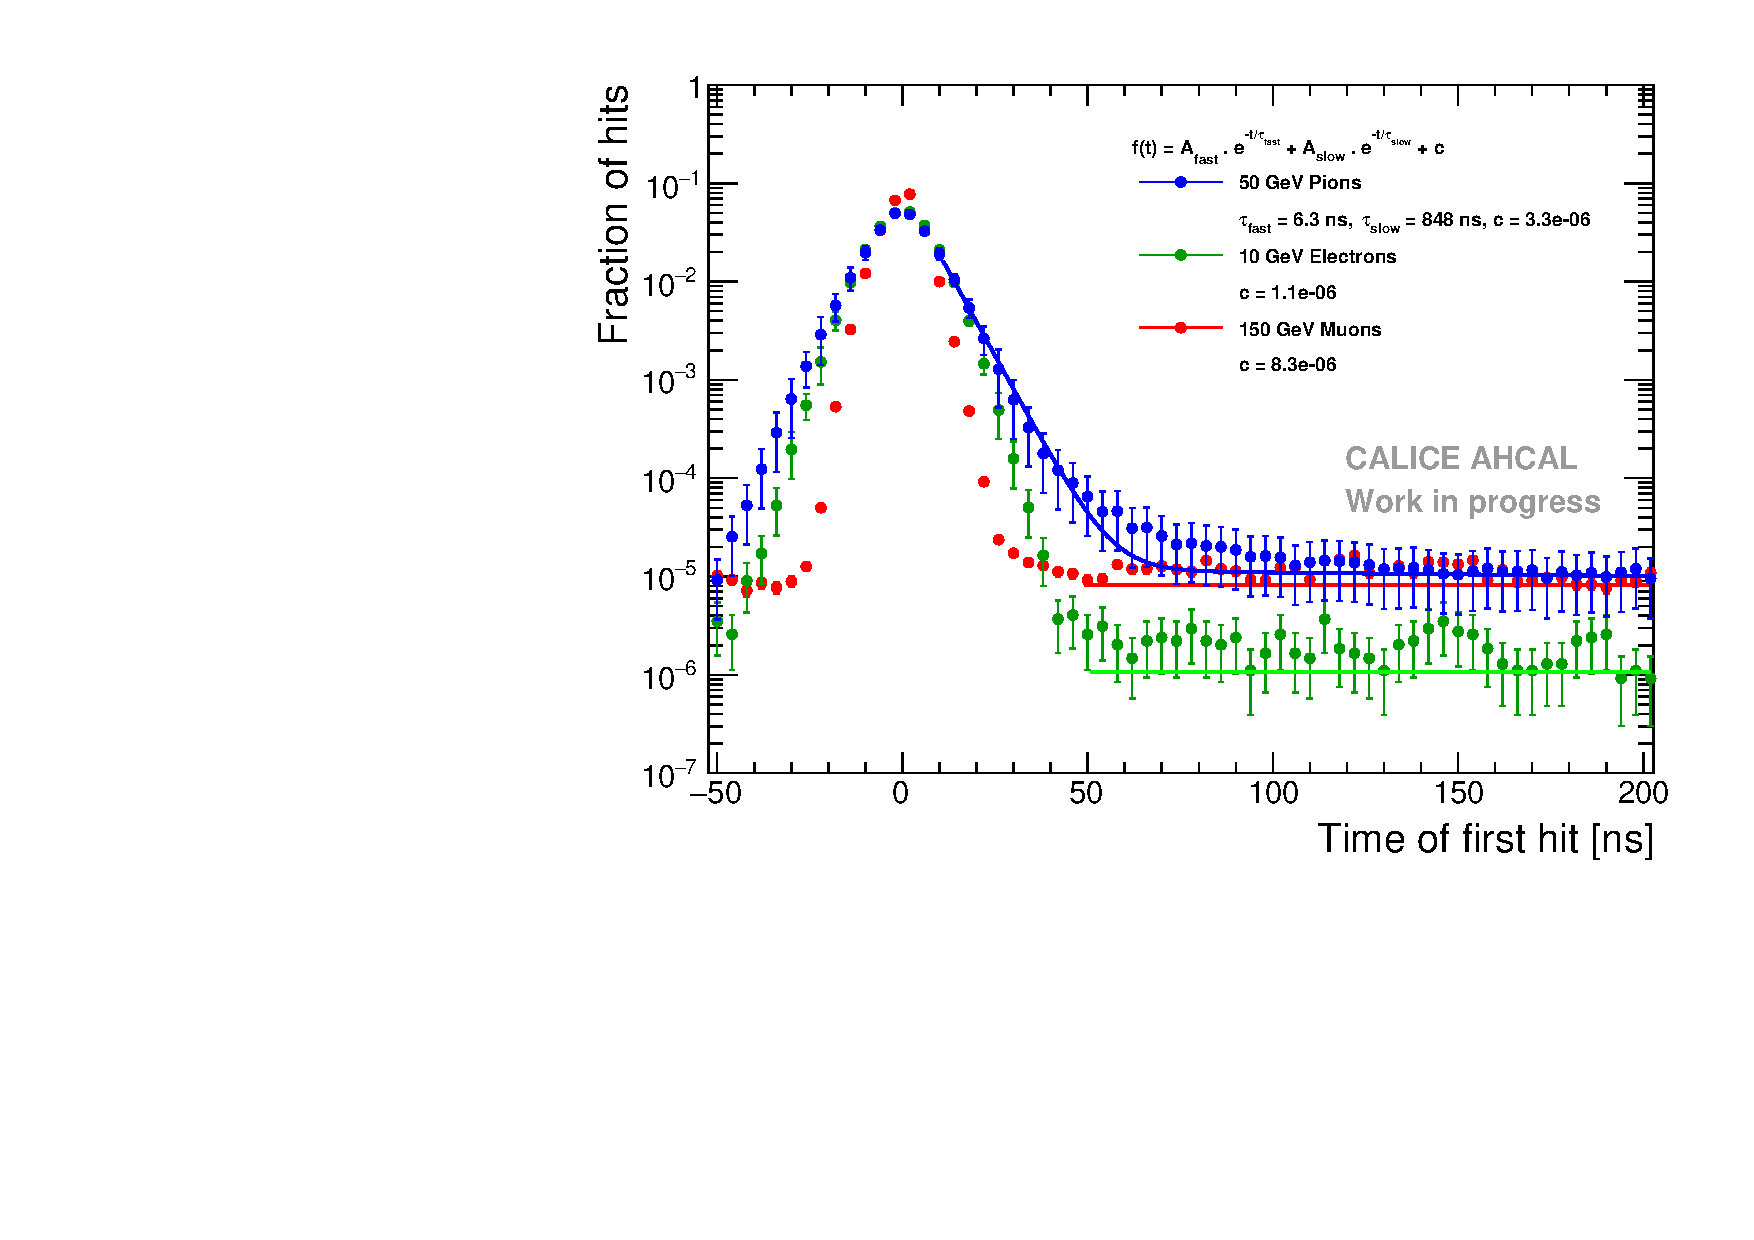
\includegraphics[width=0.7\textwidth]{../Thesis_Plots/Timing/Pions/Plots/Timing_dNdt_Comparison.pdf}
	\caption{Time of first hit for muons, electrons and pions in steel absorber in a range of -50 to 200 ns. The histograms are normalized to the number of events. The lines represent the fit to the data as explained in the text.}
	\label{fig:dNdt_Comparison}
\end{figure}

The figure \ref{fig:dNdt_Comparison} shows the time of first hit for muons, 10 GeV electrons and 50 GeV pions. Muon's and electron's energy depositions are instantaneous within a certain time window centered around $t=0$ ns (determined by the intrinsic time resolution of the detector). Some isolated hits are present in the tails most likely caused by SiPM thermal noise. This gives an idea of the noise level as well as the rejection of noise in the analysis. One can remark that the noise level in electron data is lower than in the muon data. The reason is not clear. It may come from the difference in beam rate and also the difference of the detector configuration of the thresholds.

For muons, around 2\% of hits are later than 50 ns compared to the core of the distribution between -50 and 50 ns. For electrons, only 0.37\% of hits are later than 50 ns. For hadron showers, the situation is different. In this case, about 1.5\% of hits are after 50 ns. Moreover, the pion data presents a higher tail between 30 to 50 ns than in the electron data. In order to characterize the distribution, a similar model of the sum of two exponentials and a constant as the T3B experiment \cite{Simon2013} is applied following the equation \ref{eq:dNdt_eq}:

\begin{equation} \label{eq:dNdt_eq}
	\frac{1}{N}\frac{dN}{dt} = A_{fast} \times e^{-\frac{t}{\tau_{fast}}} + A_{slow} \times e^{-\frac{t}{\tau_{slow}}} + c
\end{equation}

where $A_{fast}, \tau_{fast}$ and $A_{slow}, \tau_{slow}$ are the amplitudes and decays times of the modeled fast and slow component of the hadronic shower. Since the fit is performed on several orders of magnitudes, the same method is used that T3B has applied for fitting. It is done in two steps. First, the slow component is fitted between 90 ns and \SI{2}{\micro\second}. Then fixing the parameters of the slow component, the fast component is fitted between 10 ns to \SI{2}{\micro\second}.
With this procedure, a fast component of $7.04 \pm 0.59$ ns and a slow component of $826 \pm 183$ ns are fitted. The fast component is in the same order of magnitude as given by T3B of 8 ns and interpreted by the evaporation neutrons energy depositions in the active medium. But due to the time resolution of the AHCAL being in the same order of magnitude, it is difficult to confirm this origin. On the other hand, the slow component is very different than in T3B (around 80 ns in steel). This may be due to the contribution of SiPM noise which reduces the sensitivity to this slow component in the shower. One can also remark that this model may be incomplete as the fitting function does match well the data in the transition region of 50 to 100 ns similar to the T3B data. The table \ref{table:dNdt_fit} sums up the fitted results.

\begin{table}[htb!]
	\centering
	\caption{Summary of the fit results in figure \ref{fig:dNdt_Comparison}.}
	\label{table:dNdt_fit}
	\begin{tabular}{@{} lccc @{}}
		\hline
		Parameter & Muon & Electron & Pion \\
		\hline
		$\tau_{fast}$ [ns] & - & - & $7.04 \pm 0.59$ \\
		$\tau_{slow}$ [ns] & - & - & $826 \pm 183$ \\
		$c$ & $(7.91 \pm 0.09) \times 10^{-6}$ & $(1.20 \pm 0.02) \times 10^{-6}$ & $(3.38 \pm 0.56) \times 10^{-6}$ \\
		\hline
	\end{tabular}
\end{table}

The energy dependence of the timing of hits has been studied in a second step as shown in figure \ref{fig:Energy_Comparison}. It shows the mean time of first hit taken between [-50, 200] ns as function of the hit energy for muon, electron and pion beams. For muons and electrons, no dependence on energy is observed as expected as all hits are prompt. For pions, the situation is different. A delay of 2-3 ns at 0.5 MIP is observed and decreases down to 0-1 ns above 1 MIP. For higher pion energies than 10 GeV, a dip in the distribution can be observed between 0.5 and 1.5 MIP. This effect is most likely due to an over-correction of the data with the number of triggered channels in a chip. In principle, it should follow the same shape as for 10 GeV pions as there should be no dependency on beam energy. Moreover, this effect is small especially given the large systematics uncertainties.

\begin{figure}[htbp!]
	\centering
	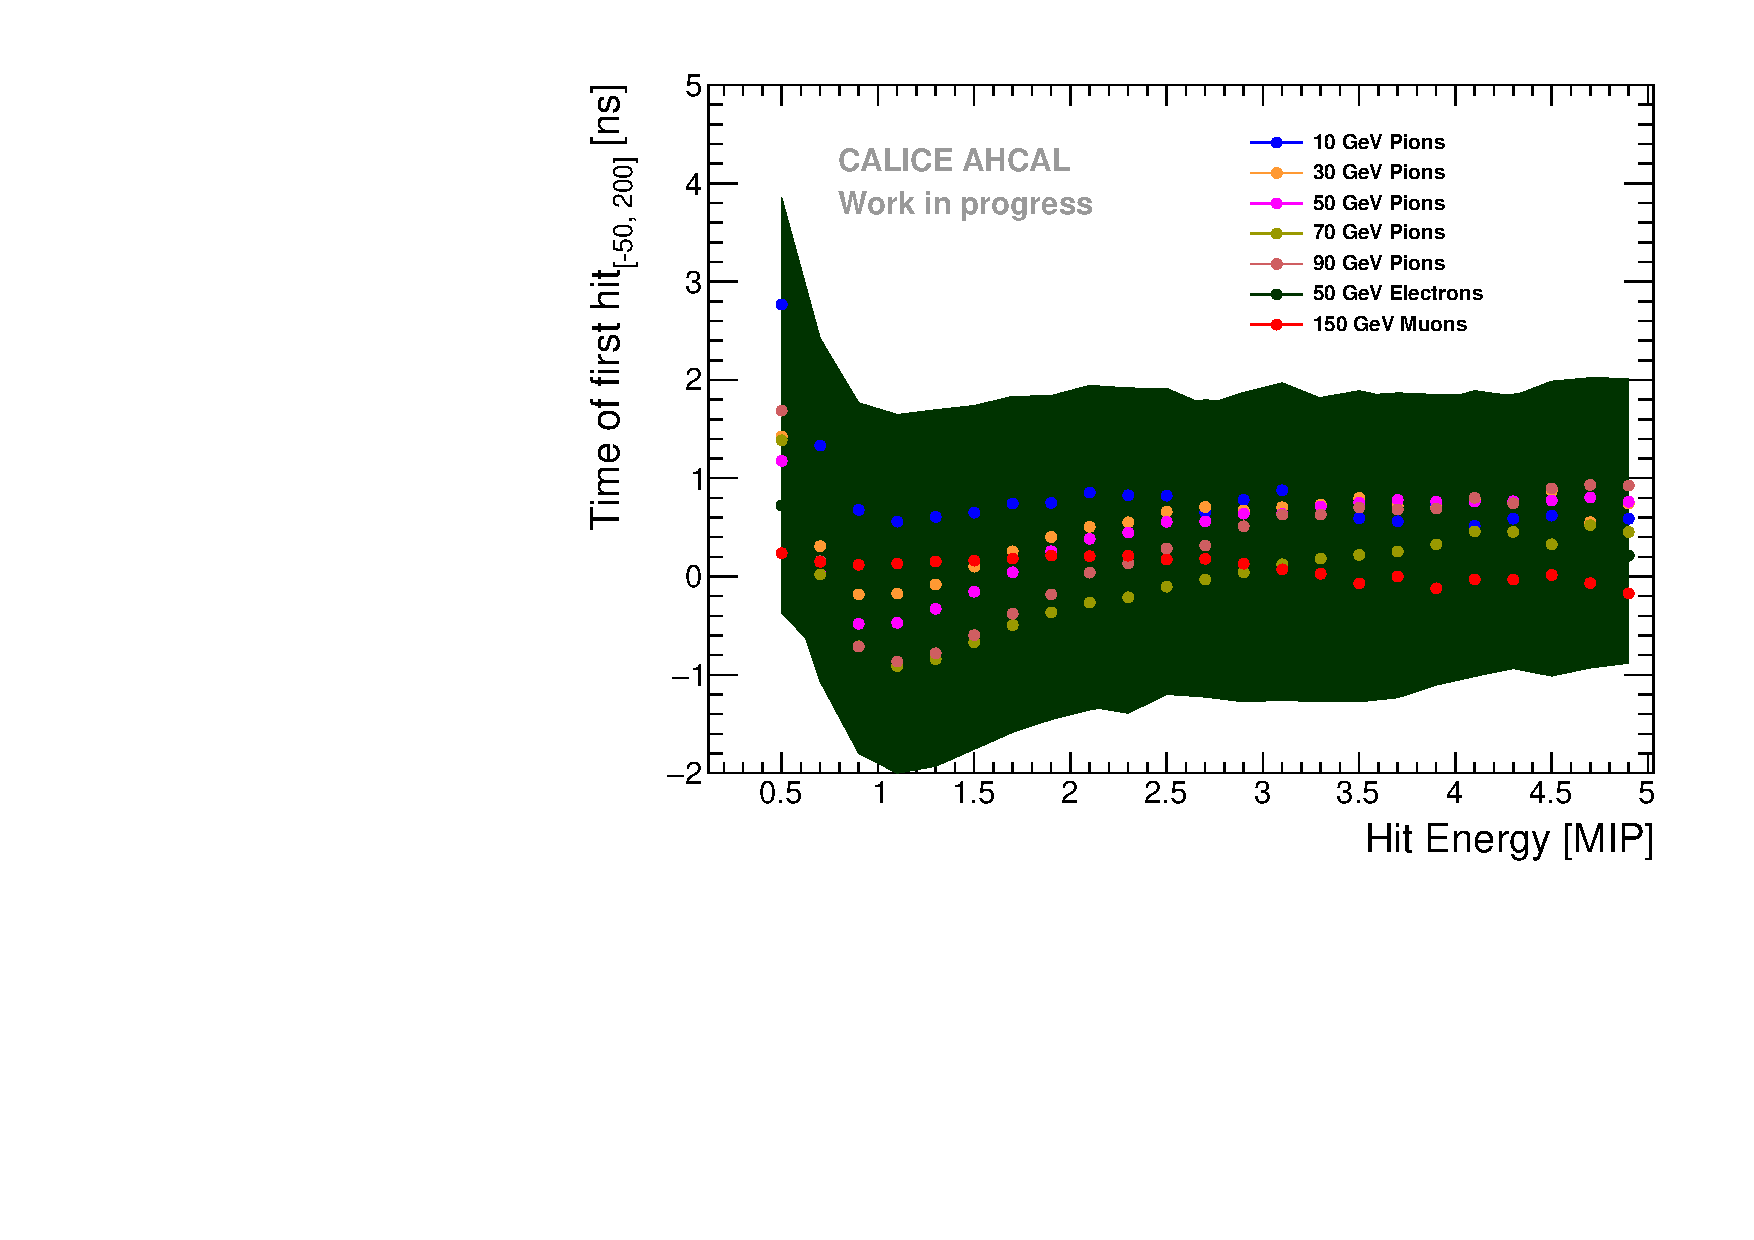
\includegraphics[width=0.7\textwidth]{../Thesis_Plots/Timing/Pions/Plots/Timing_Energy_Comparison_ShortAsymRange.pdf}
	\caption{Time of first hit as function of the hit energy for muons, electrons and pions in steel absorber in a range of -50 to 200 ns. The bands represent the systematic uncertainty.}
	\label{fig:Energy_Comparison}
\end{figure}

This figure demonstrates that low energy hits are responsible for delayed deposition most likely by low energy neutron from capture and spallation processes. Higher energy deposits occur mostly in the prompt part of the hadron shower. In a next step, the data is compared to simulations.

The figure \ref{fig:dNdt_SimData_Comparison} shows the time distribution of first hits compared with three different physics lists for pion beams ranging from 10 to 90 GeV. For the core of the distribution under 50 ns, generally, all physics lists describe relatively well the distribution within systematics. From 10 to 50 GeV, QGSP\_BERT\_HP reproduces well the distribution. Above 50 GeV, the late tail is well described by the distribution but between 50 and 100 ns is not well reproduced and under-estimated. QBBC tends to over-estimate the late tail by around a factor 2. This somehow contradicts the observations made in the T3B experiment were QBBC agreed well with the time distribution for pions of 60 GeV. It may be related to the use of different \geant versions as T3B used \geant v9.4p03. For all distributions, QGSP\_BERT over-estimates the tail of the distribution by around a factor 10.

\begin{figure}[htbp!]
	\begin{subfigure}[t]{0.5\textwidth}
		\centering
		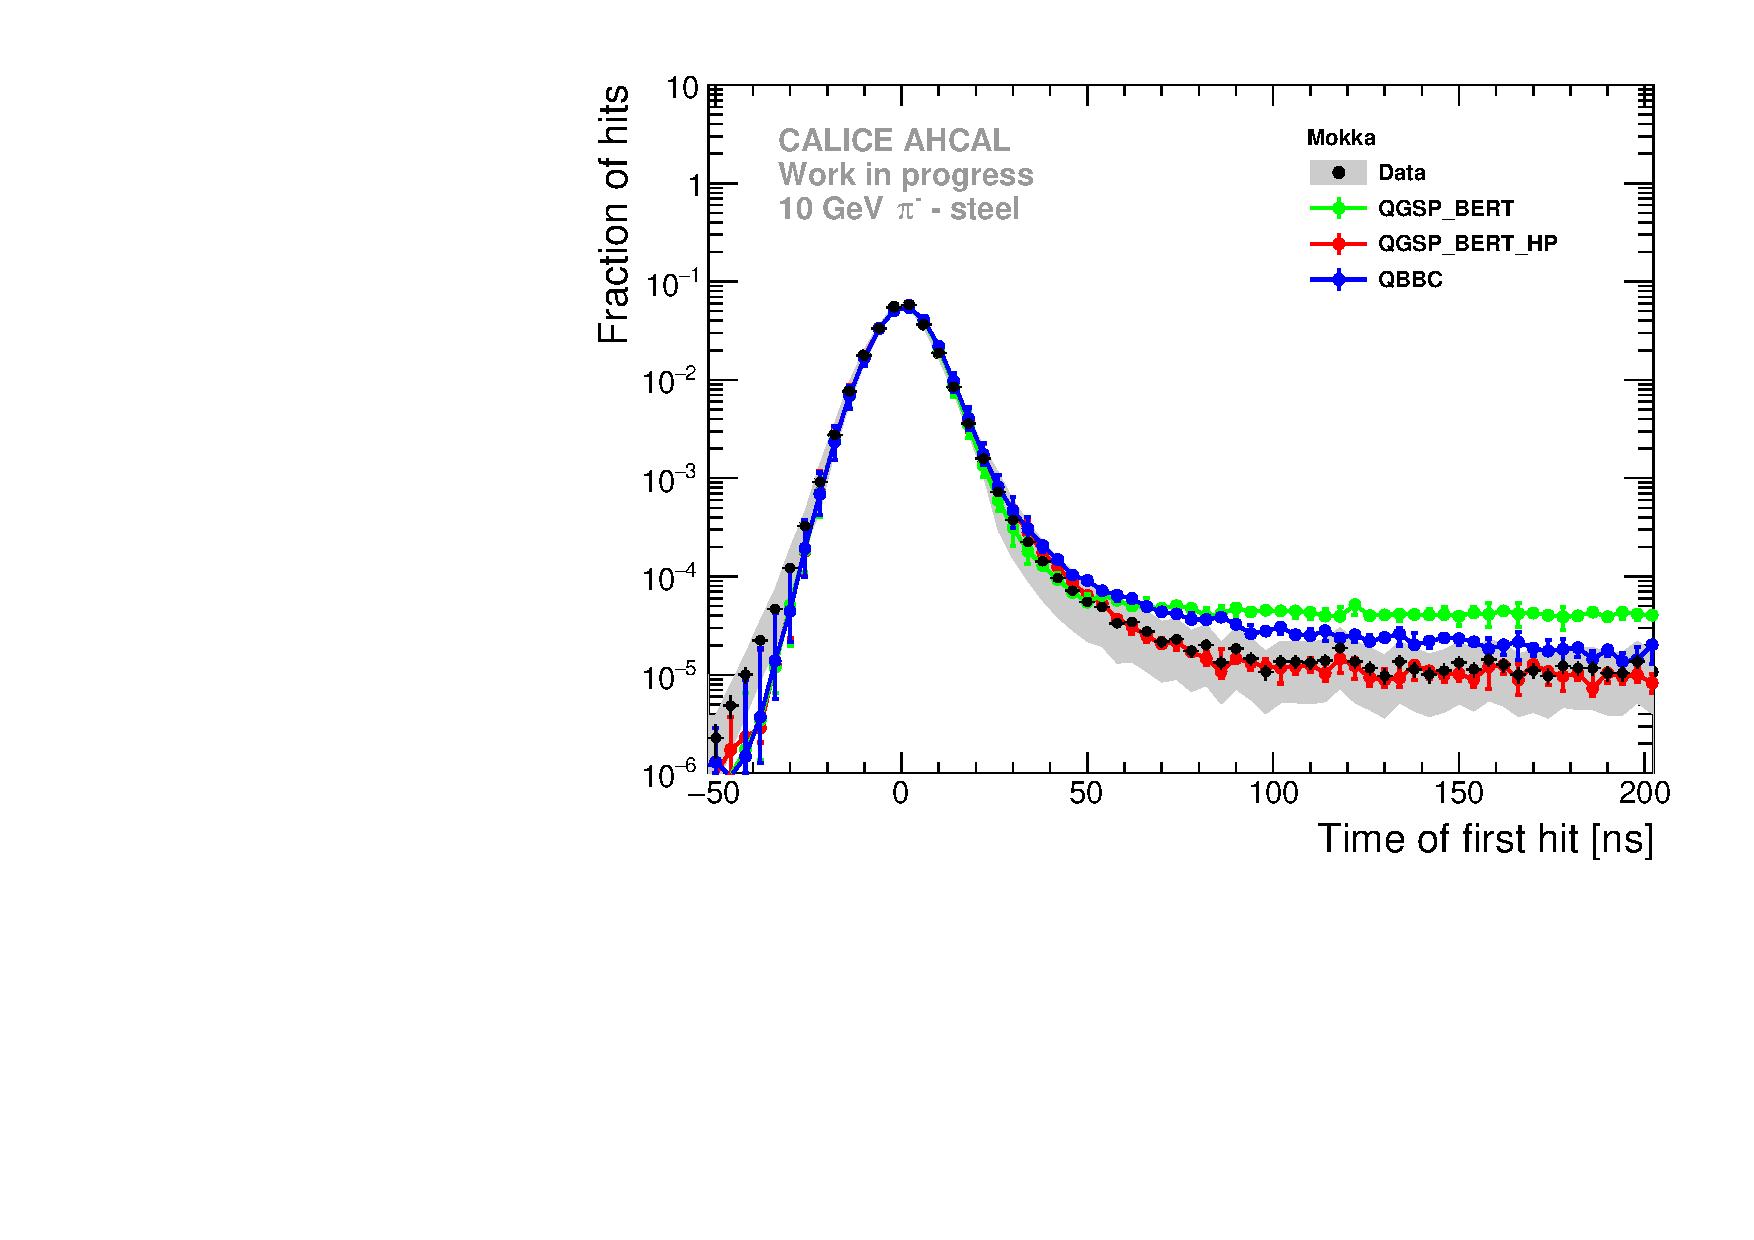
\includegraphics[width=1\textwidth]{../Thesis_Plots/Timing/Pions/Plots/Comparison_SimData_Pion10GeV_LateClusters.pdf}
		\caption{10 GeV.} \label{fig:dNdt_SimData_10GeV}
	\end{subfigure}
	\hfill
	\begin{subfigure}[t]{0.5\textwidth}
		\centering
		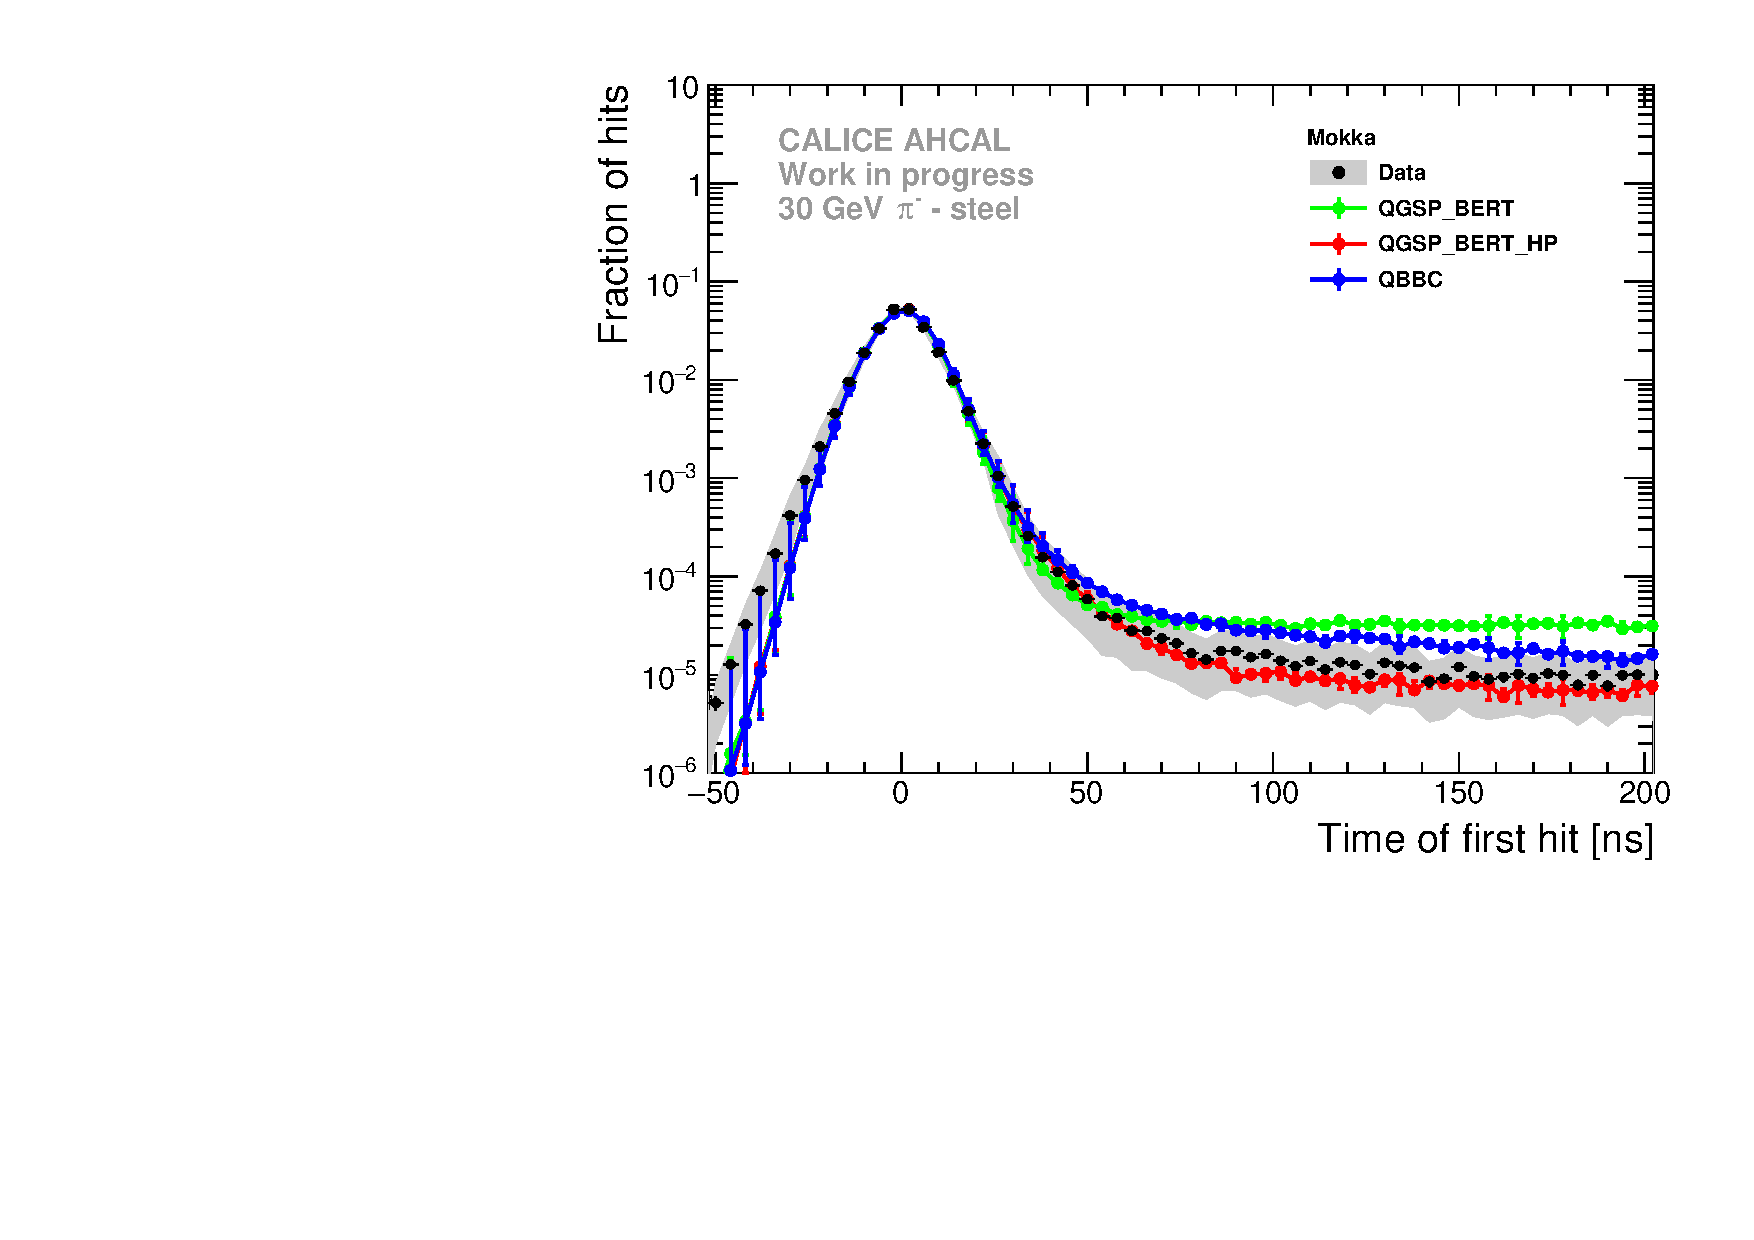
\includegraphics[width=1\textwidth]{../Thesis_Plots/Timing/Pions/Plots/Comparison_SimData_Pion30GeV_LateClusters.pdf}
		\caption{30 GeV.}\label{fig:dNdt_SimData_30GeV}
	\end{subfigure}
	\begin{subfigure}[t]{0.5\textwidth}
		\centering
		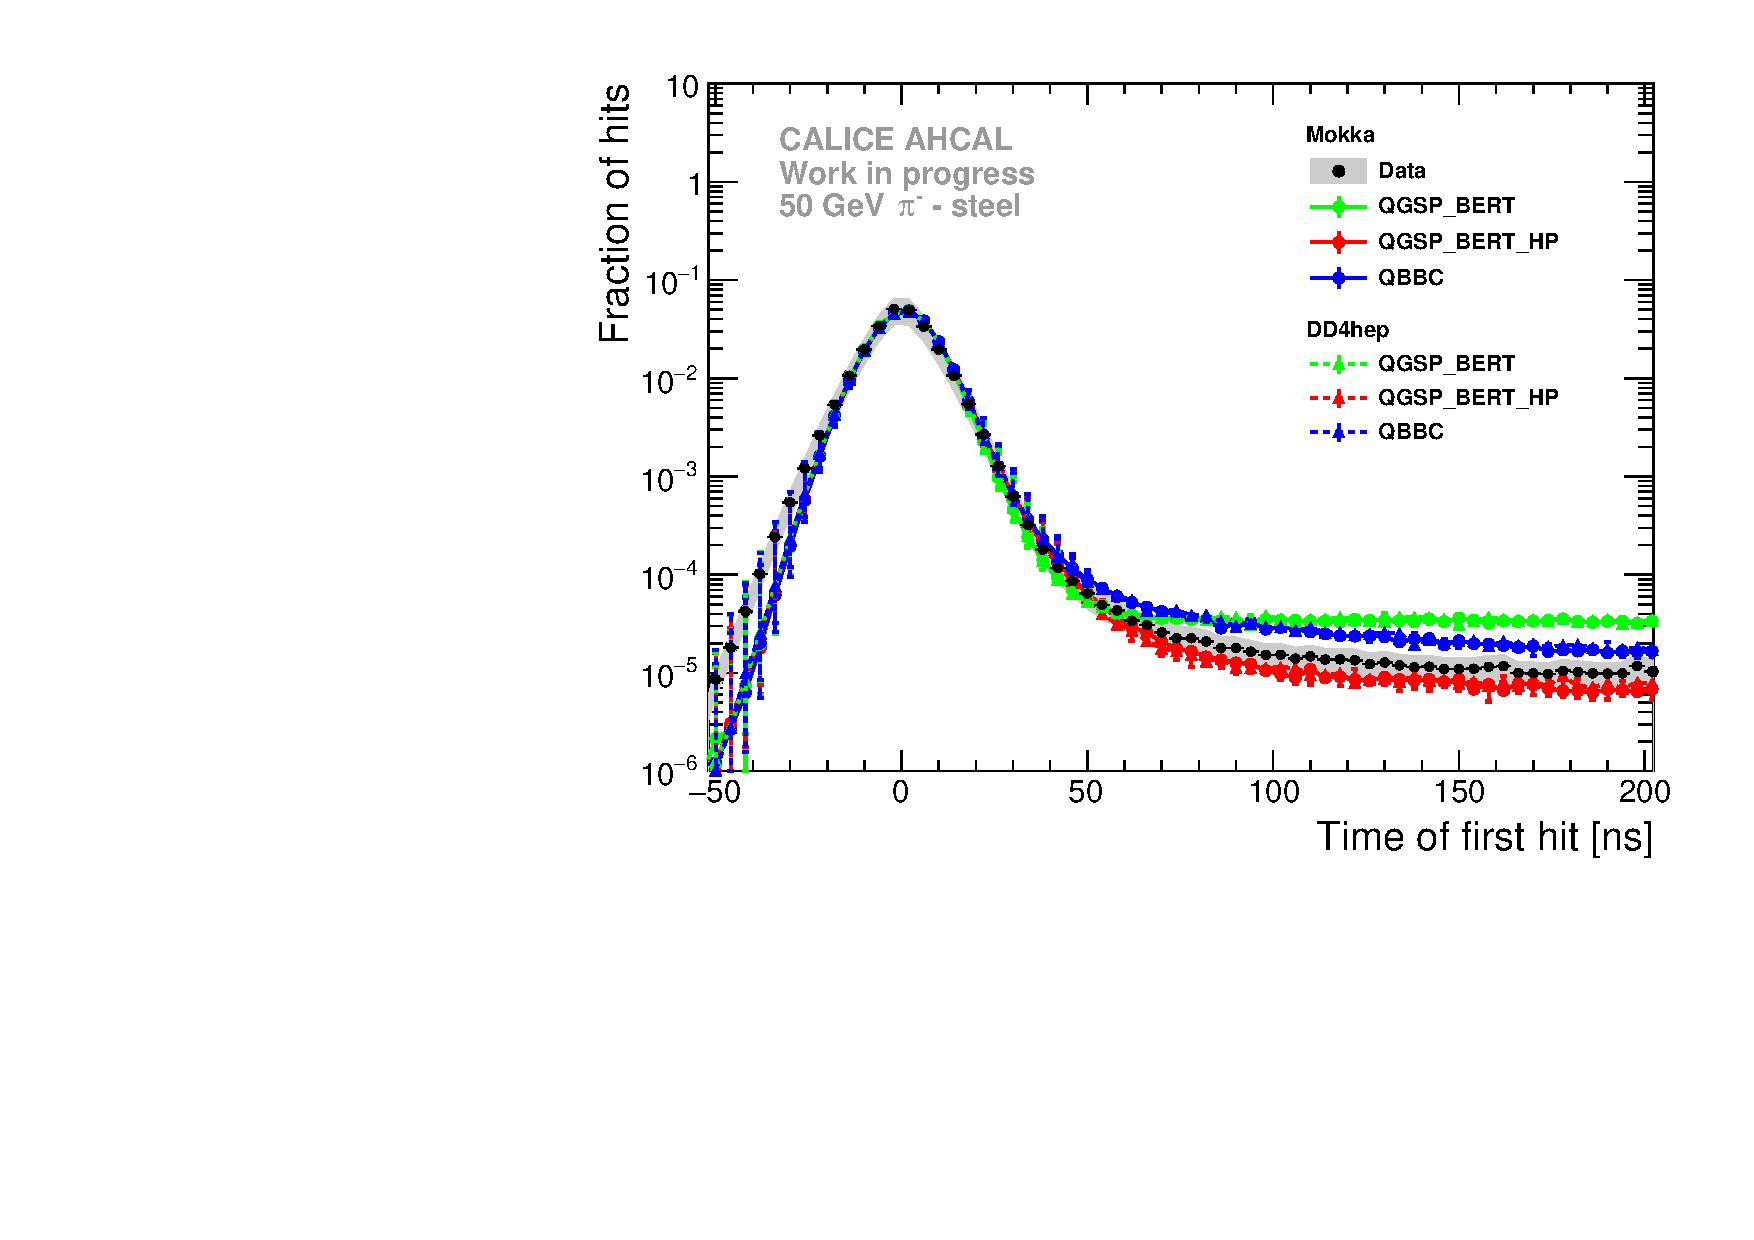
\includegraphics[width=1\textwidth]{../Thesis_Plots/Timing/Pions/Plots/Comparison_SimData_Pion50GeV_LateClusters.pdf}
		\caption{50 GeV.} \label{fig:dNdt_SimData_50GeV}
	\end{subfigure}
	\hfill
	\begin{subfigure}[t]{0.5\textwidth}
		\centering
		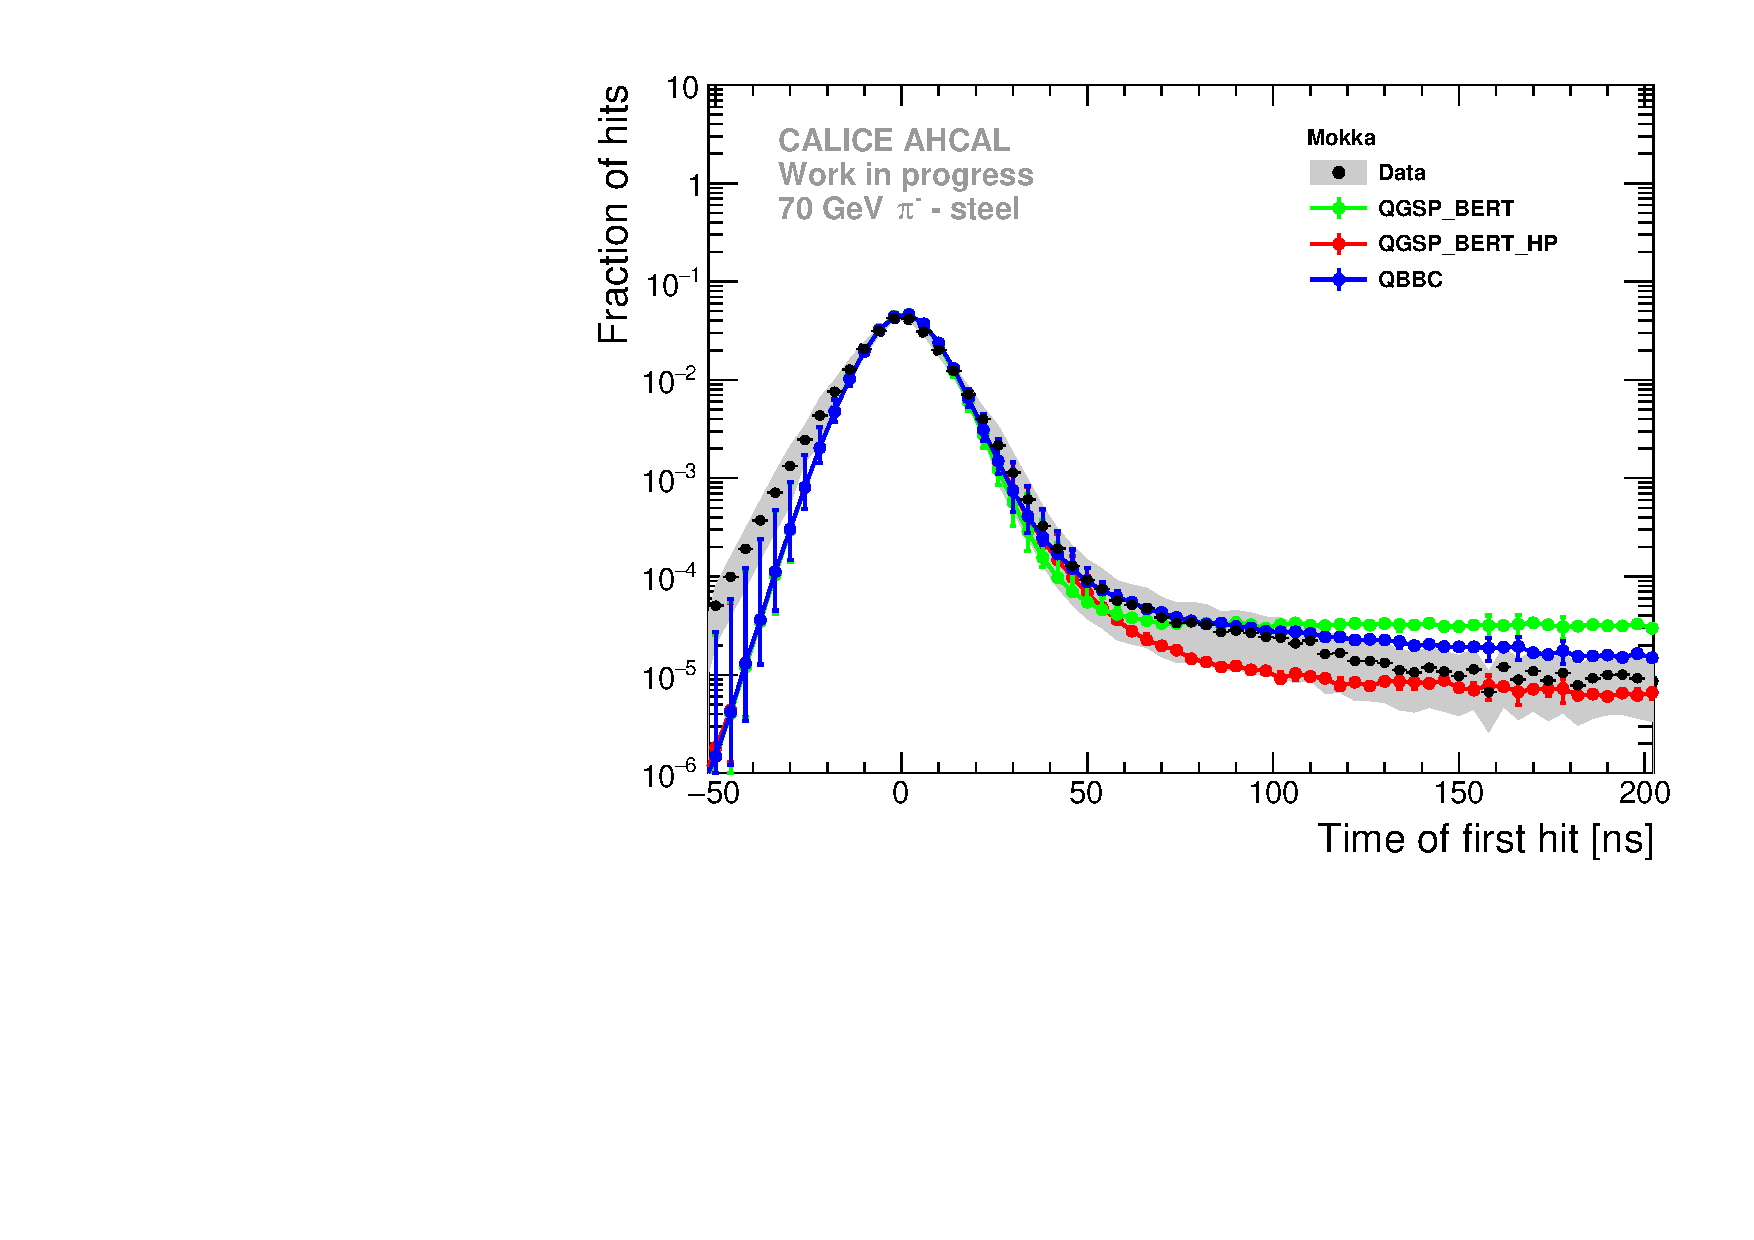
\includegraphics[width=1\textwidth]{../Thesis_Plots/Timing/Pions/Plots/Comparison_SimData_Pion70GeV_LateClusters.pdf}
		\caption{70 GeV.} \label{fig:dNdt_SimData_70GeV}
	\end{subfigure}
	\hfill
	\begin{subfigure}[t]{0.5\textwidth}
		\centering
		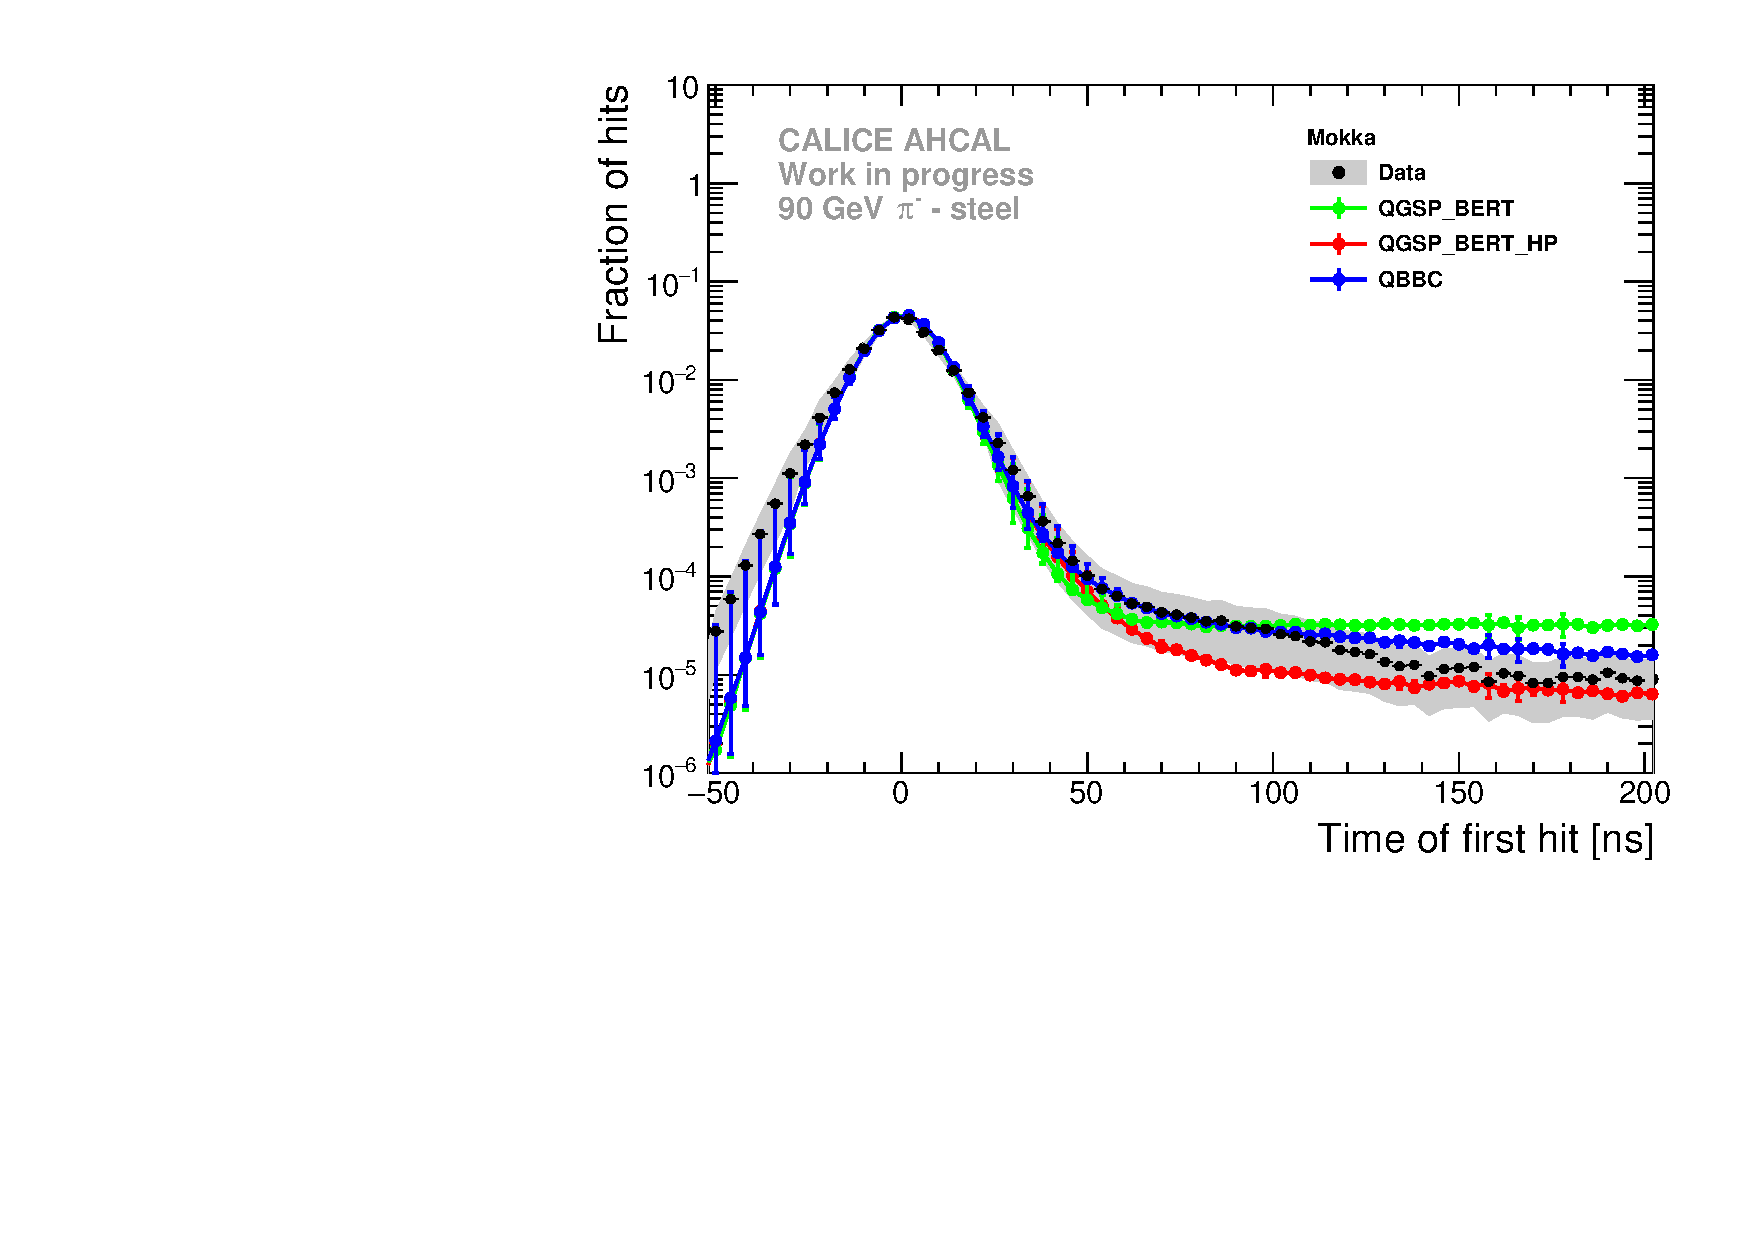
\includegraphics[width=1\textwidth]{../Thesis_Plots/Timing/Pions/Plots/Comparison_SimData_Pion90GeV_LateClusters.pdf}
		\caption{90 GeV.} \label{fig:dNdt_SimData_90GeV}
	\end{subfigure}
	\caption{Comparison between simulations and data of the time of first hit per bin time for pion beams between 10 GeV and 90 GeV. The grey and color bands shows the systematics.}
	\label{fig:dNdt_SimData_Comparison}
\end{figure}

The figure \ref{fig:Energy_SimData_Comparison} shows the mean time of first hit as a function of the hit energy. For 10 GeV pions, the simulation reproduces well the data within the systematics. For higher energies, a difference is visible in the region 0.5 to 1.5 MIP where the simulation is above the data. Above around 2 MIPs, the data and simulations agree well. QBBC and QGSP\_BERT seem higher in general over the full energy range showing that without precision neutron tracking, late depositions may be produced in large quantities within the systematics of the data, but the models can't be distinguished.
Moreover, the simulations seem to show an increase of the mean time of first hit at small hit energies with higher beam energy. The data does not reflect this.

\begin{figure}[htbp!]
	\begin{subfigure}[t]{0.5\textwidth}
		\centering
		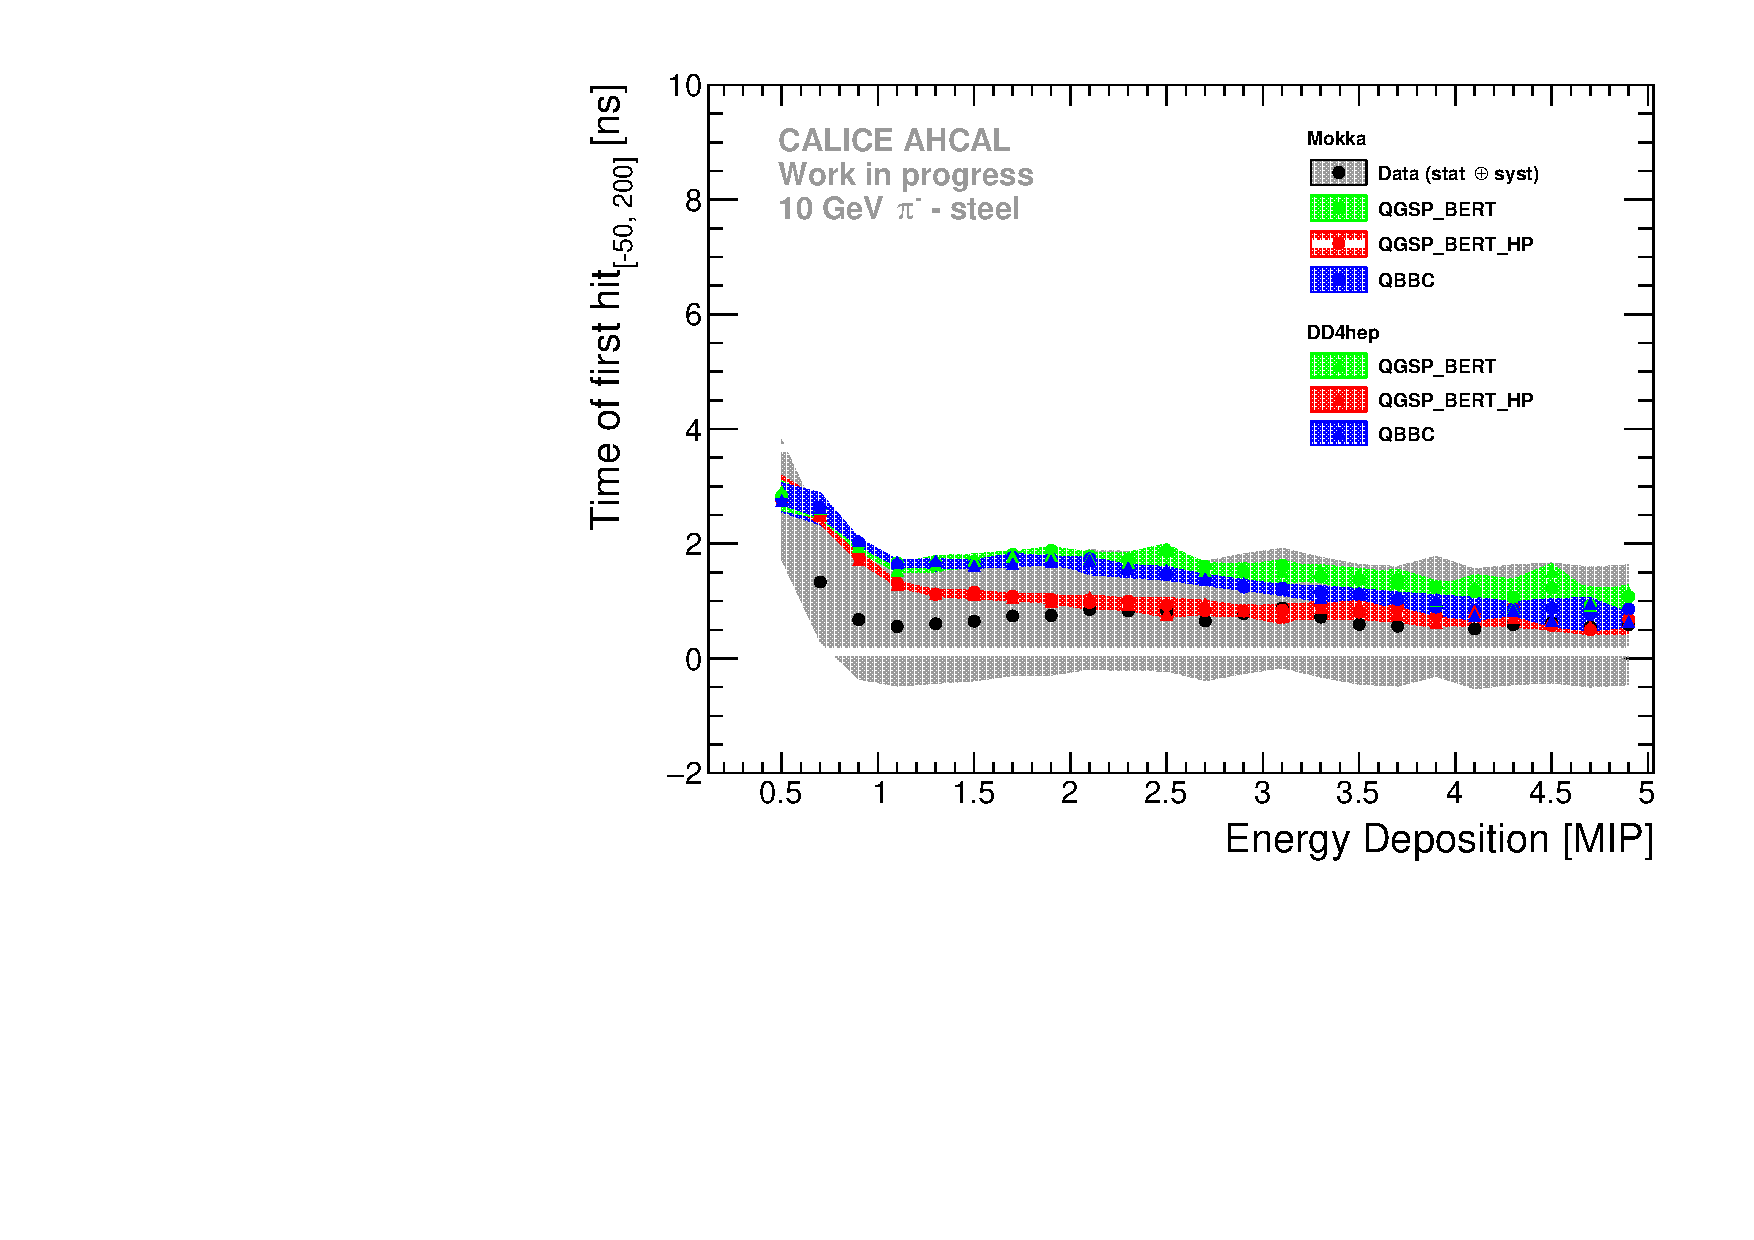
\includegraphics[width=1\textwidth]{../Thesis_Plots/Timing/Pions/Plots/ComparisonToSim/Time_Energy_10GeV.pdf}
		\caption{10 GeV.} \label{fig:Energy_SimData_10GeV}
	\end{subfigure}
	\hfill
	\begin{subfigure}[t]{0.5\textwidth}
		\centering
		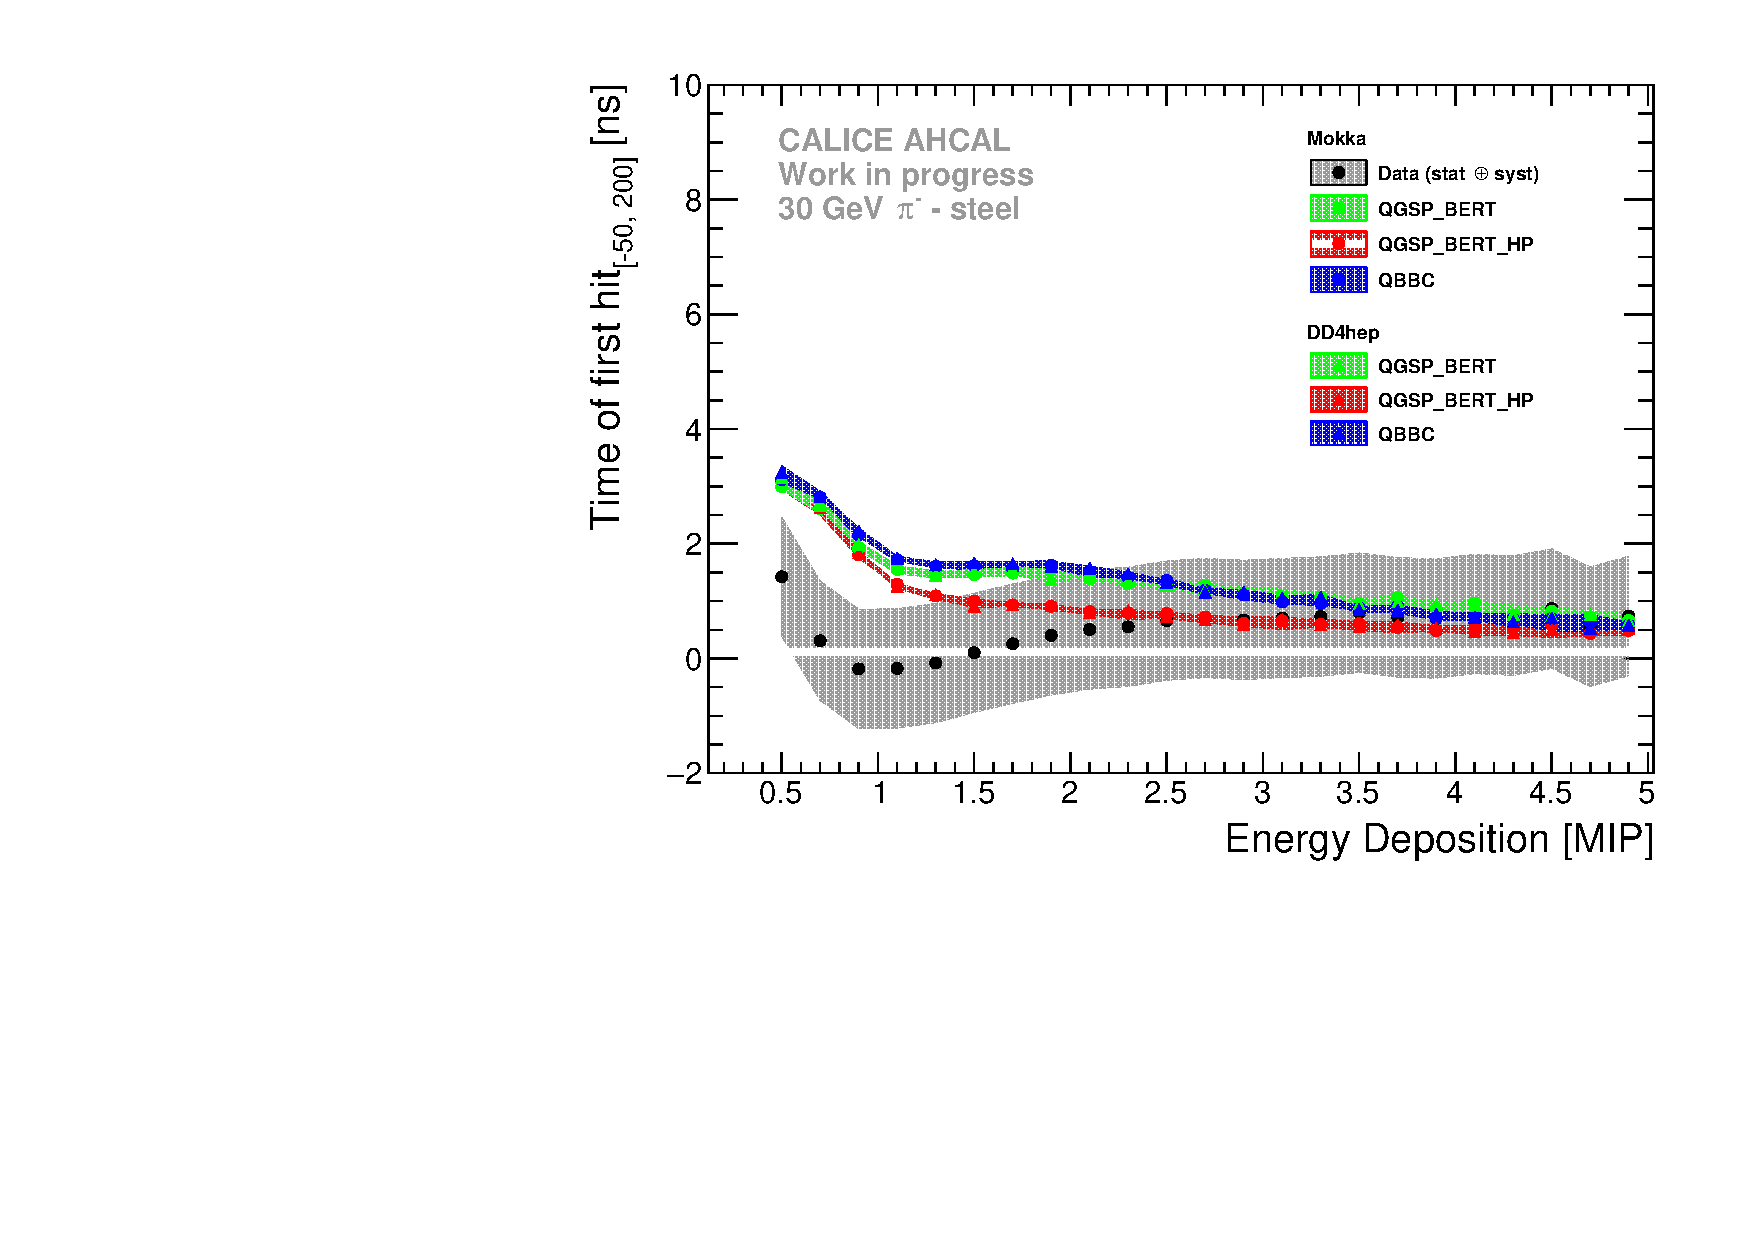
\includegraphics[width=1\textwidth]{../Thesis_Plots/Timing/Pions/Plots/ComparisonToSim/Time_Energy_30GeV.pdf}
		\caption{30 GeV.}\label{fig:Energy_SimData_30GeV}
	\end{subfigure}
	\begin{subfigure}[t]{0.5\textwidth}
		\centering
		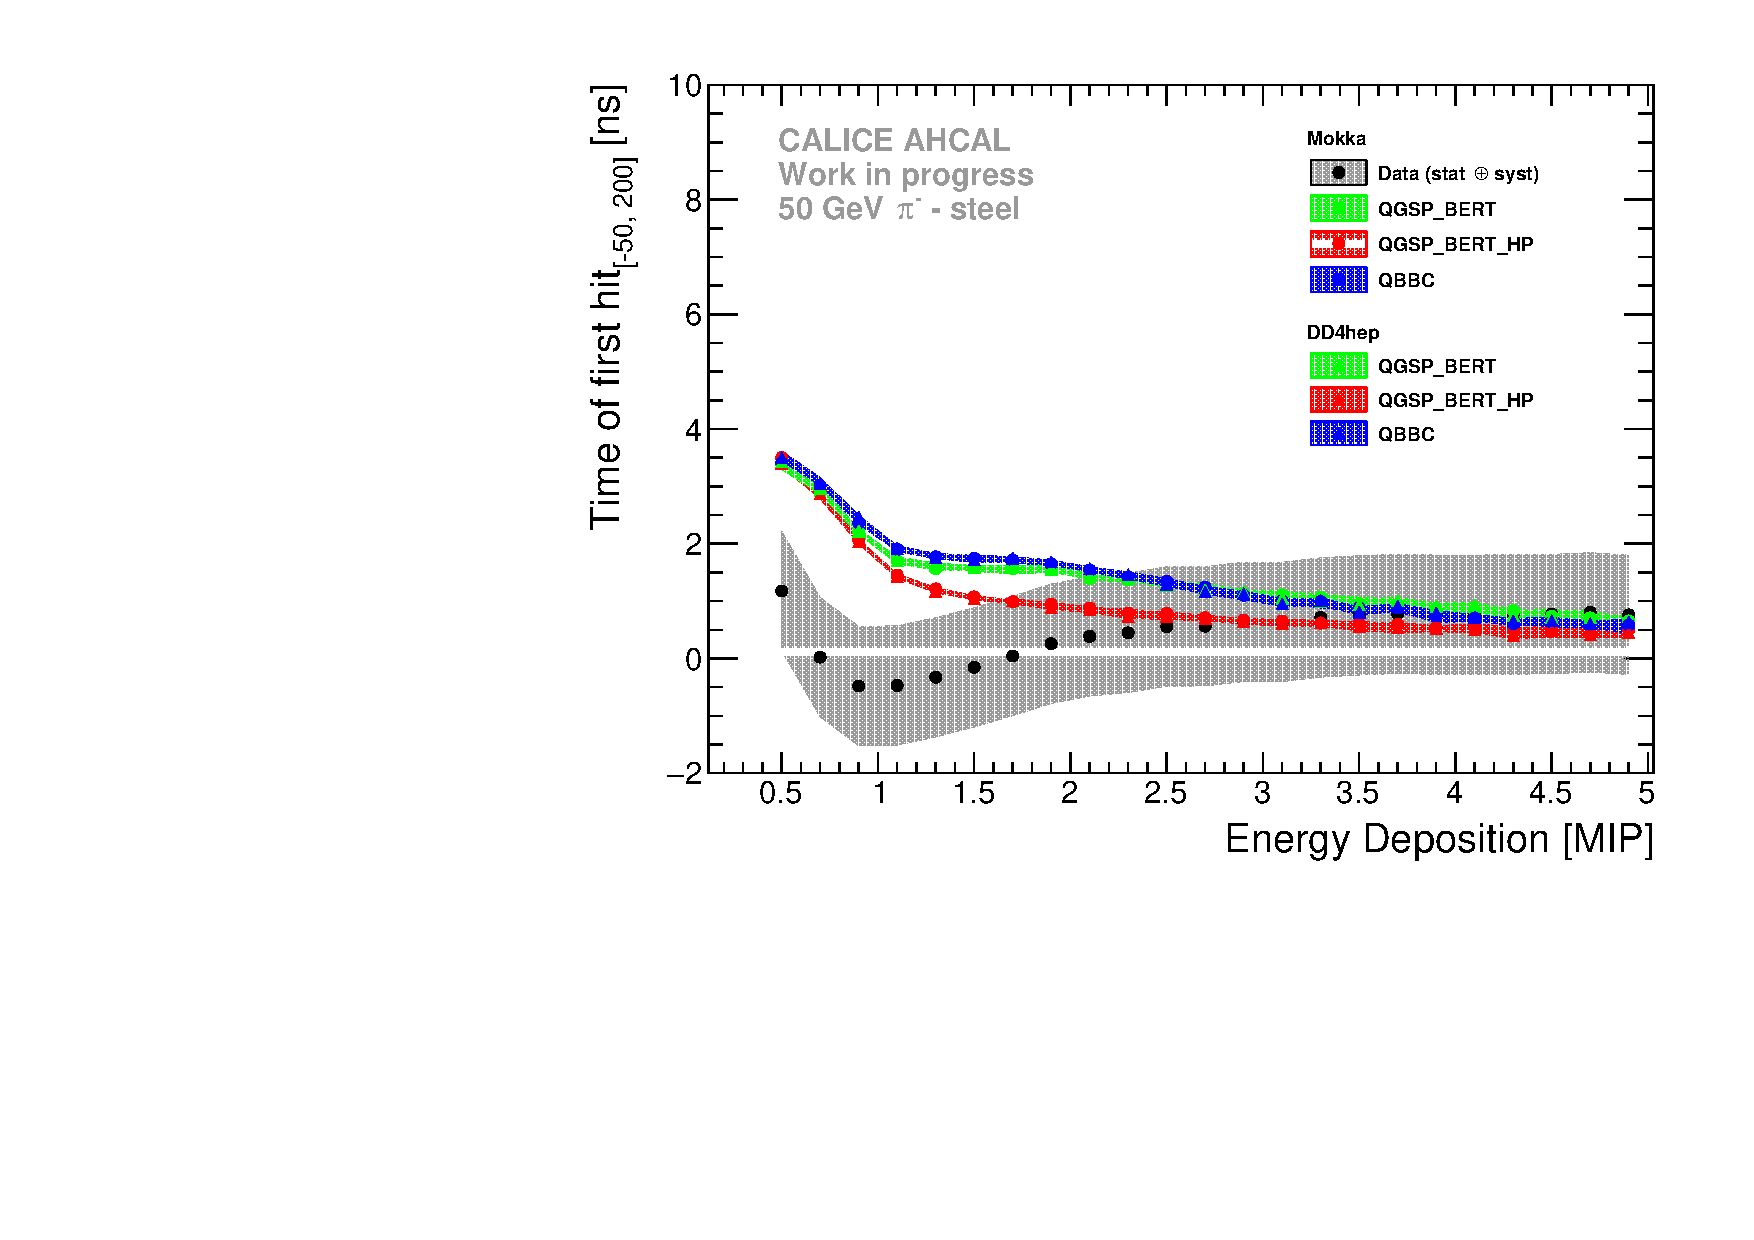
\includegraphics[width=1\textwidth]{../Thesis_Plots/Timing/Pions/Plots/ComparisonToSim/Time_Energy_50GeV.pdf}
		\caption{50 GeV.} \label{fig:Energy_SimData_50GeV}
	\end{subfigure}
	\hfill
	\begin{subfigure}[t]{0.5\textwidth}
		\centering
		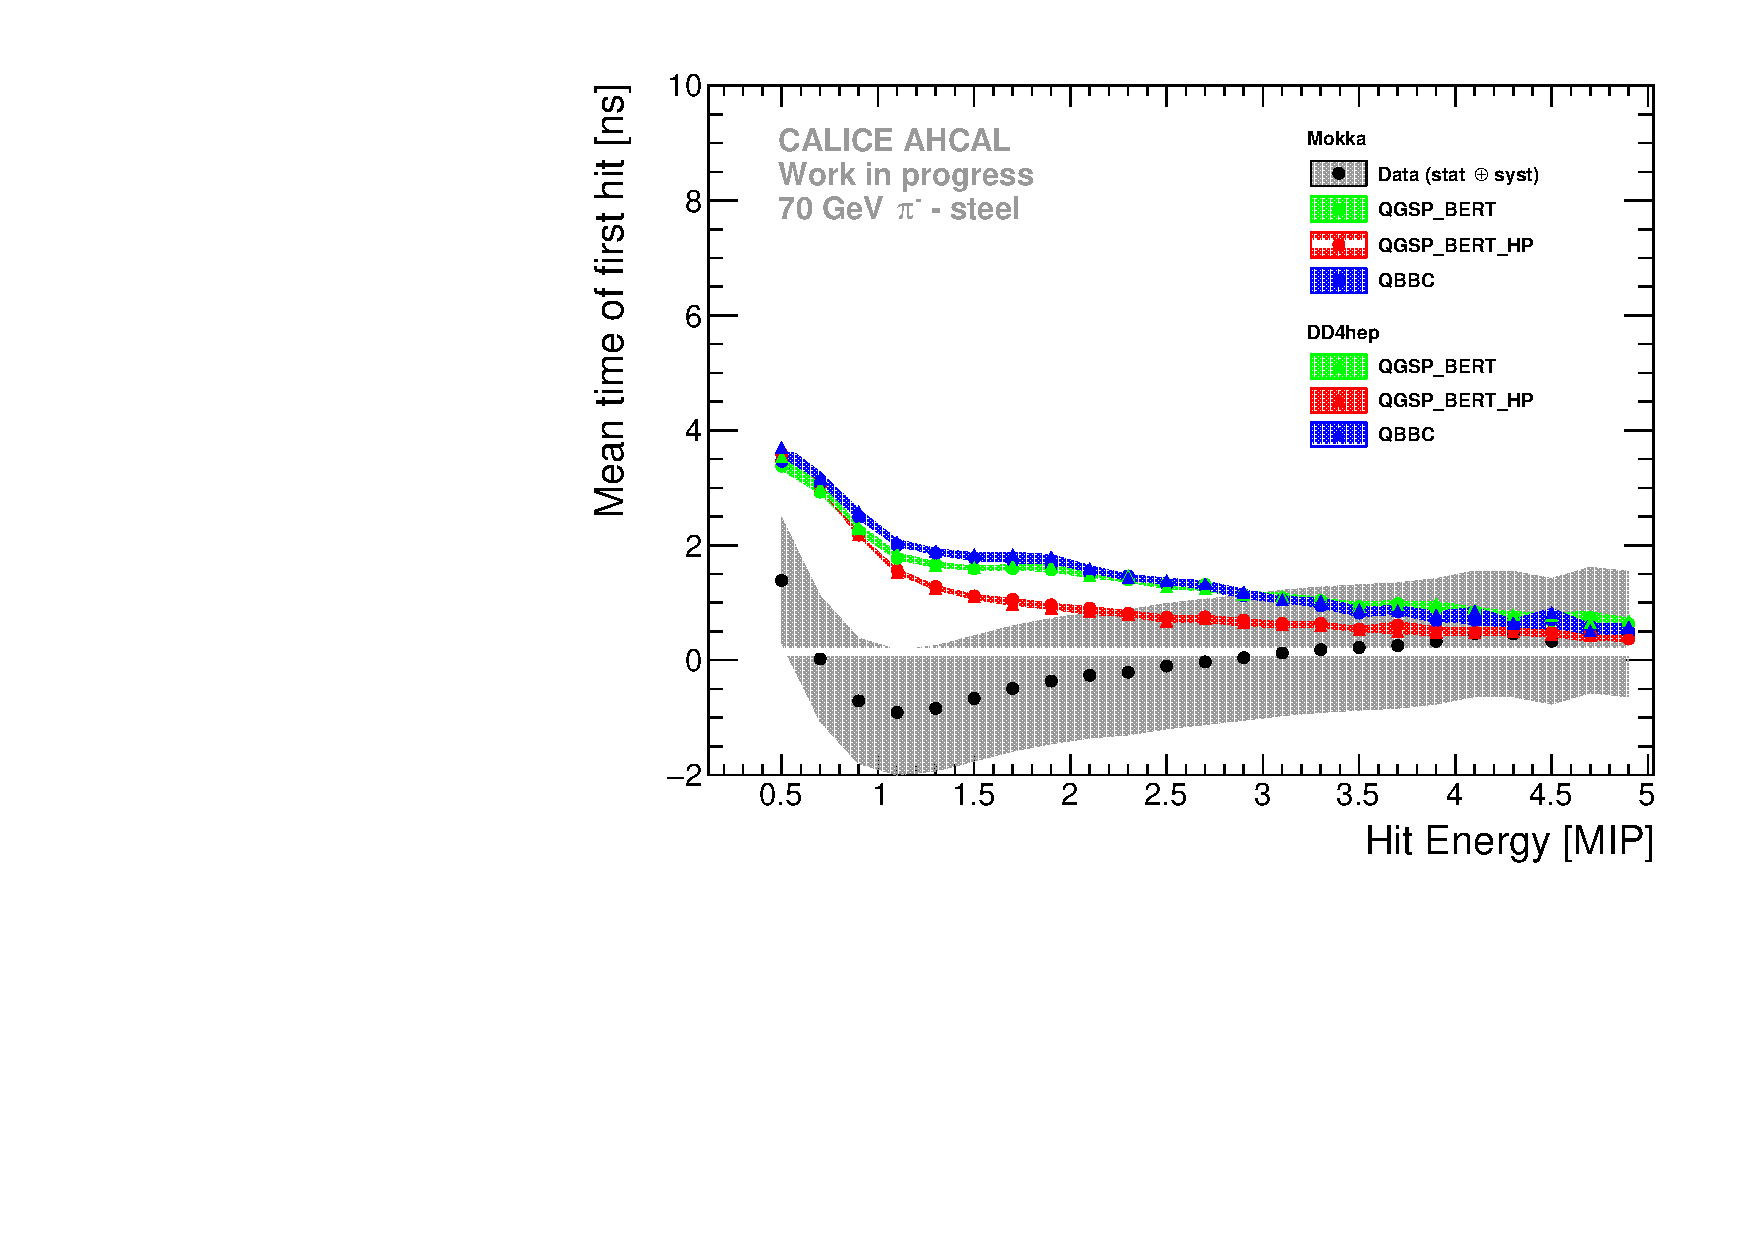
\includegraphics[width=1\textwidth]{../Thesis_Plots/Timing/Pions/Plots/ComparisonToSim/Time_Energy_70GeV.pdf}
		\caption{70 GeV.} \label{fig:Energy_SimData_70GeV}
	\end{subfigure}
	\hfill
	\begin{subfigure}[t]{0.5\textwidth}
		\centering
		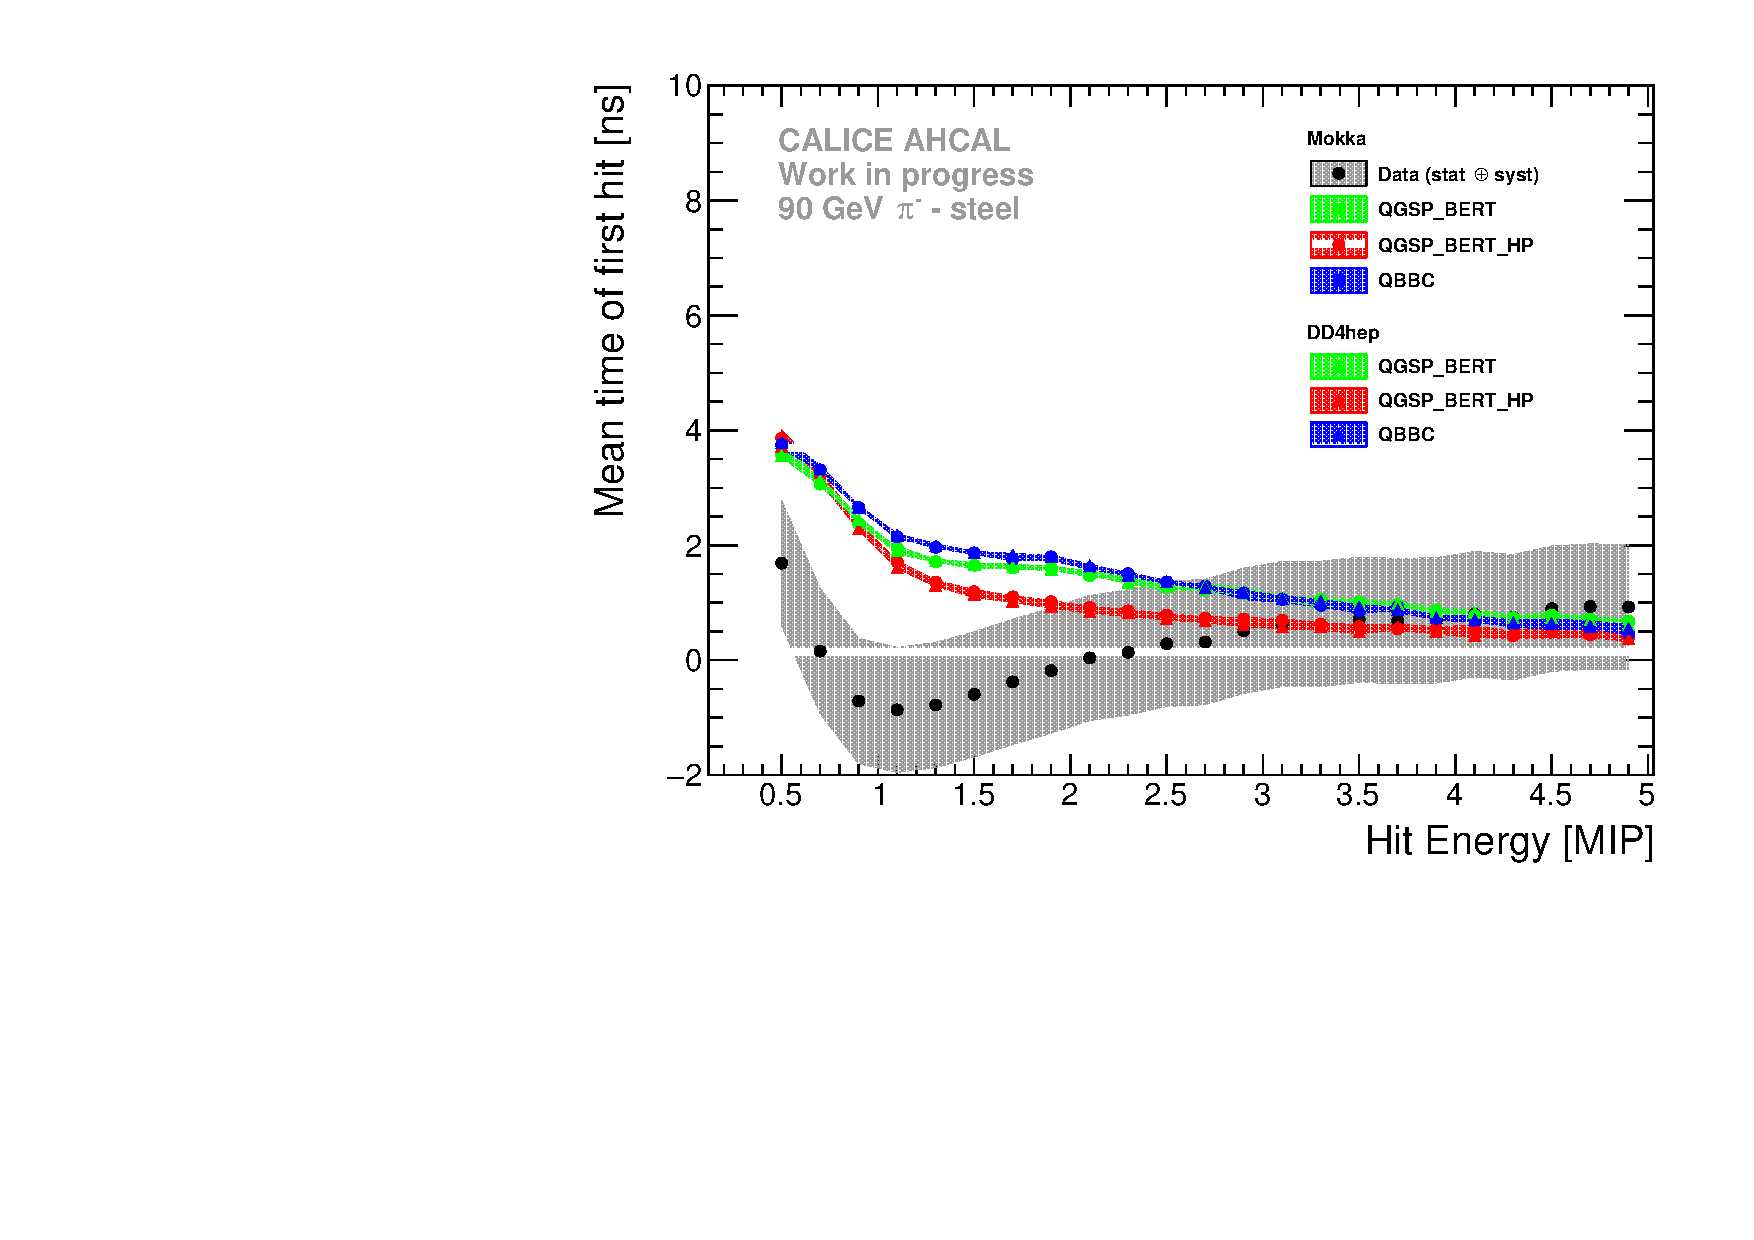
\includegraphics[width=1\textwidth]{../Thesis_Plots/Timing/Pions/Plots/ComparisonToSim/Time_Energy_90GeV.pdf}
		\caption{90 GeV.} \label{fig:Energy_SimData_90GeV}
	\end{subfigure}
	\caption{Comparison between simulations and data of the time of first hit as function of the hit energy for pion beams between 10 GeV and 90 GeV. The grey and color bands shows the systematics.}
	\label{fig:Energy_SimData_Comparison}
\end{figure}

\section{Radial dependence of timing profiles}

As shown in the previous section, the prompt part of the shower is dominated by EM sub-showers and relativistic particles. The delayed part is coming from mostly evaporation and spallation low energy neutrons. It is expected that the former is concentrated near the shower axis, while the latter, is spread out laterally as these neutrons can travel far away in the calorimeter before interacting. This is investigated by looking at the mean time of first hit as a function of the distance to the shower center of gravity defined in the [x,y] plane with the exception of the muon data, where the position in the detector relative to (0,0) is used. This is shown in figures \ref{fig:Radius_Comparison_SSF} and \ref{fig:Radius_Comparison_BL} for the layers from 3 to 10 and the layers from 11 to 14 separately.

\begin{figure}[htbp!]
	\begin{subfigure}[t]{0.5\textwidth}
		\centering
		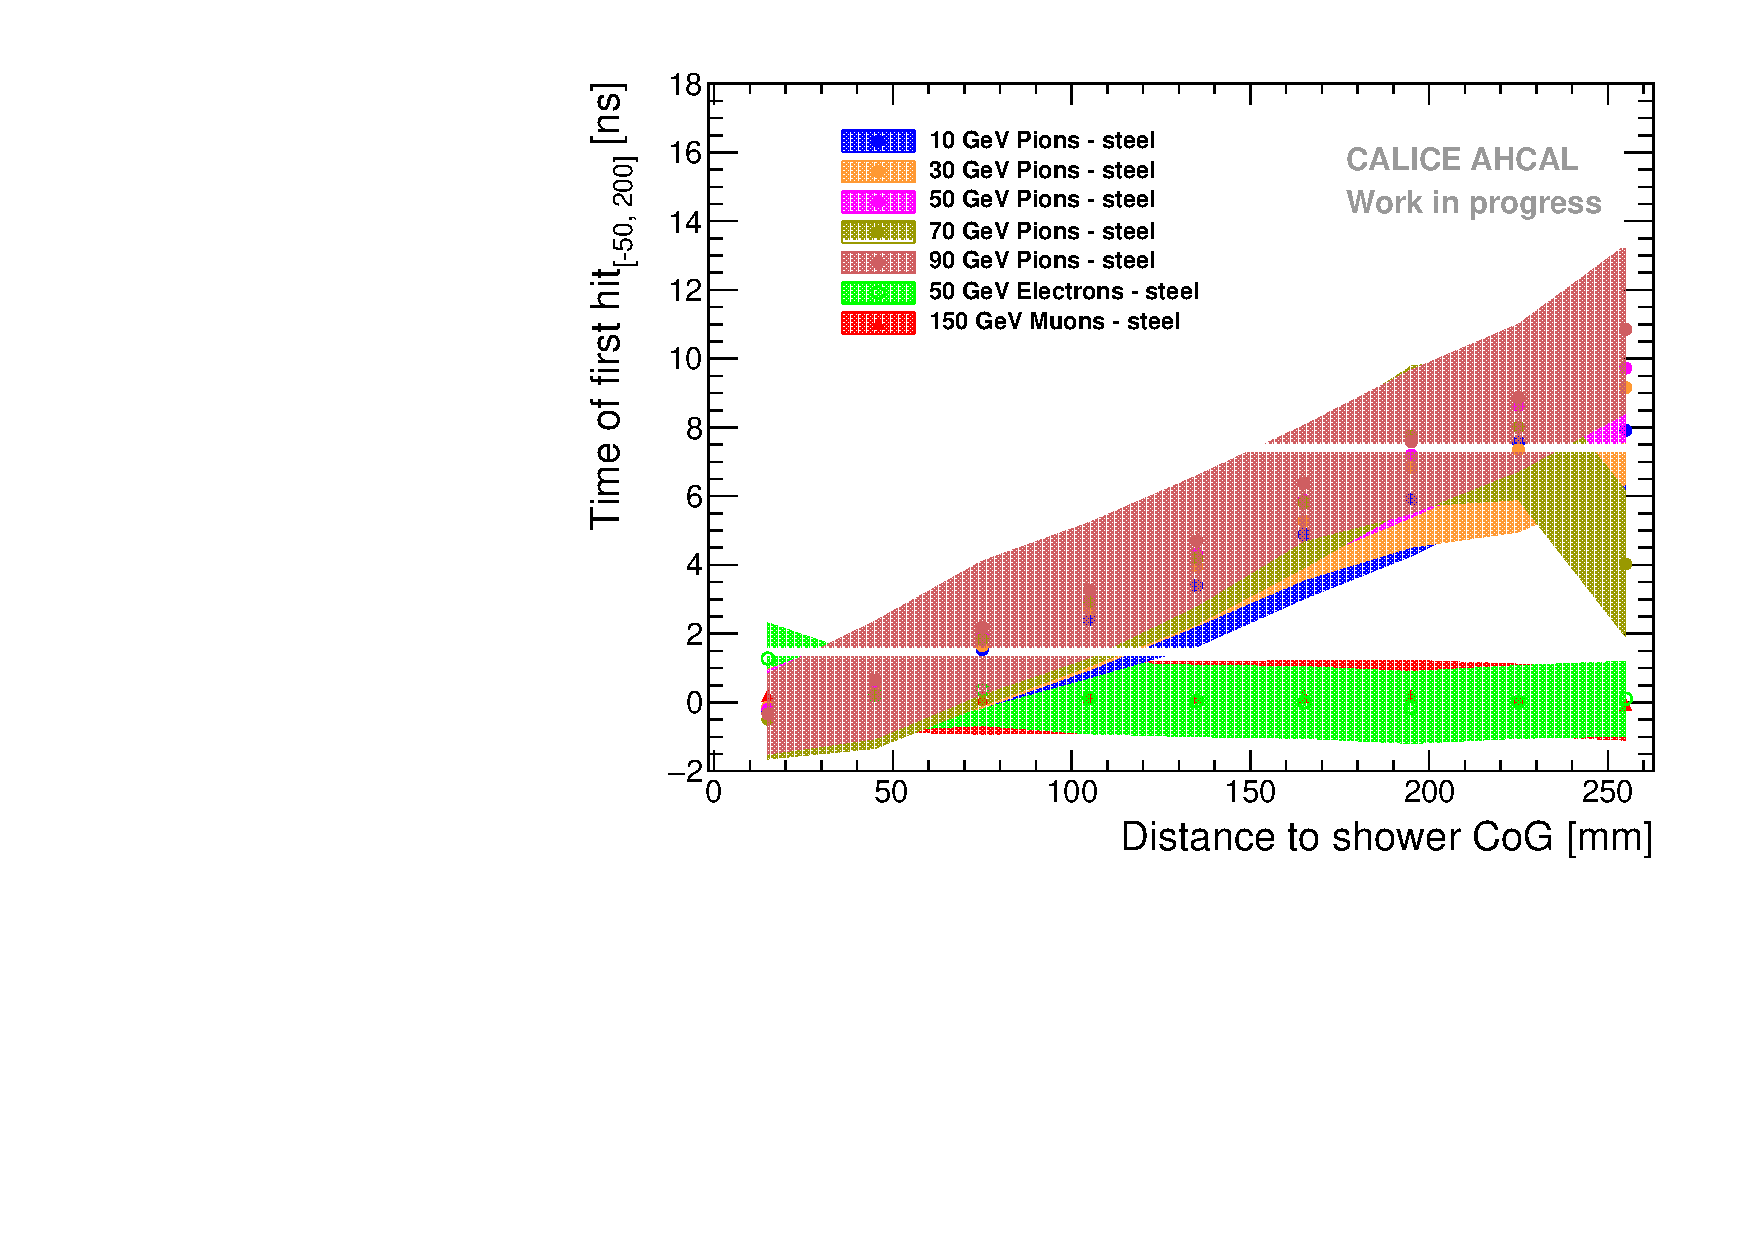
\includegraphics[width=1\textwidth]{../Thesis_Plots/Timing/Pions/Plots/Timing_Radius_Comparison_ShortAsymRange_SSF.pdf}
		\caption{Small layers from 3 to 10.}\label{fig:Radius_Comparison_SSF}
	\end{subfigure}
	\hfill
	\begin{subfigure}[t]{0.5\textwidth}
		\centering
		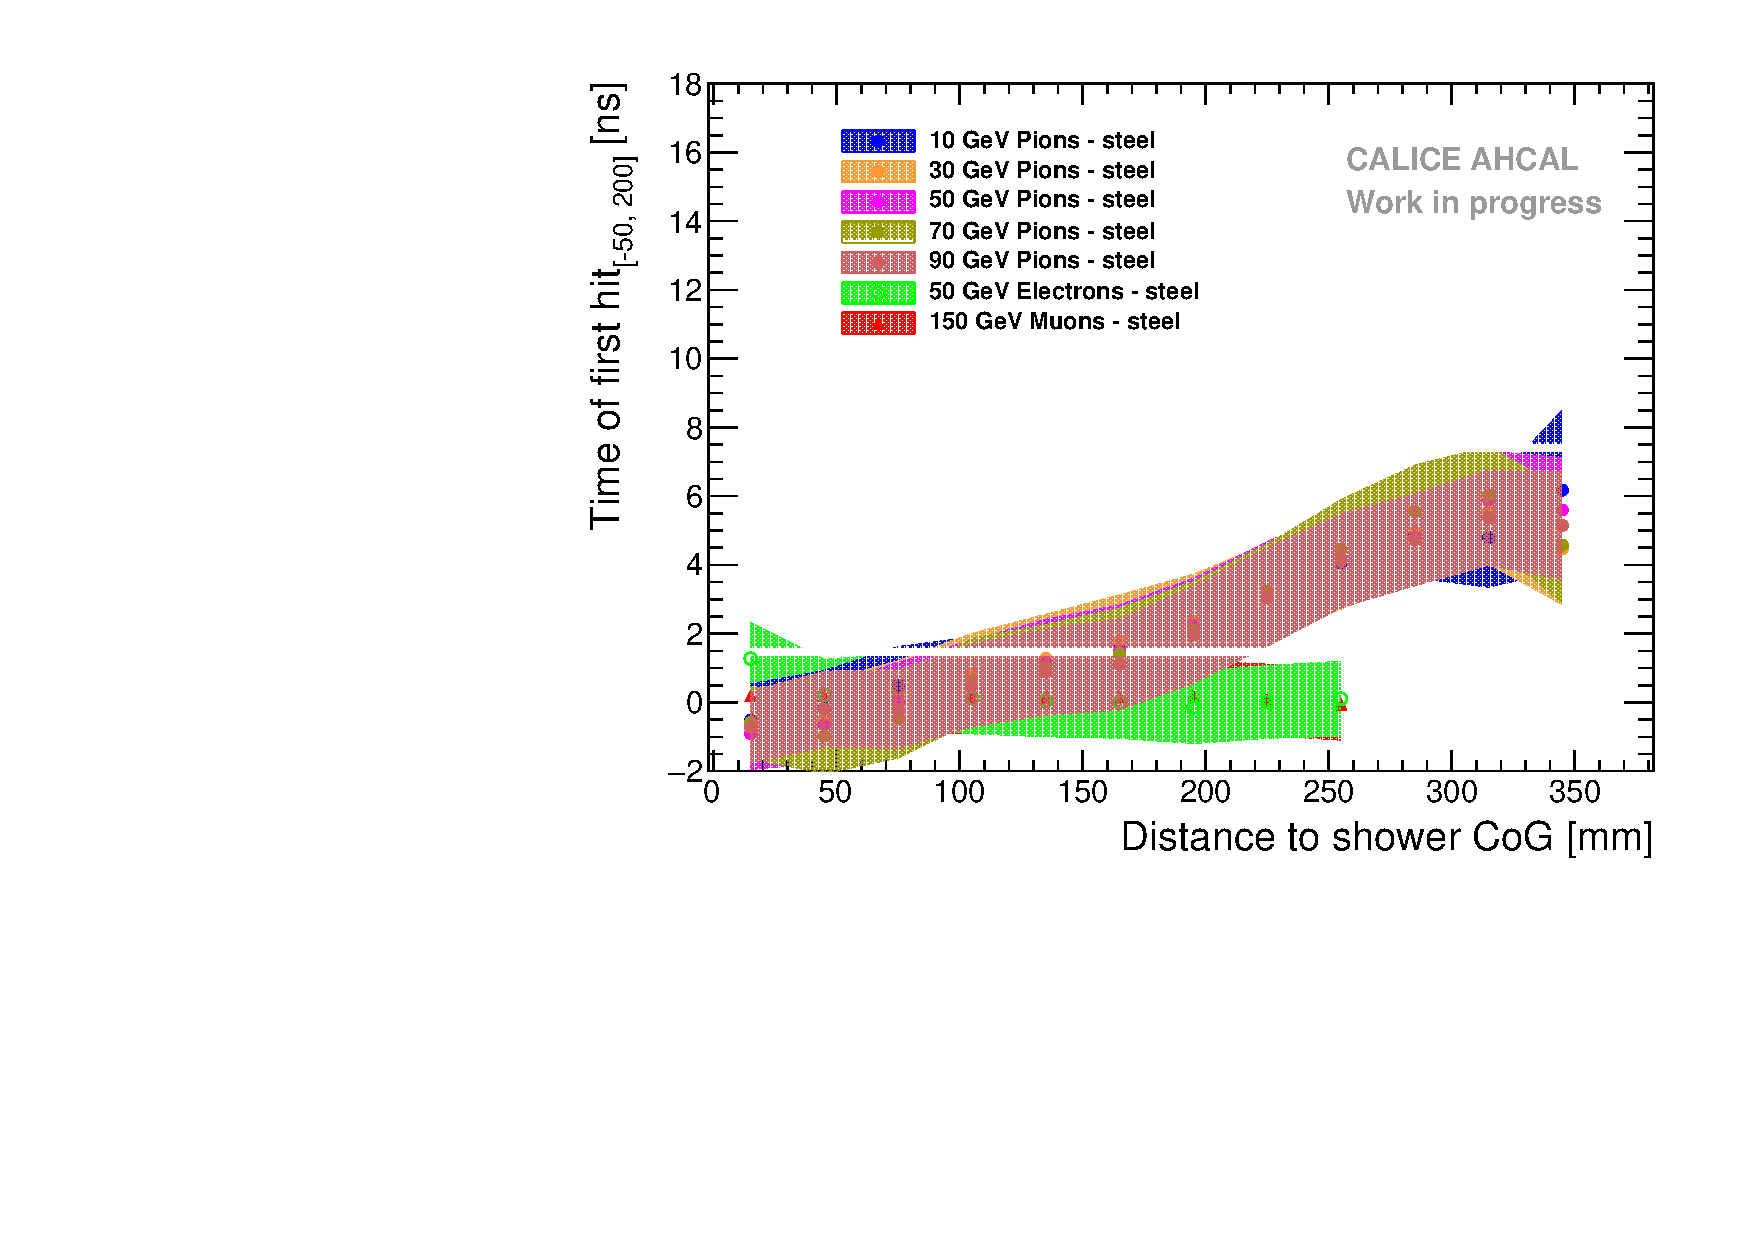
\includegraphics[width=1\textwidth]{../Thesis_Plots/Timing/Pions/Plots/Timing_Radius_Comparison_ShortAsymRange_BL.pdf}
		\caption{Big layers from 11 to 14.}\label{fig:Radius_Comparison_BL}
	\end{subfigure}
	\caption{Radial shower timing profile of the time of first hit for muon, electron and pion beams. The left plot shows the timing profile for the small layers and the right profile shows the timing profile for big layers. The explanation for the separation is described in the text. The systematics are shown by the color bands.}
	\label{fig:RadialTiming}
\end{figure}

For muons and electrons, the mean time of the first hit does not vary with the increase of radius showing that the processes involved are prompt and independent of the position. On the contrary for hadronic showers, it shows an increase with the distance to the shower axis for both type of boards, though the slopes are different with the small layers presenting a steeper slope. This is consistent with the expectation of the core of the shower depositing promptly most of the energy via EM sub-showers and relativistic particles near the shower axis. This is followed by a hadronic halo which contributes to delayed signals by mainly neutron-induced processes. For the small layers, the time of first hit varies between 0 ns at small radius and 10 ns at 25 cm. For the big layers, it varies between 0 ns near the shower axis, 4 ns at 25 cm and 6 ns at 35 cm. This shows a relative difference between both distributions. This is thought to come from the fact that different parts of the shower are sampled in the front/back of the calorimeter respectively depending on the position of the start of the shower.

To confirm this, I investigated the time of first hit as function of the radius to the shower axis at a constant distance between the layer investigated and the first hard interaction (\acrshort{fhi}) layer of the hadronic shower. First, a small algorithm for a shower start finder to find the layer of the first hard interaction had to be written. This is based on previous work \cite{CaN026} with slight modifications due to the fact that some of the layers in the front of the detector show a bad performance with many non-working channels.

The basics of the algorithm was to find the primary track and determine the shower start layer. To determine the shower start layer $s_{layer}$, the number of hits $n_{Hits}^{i, i+1}$ between the layer $i$ and $i+1$ is counted. If $n_{Hits}^{i, i+1} > 6$, the shower is considered started between layer $i$ and $i+1$. To determine the correct layer, the energy sum between layer $i$, $i+1$, $i+2$ and $i+3$ is checked such as:
\begin{equation*}
	s_{layer} =
	\begin{cases}
		i, & \text{if} \: E_{sum}^{i+2} < E_{sum}^{i} \:\&\: (E_{sum}^{i+3} < E_{sum}^{i}) \:\&\: (E_{sum}^{i+3} + E_{sum}^{i+2}) < (E_{sum}^{i+1} + E_{sum}^{i}) \\
		i-1, & \text{otherwise}
	\end{cases}
\end{equation*}

If an event was found in this case, a check on the length of the track was performed and it was required to be $>3$ hits on a track. A simple check on the performance of the algorithm was done by looking at the difference between the reconstructed layer of the FHI and the Monte-Carlo truth as well as the correlation between both. This is shown in figures \ref{fig:Diff_FHI_RecoMC} and \ref{fig:Corr_FHI_RecoMC}. The performance of the algorithm is good enough in order to get a good estimate of the FHI layer and has a small tendency to reconstruct the FHI at a deeper layer.

\begin{figure}[htbp!]
	\begin{subfigure}[t]{0.5\textwidth}
		\centering
		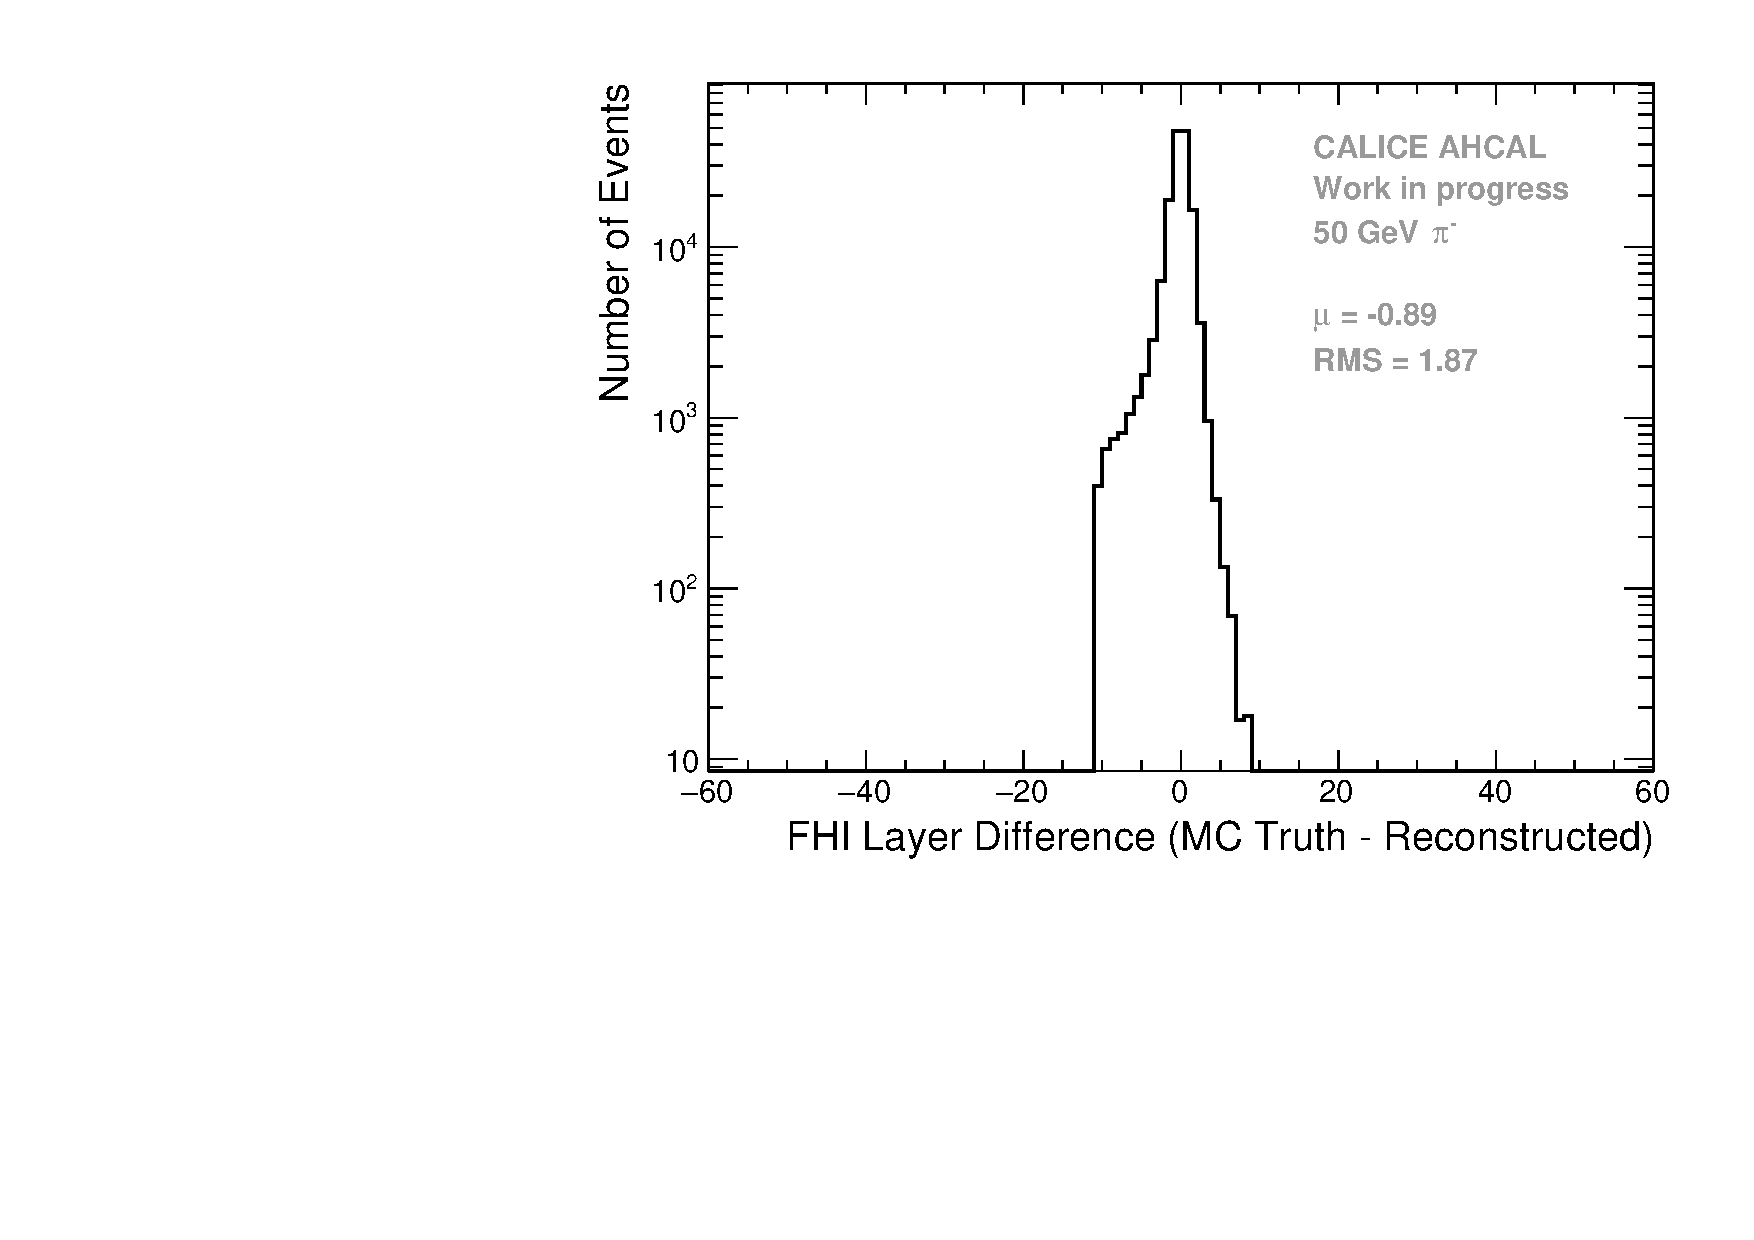
\includegraphics[width=1\textwidth]{../Thesis_Plots/Timing/Pions/Plots/ShowerStart_Difference_noOptimisation.pdf}
		\caption{Difference between reconstructed FHI and MC truth layer.}\label{fig:Diff_FHI_RecoMC}
	\end{subfigure}
	\hfill
	\begin{subfigure}[t]{0.5\textwidth}
		\centering
		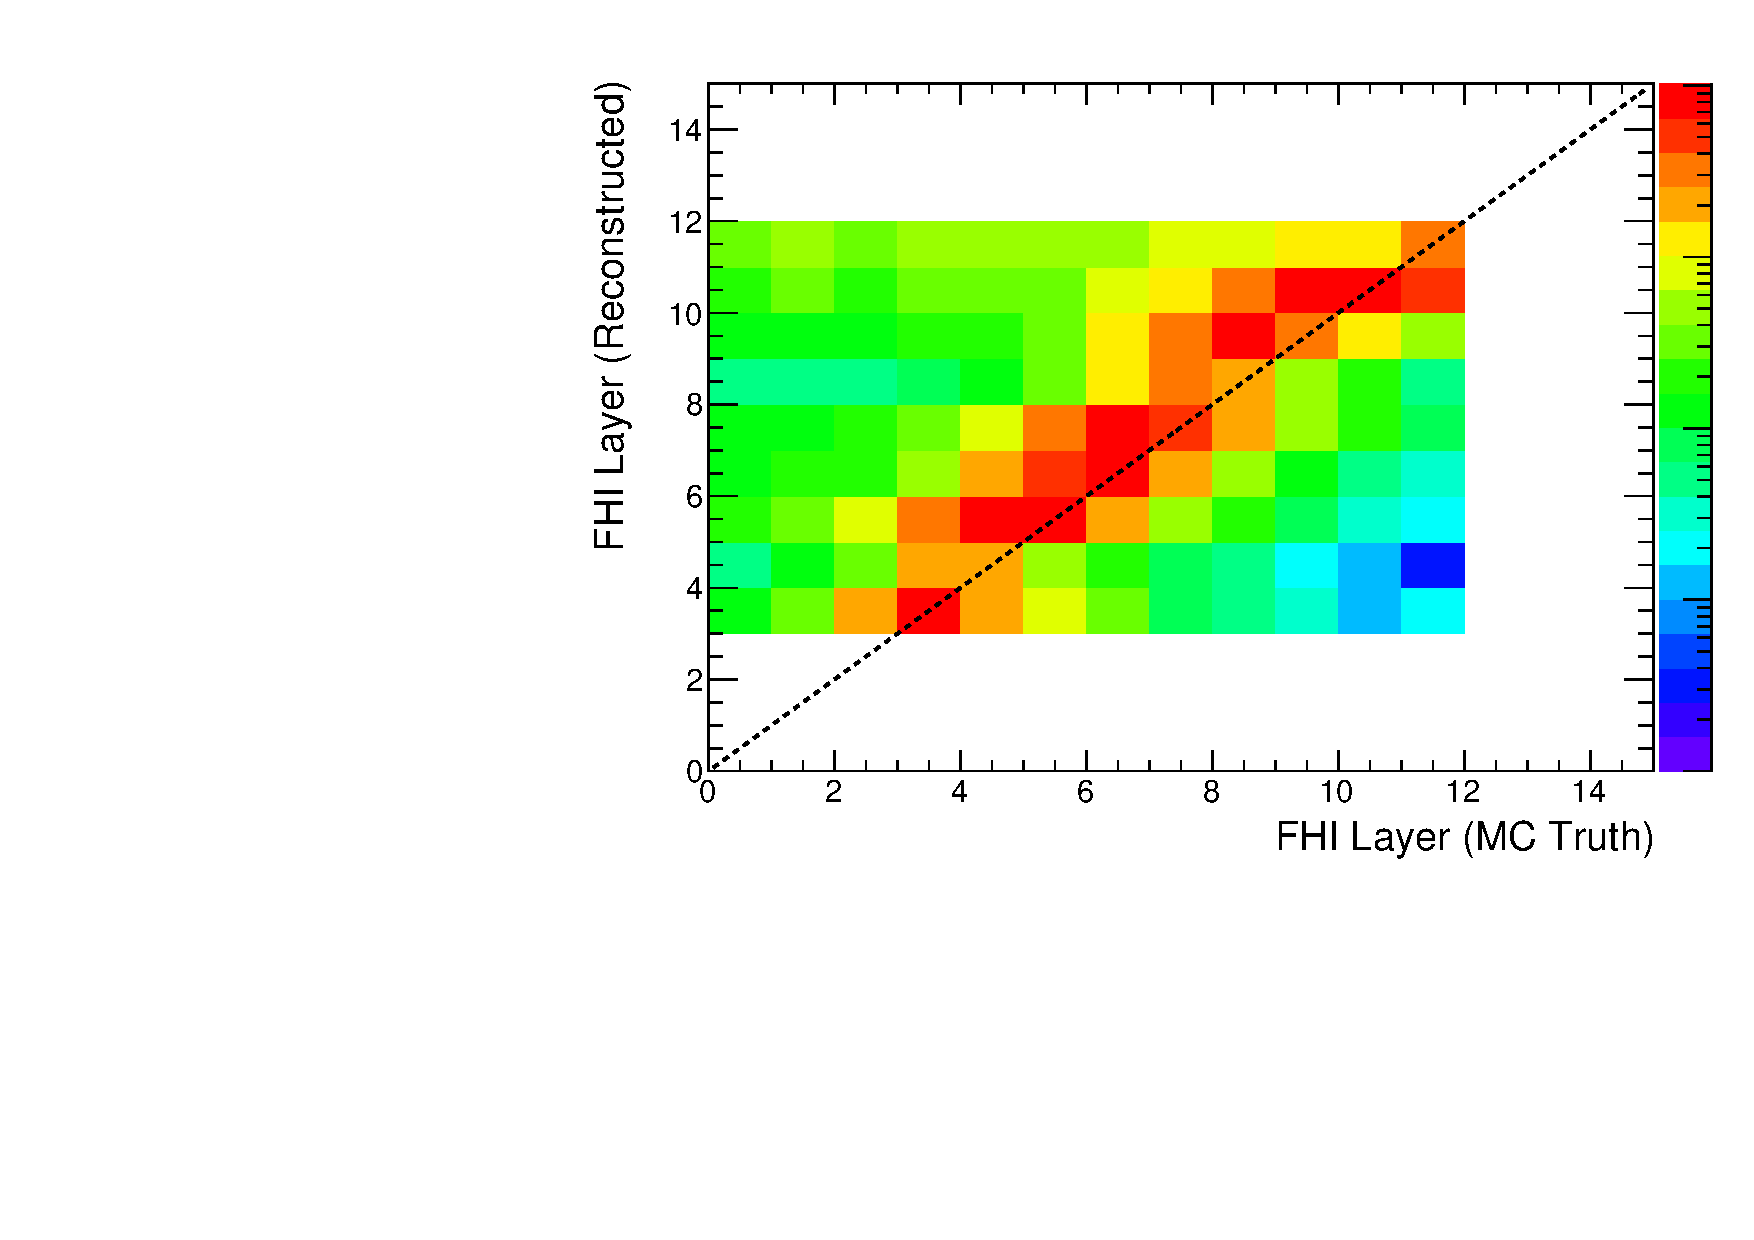
\includegraphics[width=1\textwidth]{../Thesis_Plots/Timing/Pions/Plots/ShowerStart_Difference_noOptimisation_2D.pdf}
		\caption{Correlation between reconstructed FHI and MC truth layer.}\label{fig:Corr_FHI_RecoMC}
	\end{subfigure}
	\caption{Performance check of the FHI algorithm in the AHCAL detector. The left plot shows the difference between the reconstructed FHI and the MC truth. The distribution is slightly decentered at -0.81 with a RMS of 1.87. The right plot shows the correlation between them. The black line represent a guide line for a perfect correlation.}
	\label{fig:FHIAlgo}
\end{figure}

Looking back at the data, it is expected that with a constant distance between the reconstructed FHI and the layer investigated that there will be the same dependence of the mean time of the hit as function of the radius as the same part of the shower is sampled. Or that inversely by looking at a fixed layer for different FHI layer, the expected behavior would be a change in the slope of the time of first hit as function of the radius to the shower axis. The figure \ref{fig:Radius_FHI} and \ref{fig:Radius_FHI_Fixed} is an attempt at this.

\begin{figure}[htbp!]
	\begin{subfigure}[t]{0.5\textwidth}
		\centering
		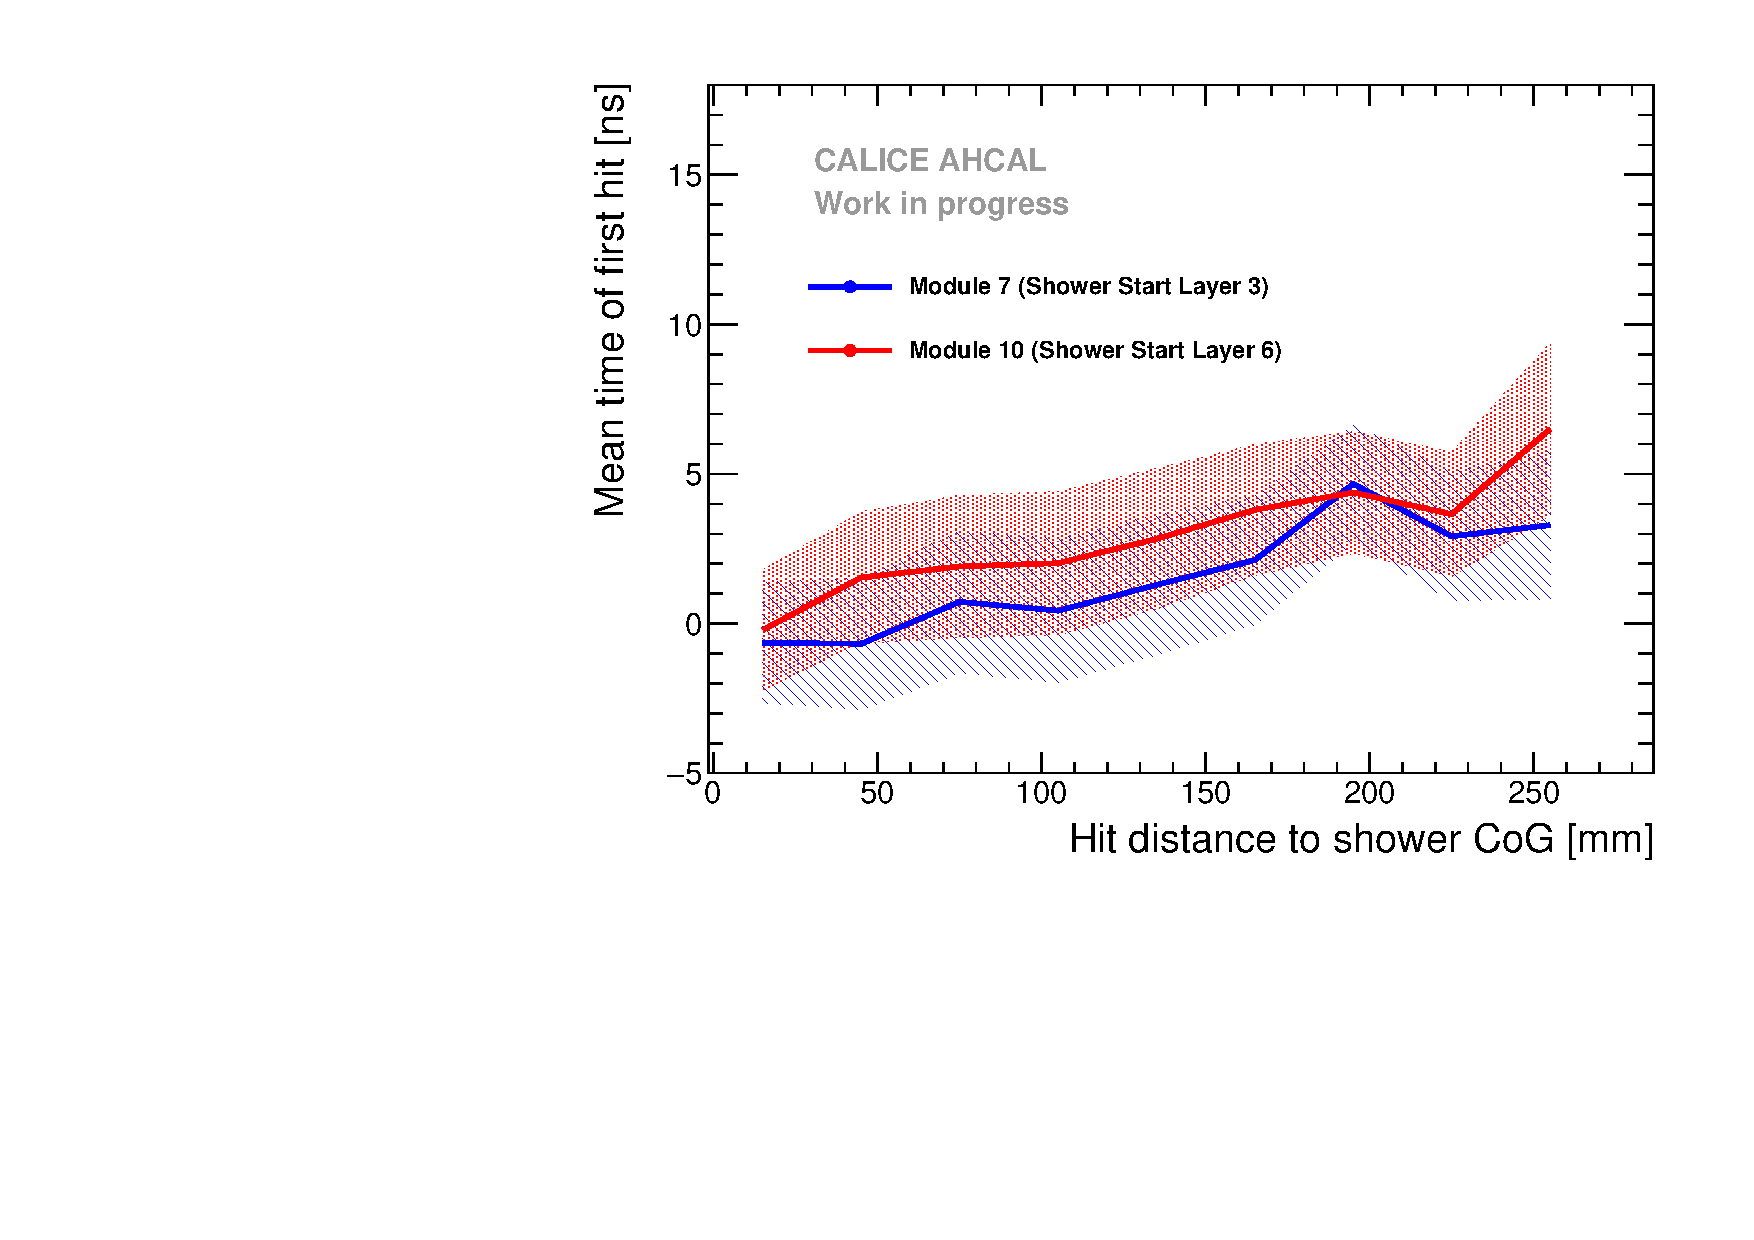
\includegraphics[width=1\textwidth]{../Thesis_Plots/Timing/Pions/Plots/Timing_Radius_Comparison_ShortAsymRange_ShowerStart.pdf}
		\caption{Fixed FHI-layer distance case.}\label{fig:Radius_FHI}
	\end{subfigure}
	\hfill
	\begin{subfigure}[t]{0.5\textwidth}
		\centering
		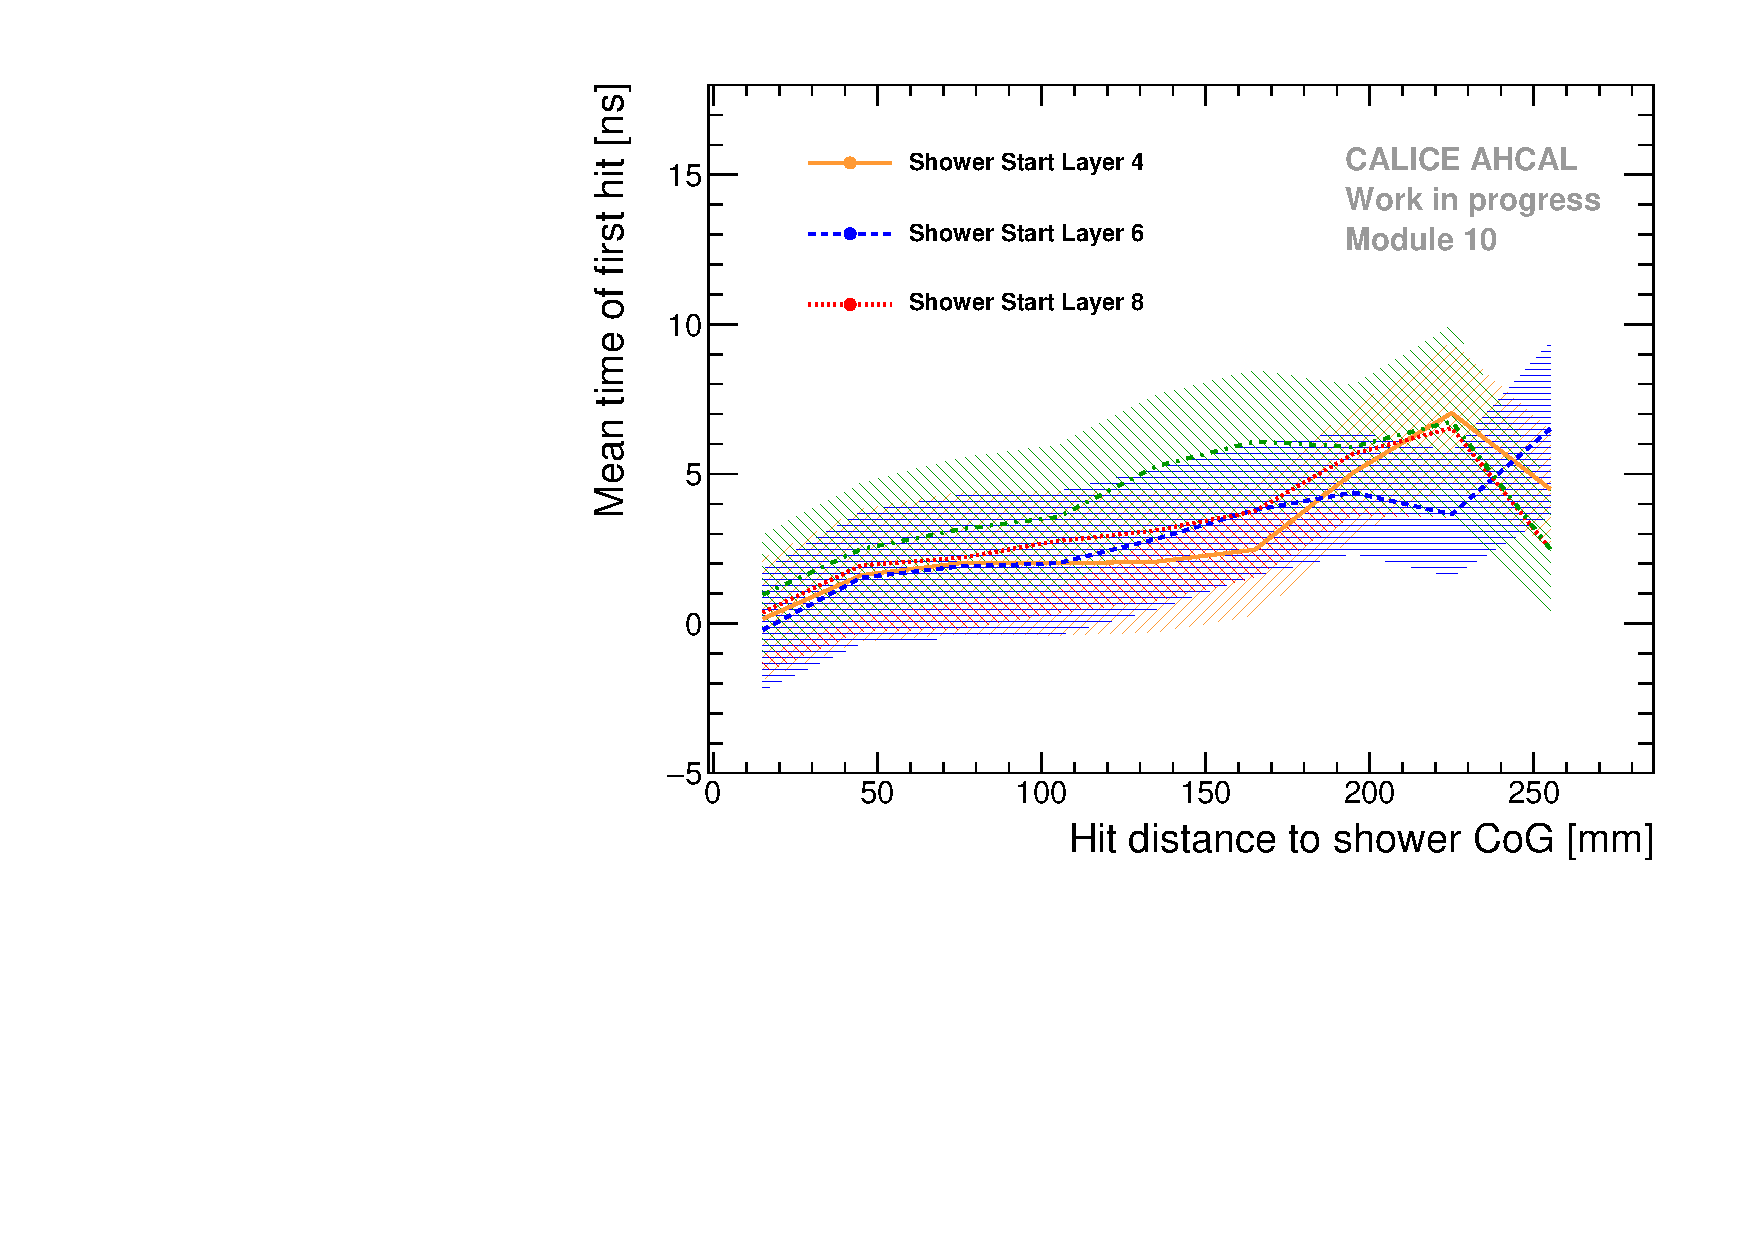
\includegraphics[width=1\textwidth]{../Thesis_Plots/Timing/Pions/Plots/Timing_Radius_Comparison_ShortAsymRange_ShowerStart_FixedModule.pdf}
		\caption{Fixed layer with difference FHI case.}\label{fig:Radius_FHI_Fixed}
	\end{subfigure}
	\caption{Investigation of the difference of the shape of the radial timing distribution between small and big layers. The left plot shows the timing profile of layer 7 and 10 selecting events only where the difference between the reconstructed FHI layer and the observed layer is 4. The right plot shows the time profile of layer 10 for events with different reconstructed FHI.}
	\label{fig:Radius_FHIAll}
\end{figure}

The data seems to shows that by fixing the distance between the FHI and the layer, that the time of first hit displays the same slope within the systematic uncertainties. Also on the other side, looking at a fixed layer in this case layer 10, it seems that there is a trend of an increase of the slope of the distribution as function of the reconstructed FHI within the systematics. But because of many layers not working well, it is difficult to find a comparable configuration to confirm the observation. Also, a reduction of the systematic uncertainty is needed. This also has been checked with simulations as shown in figure \ref{fig:Radius_FHISim}.

\begin{figure}[htbp!]
	\begin{subfigure}[t]{0.5\textwidth}
		\centering
		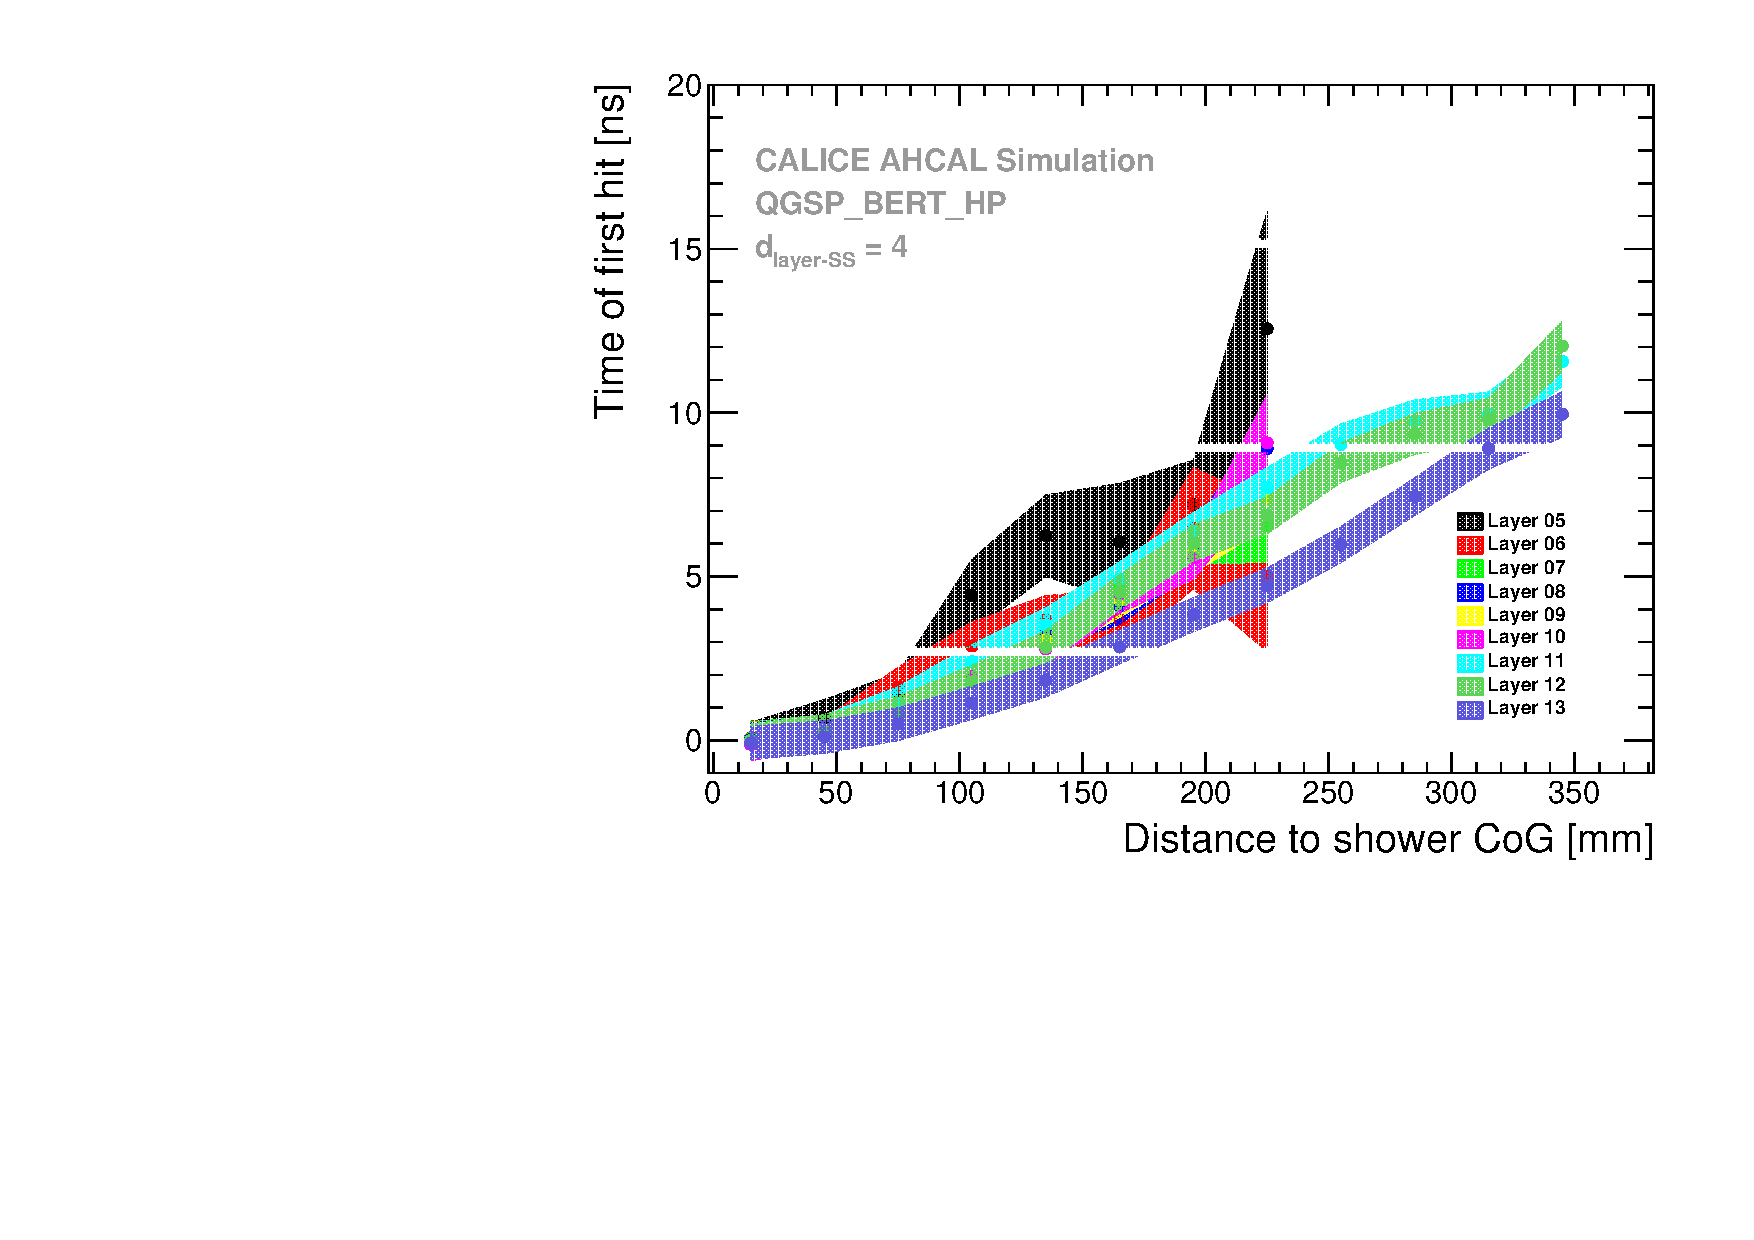
\includegraphics[width=1\textwidth]{../Thesis_Plots/Timing/Pions/Plots/Radius_ShowerStartTruth.pdf}
		\caption{}\label{fig:Radius_FHISim1}
	\end{subfigure}
	\hfill
	\begin{subfigure}[t]{0.5\textwidth}
		\centering
		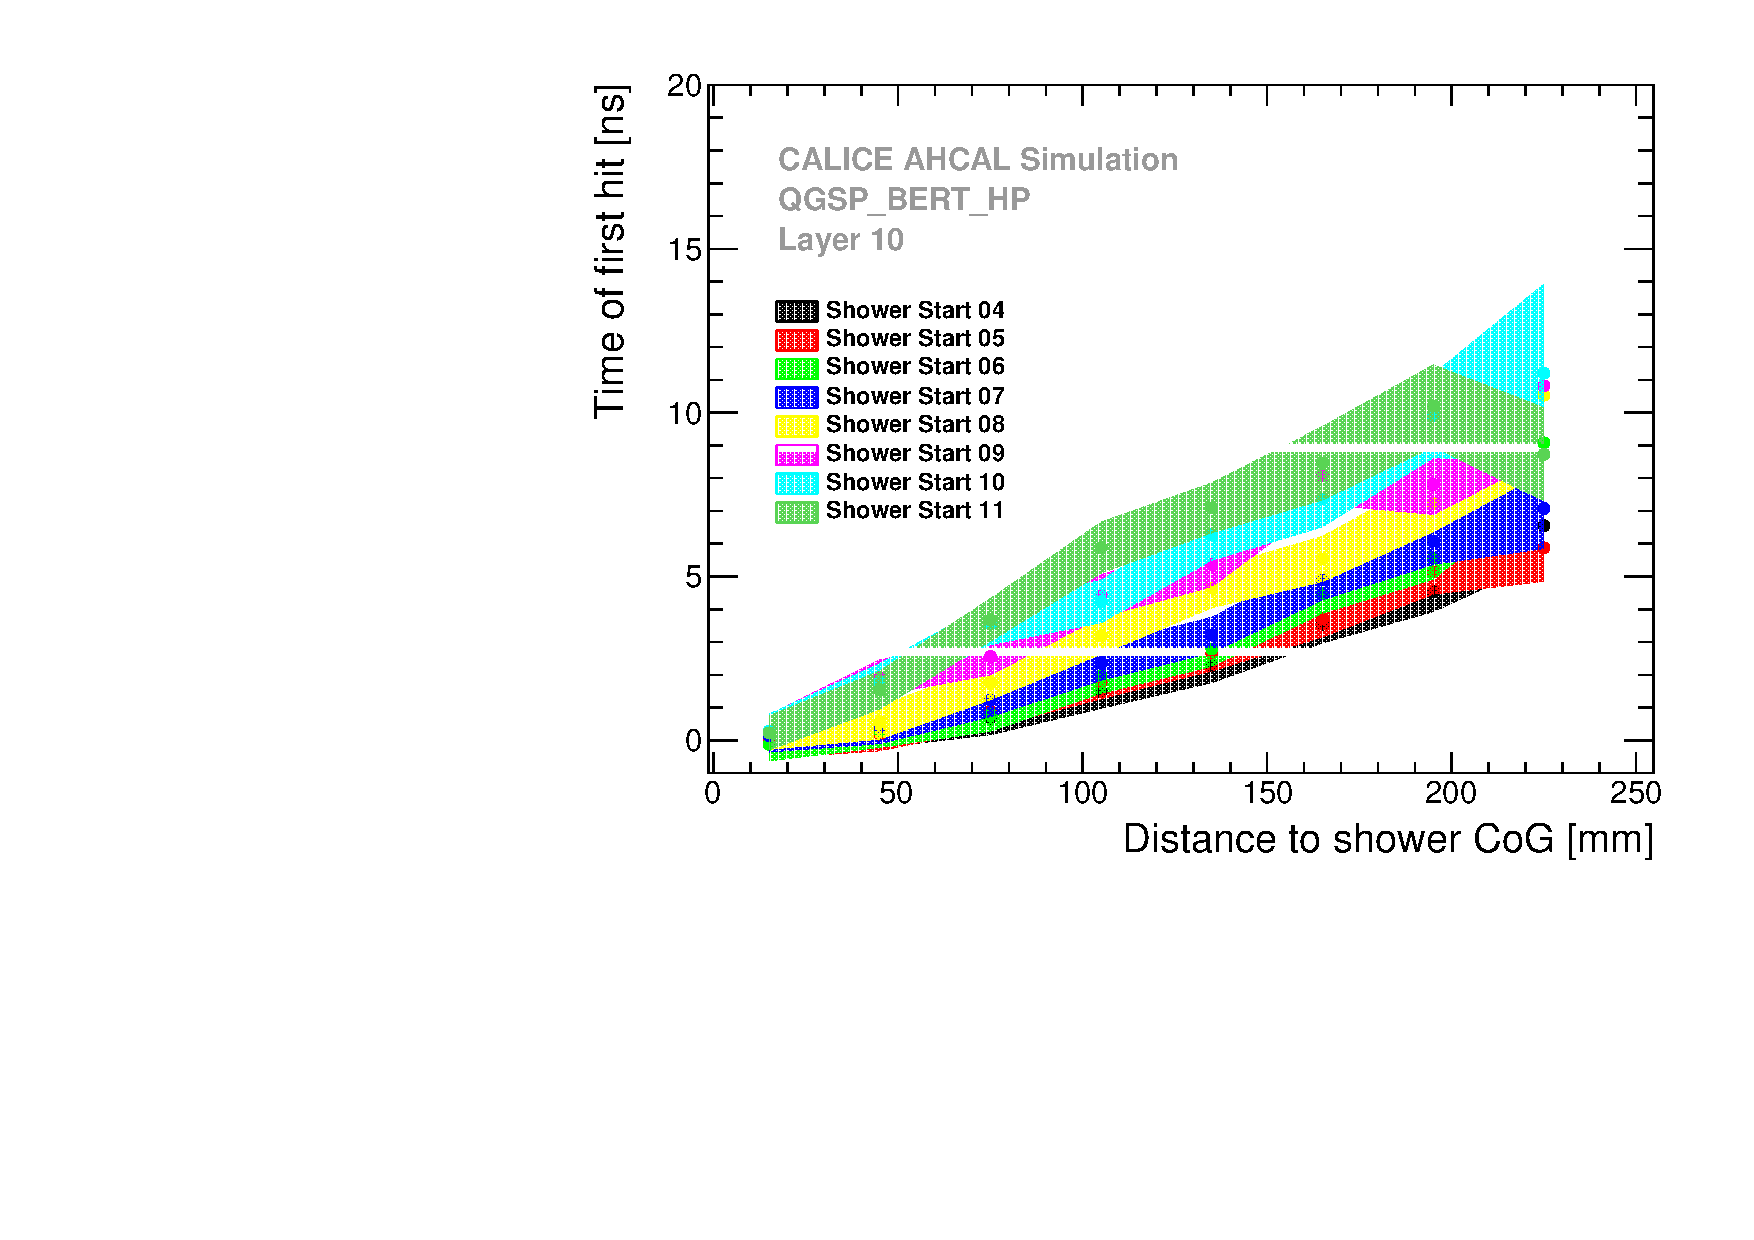
\includegraphics[width=1\textwidth]{../Thesis_Plots/Timing/Pions/Plots/Radius_ShowerStartTruth_FixedModule.pdf}
		\caption{}\label{fig:Radius_FHI_FixedSim}
	\end{subfigure}
	\caption{Time of first hit as function of the hit distance to the center of gravity for 50 GeV pions in \mokka simulation using QGSP\_BERT\_HP. For the left plot, a fixed FHI-layer distance of 4 is used. For the right plot, the layer 10 is investigated for different reconstructed FHI layer.}
	\label{fig:Radius_FHISim}
\end{figure}

To complement this, a dependence of the mean time of first hit as function of the hit distance to the center of gravity of the shower for different layers, corresponding to different shower depths, is shown in figure \ref{fig:Radius_Indivi}.
One can observe that there is a dependence of the slope as function of the layer. The layer 3 shows a much steeper slope than for the layer 14. This dependence is not fully understood at the moment and seems counter intuitive as one would expect more later hits in the last layers. One possibility that the later component for the first layers could come from the Albedo effect \cite{ELLSWORTH1982167} and backscattered neutrons. It has been studied in simulation also with the QGSP\_BERT\_HP physics list and the same behavior is described by the simulation as shown in figure \ref{fig:Radius_Indivi_Sim}.

\begin{figure}[htbp!]
	\begin{subfigure}[t]{0.5\textwidth}
		\centering
		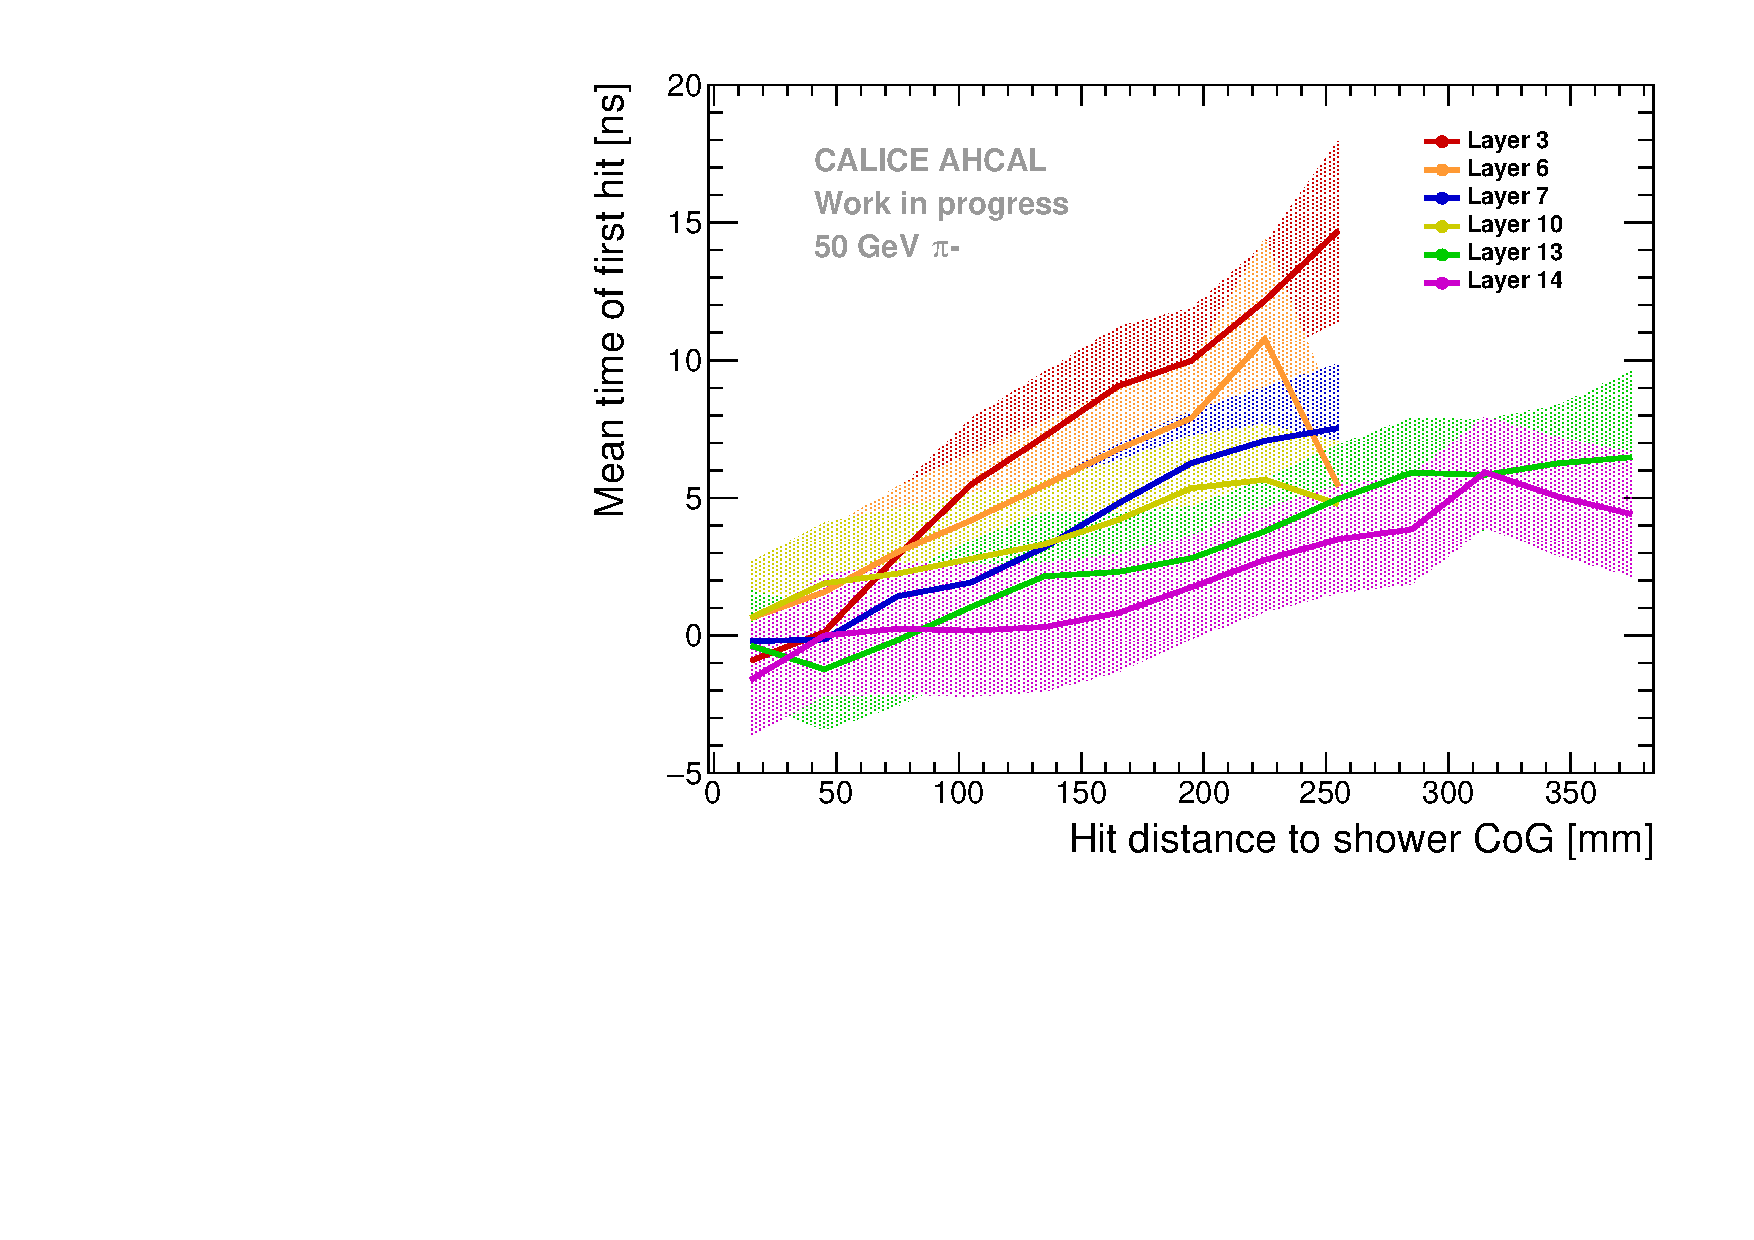
\includegraphics[width=1\textwidth]{../Thesis_Plots/Timing/Pions/Plots/Timing_Radius_Comparison_ShortAsymRange_IndividualLayers.pdf}
		\caption{}\label{fig:Radius_Indivi}
	\end{subfigure}
	\hfill
	\begin{subfigure}[t]{0.5\textwidth}
		\centering
		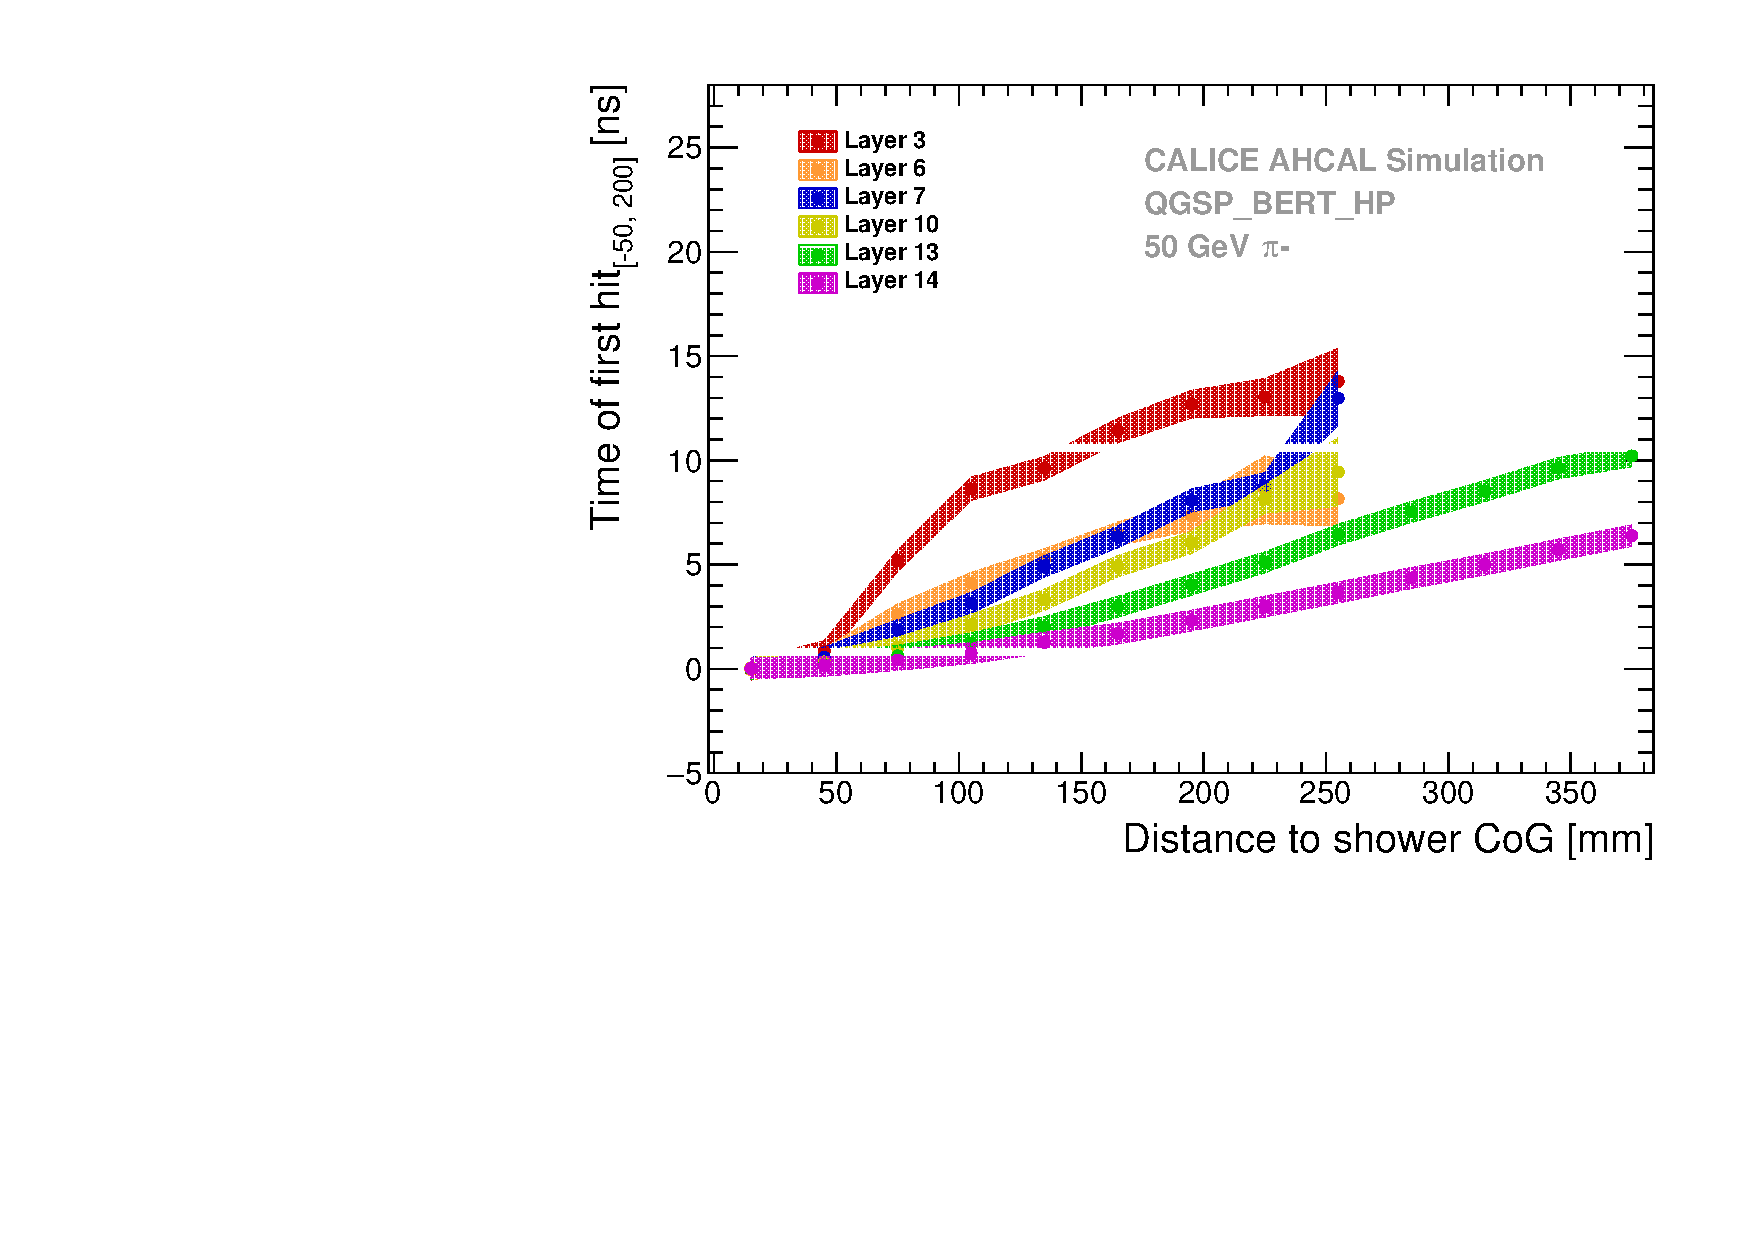
\includegraphics[width=1\textwidth]{../Thesis_Plots/Timing/Pions/Plots/Timing_Radius_Comparison_ShortAsymRange_IndividualLayers_Sim.pdf}
		\caption{}\label{fig:Radius_Indivi_Sim}
	\end{subfigure}
	\caption{Time of first hit as function of the hit distance to the center of gravity for 50 GeV pions. For the left plot, it is shown for data. On the right plot, it is shown for \mokka simulation using QGSP\_BERT\_HP physics list. Both figures shows the same behavior.}
	\label{fig:Radius_IndiviAll}
\end{figure}

The radial profile of pion showers is also compared to simulations as shown in figures \ref{fig:Radius_SSF_SimData_Comparison} and \ref{fig:Radius_BL_SimData_Comparison}. For the small layers, the physics lists QBBC and QGSP\_BERT\_HP reproduce well the data within systematics. QGSP\_BERT agrees well under 10 cm and starts to deviate up to 4-6 ns at 23 cm. Concerning the big layers, over the full energy range, QGSP\_BERT\_HP physics list agrees the best with the data. QBBC and QGSP\_BERT agree with data up to around 10 cm radius and then lie above the data for the mean time of first hit. The difference with the data varies between few ns to 3-4 ns between 17 cm to 35 cm radius. This confirms that without precision neutron tracking, too many late energy depositions are created that are spread far away from the shower axis.

\begin{figure}[htbp!]
	\begin{subfigure}[t]{0.5\textwidth}
		\centering
		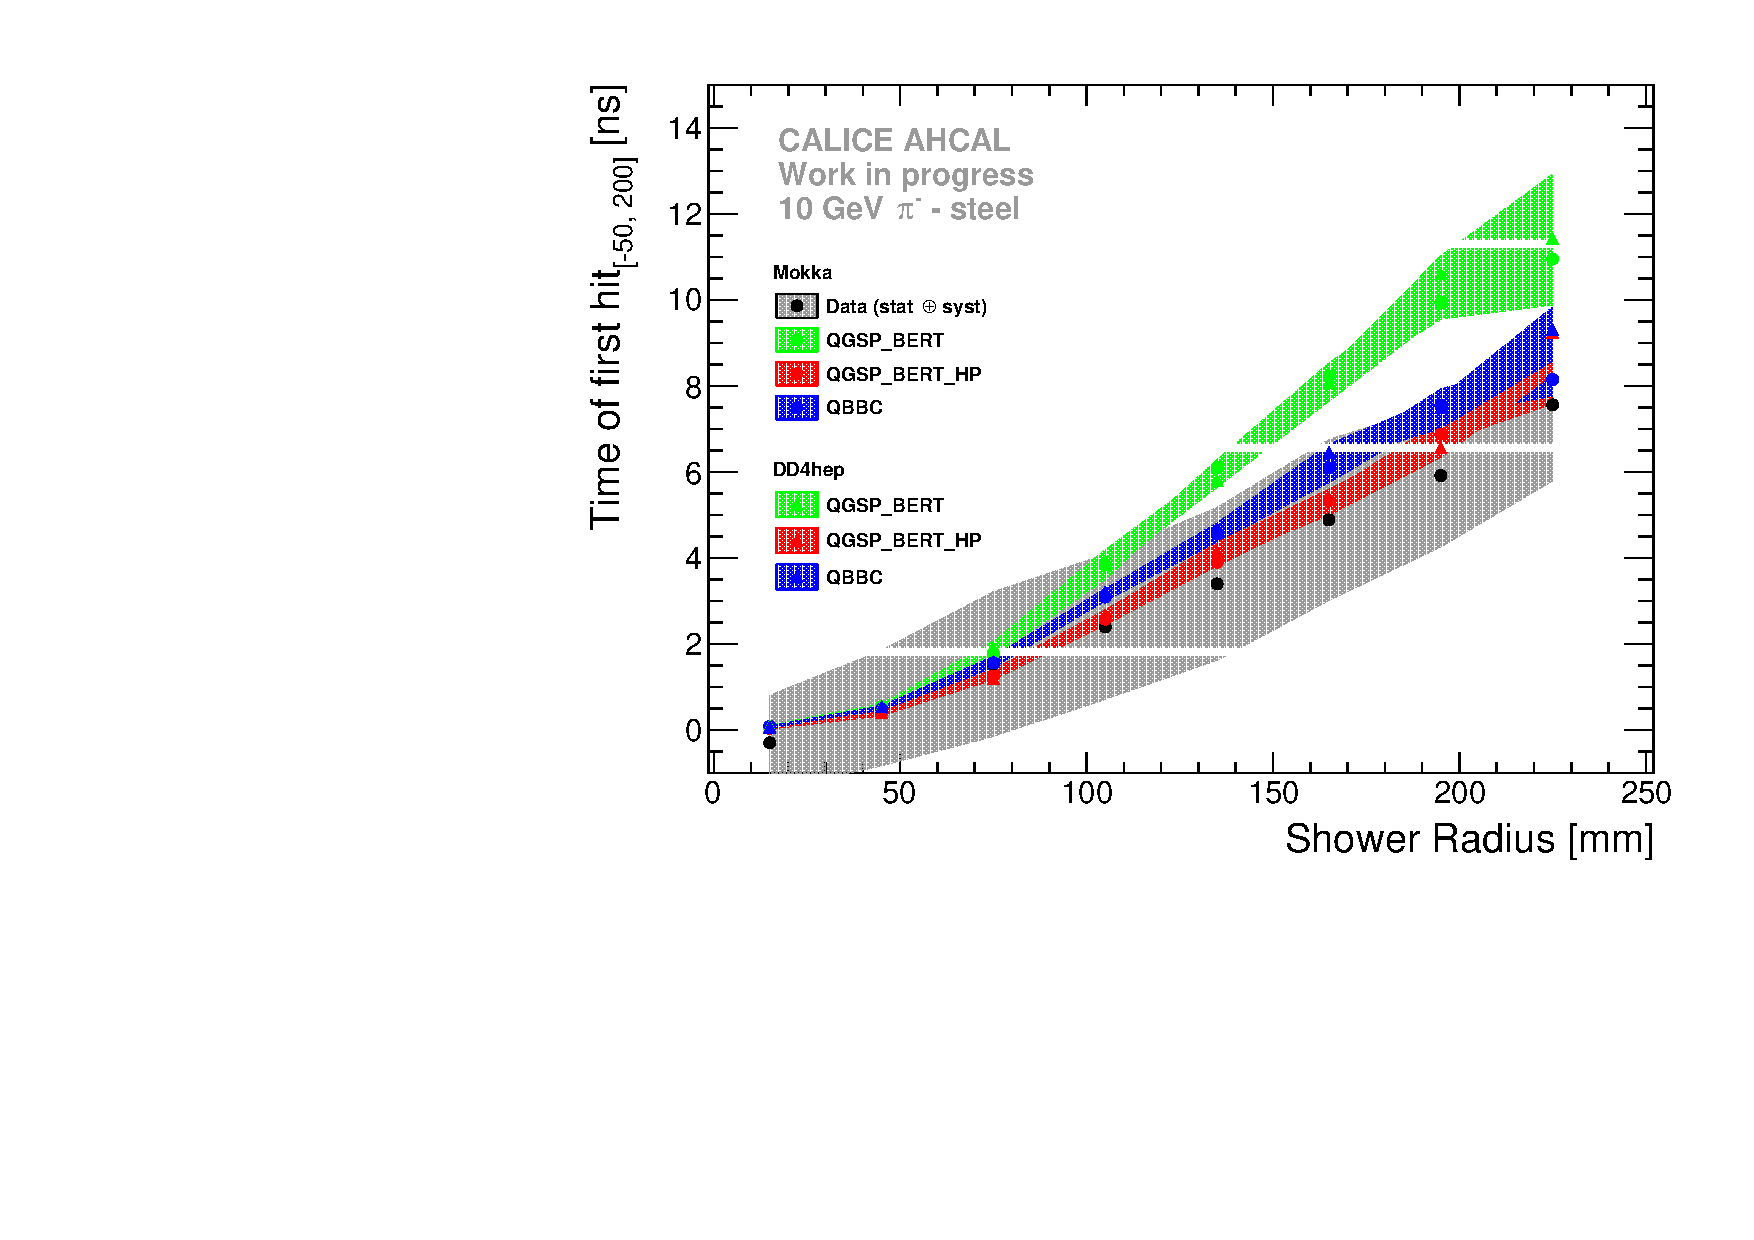
\includegraphics[width=1\textwidth]{../Thesis_Plots/Timing/Pions/Plots/ComparisonToSim/Time_Radius_10GeV_SSF.pdf}
		\caption{10 GeV (SSF).} \label{fig:Radius_SSF_SimData_10GeV}
	\end{subfigure}
	\hfill
	\begin{subfigure}[t]{0.5\textwidth}
		\centering
		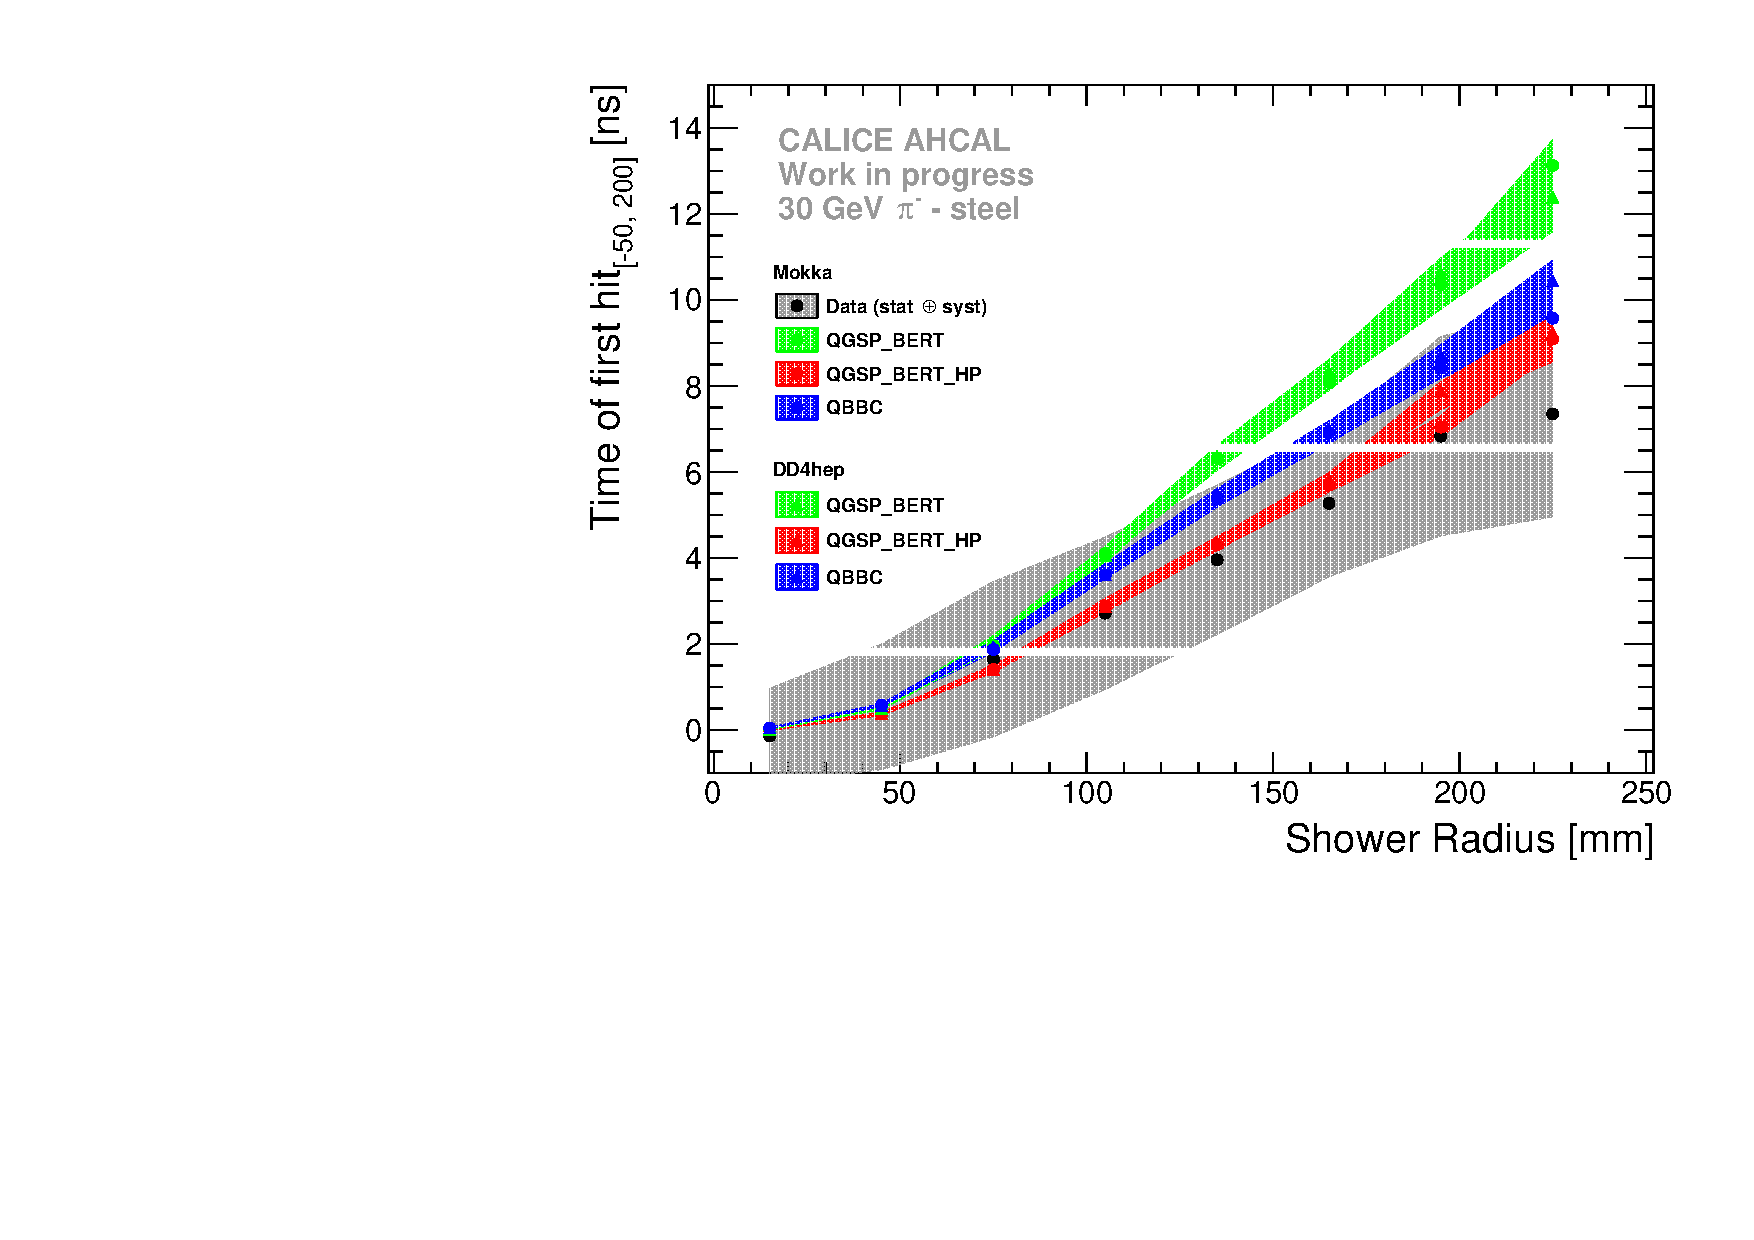
\includegraphics[width=1\textwidth]{../Thesis_Plots/Timing/Pions/Plots/ComparisonToSim/Time_Radius_30GeV_SSF.pdf}
		\caption{30 GeV (SSF).} \label{fig:Radius_SSF_SimData_30GeV}
	\end{subfigure}
	\hfill
	\begin{subfigure}[t]{0.5\textwidth}
		\centering
		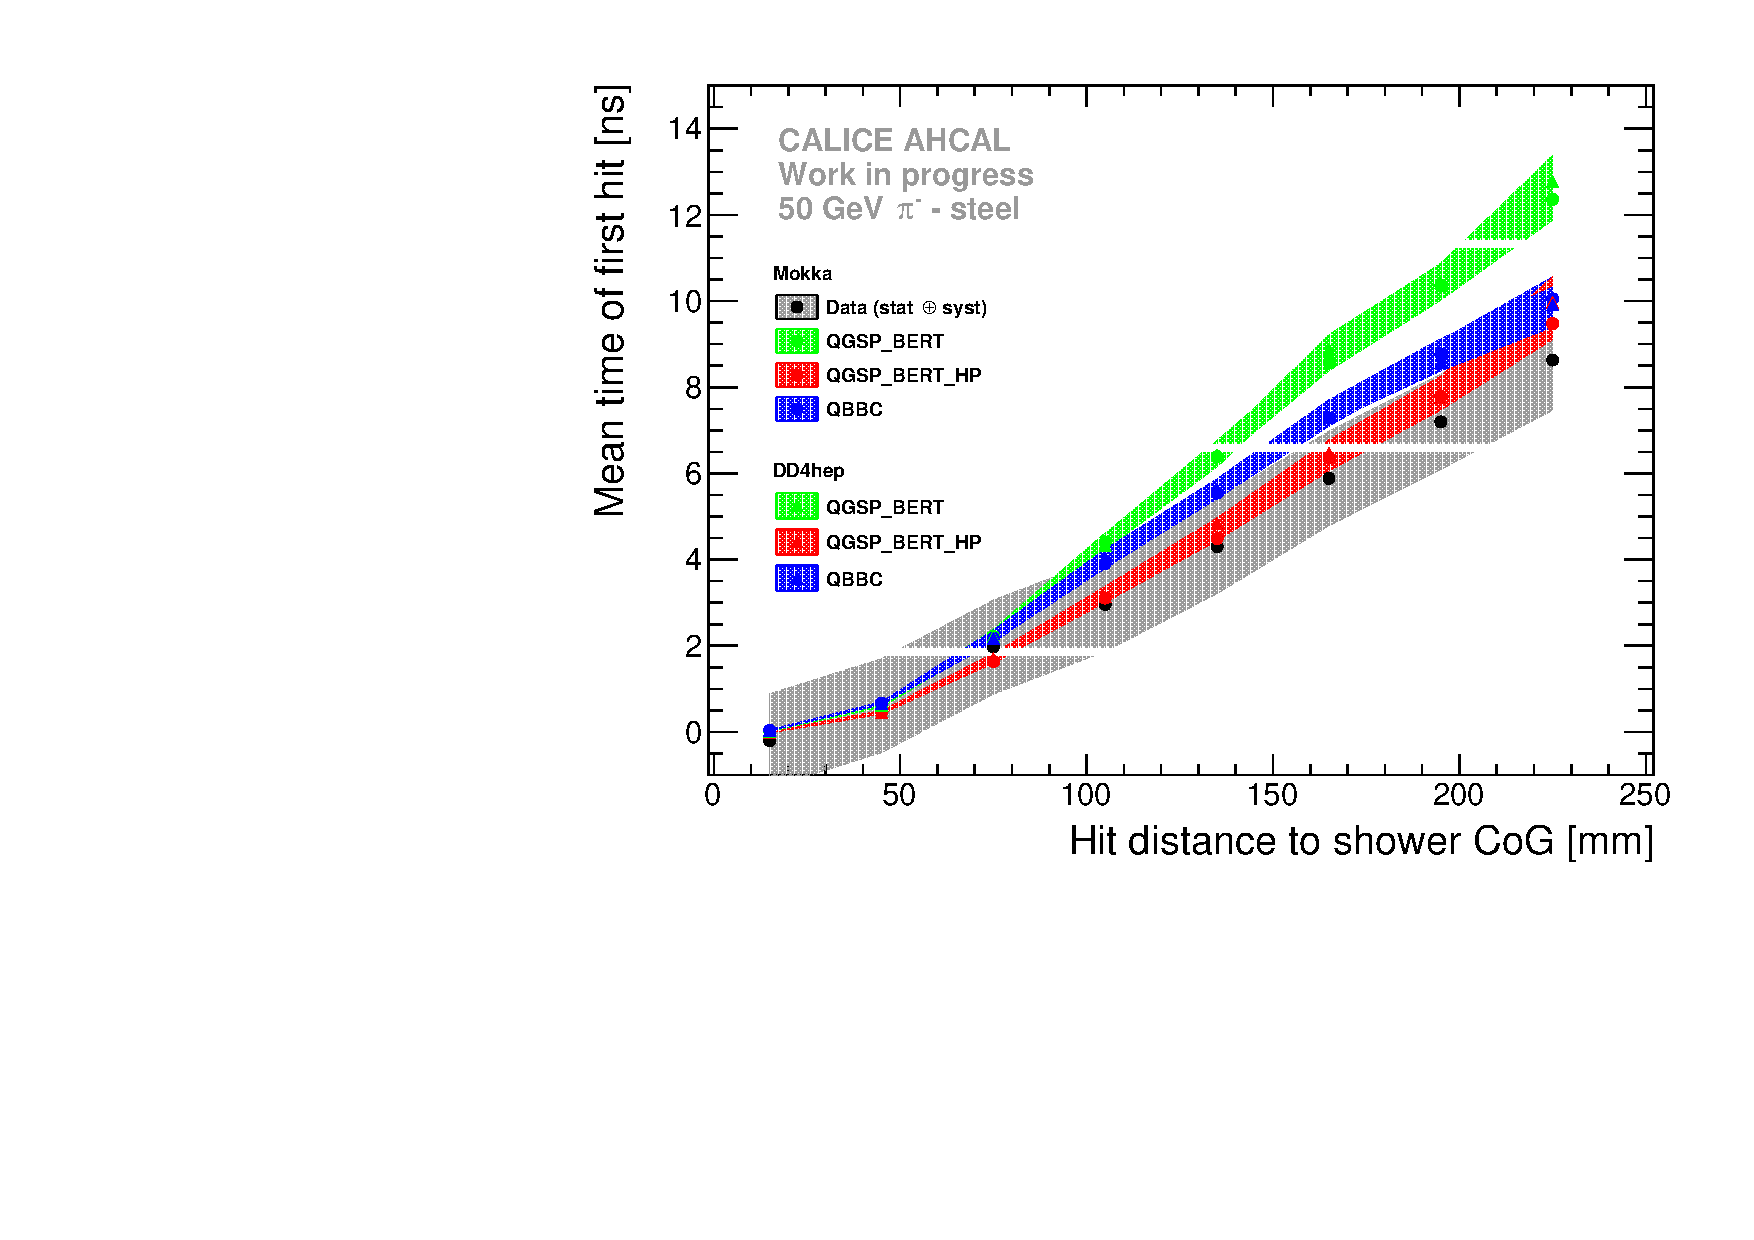
\includegraphics[width=1\textwidth]{../Thesis_Plots/Timing/Pions/Plots/ComparisonToSim/Time_Radius_50GeV_SSF.pdf}
		\caption{50 GeV (SSF).} \label{fig:Radius_SSF_SimData_50GeV}
	\end{subfigure}
	\hfill
	\begin{subfigure}[t]{0.5\textwidth}
		\centering
		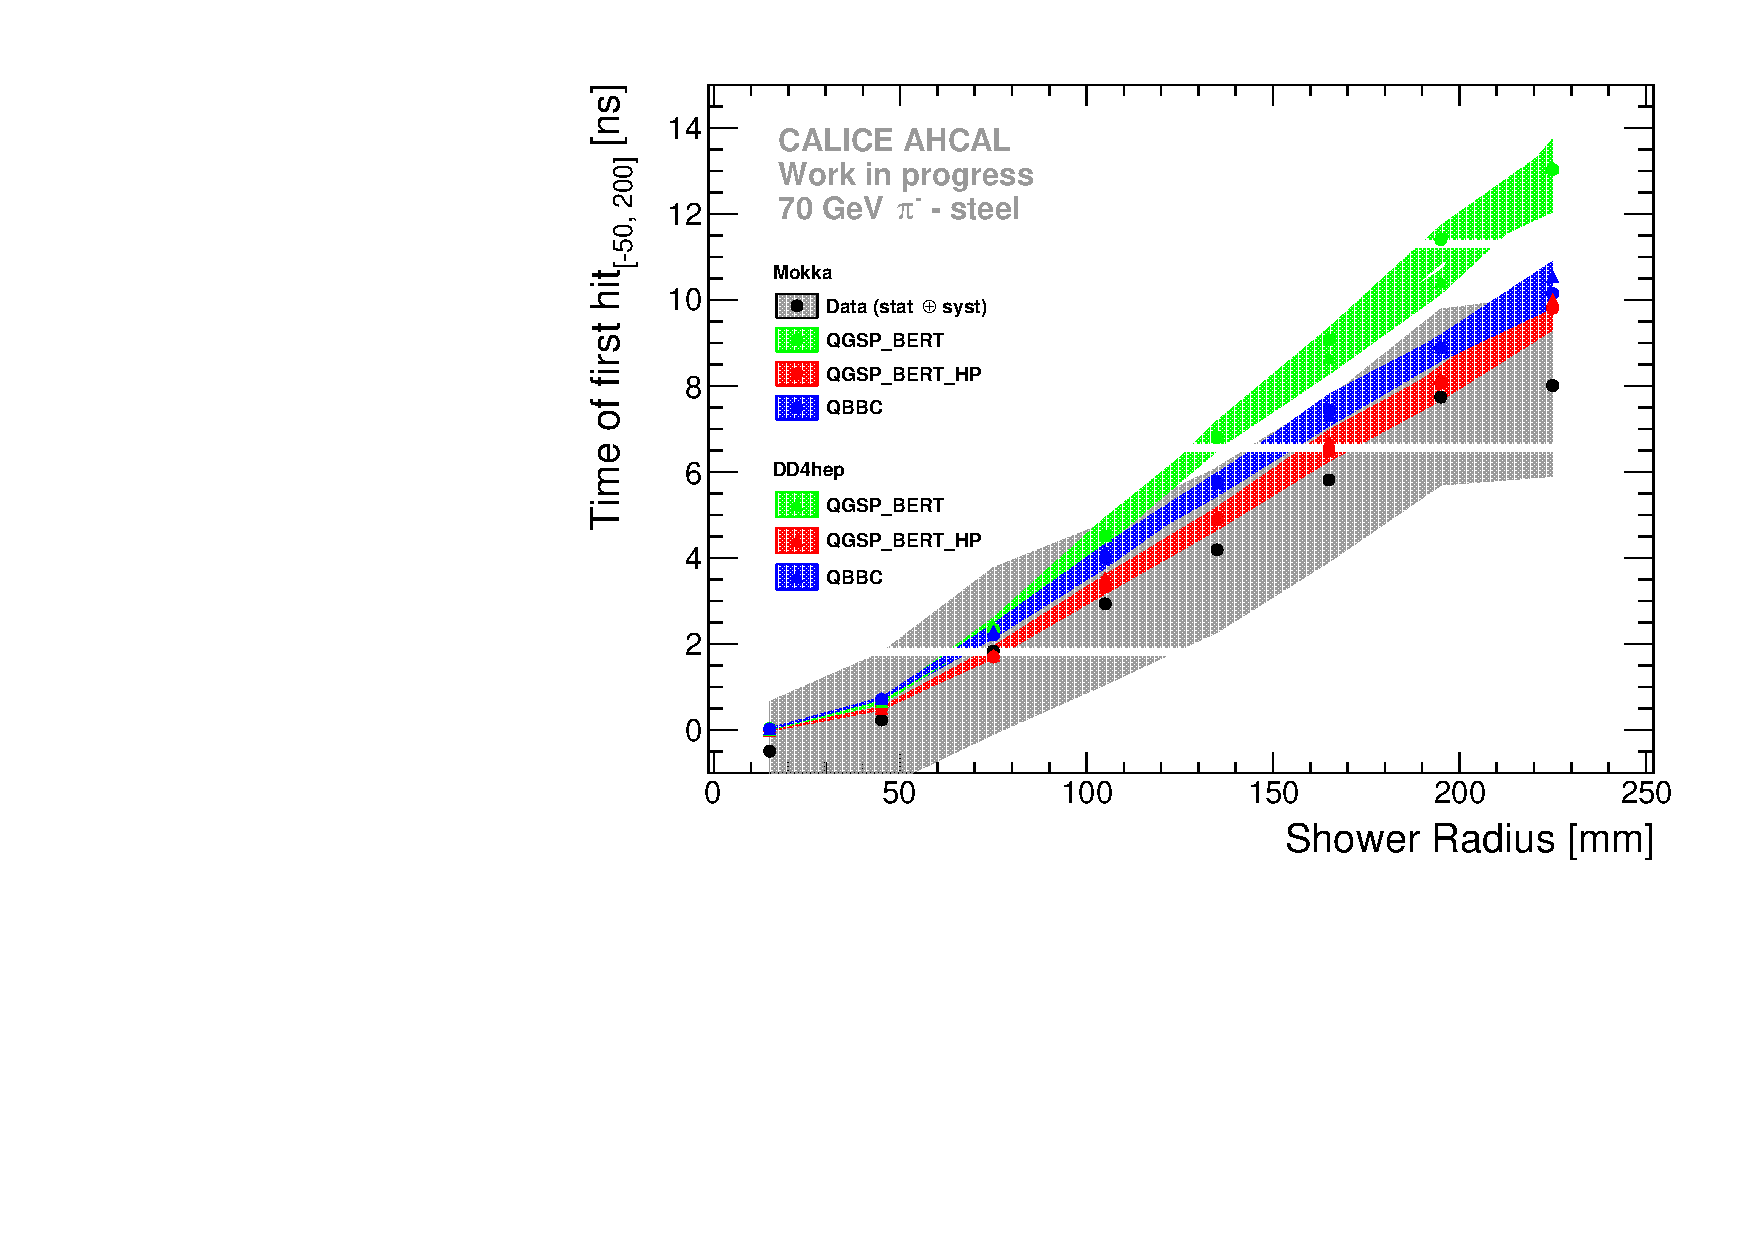
\includegraphics[width=1\textwidth]{../Thesis_Plots/Timing/Pions/Plots/ComparisonToSim/Time_Radius_70GeV_SSF.pdf}
		\caption{70 GeV (SSF).} \label{fig:Radius_SSF_SimData_70GeV}
	\end{subfigure}
	\hfill
	\begin{subfigure}[t]{0.5\textwidth}
		\centering
		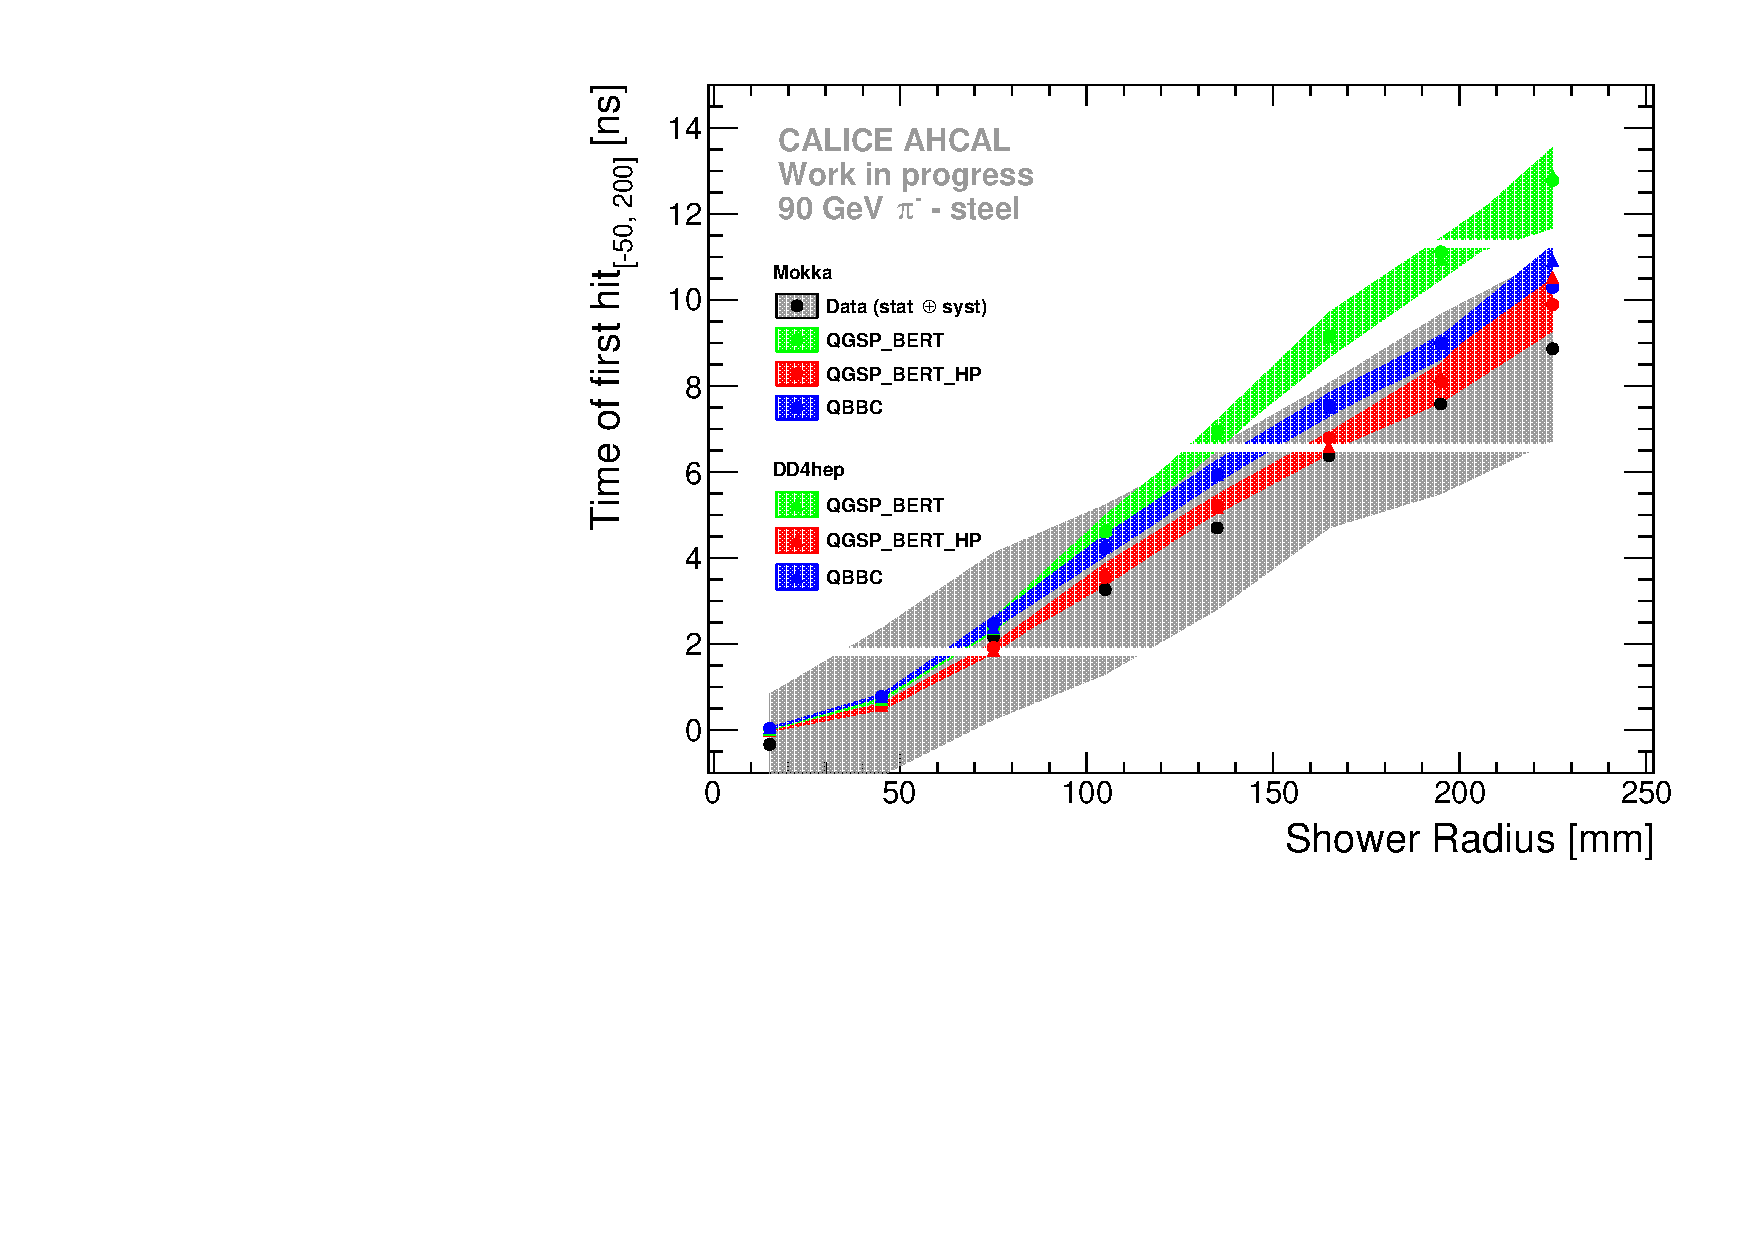
\includegraphics[width=1\textwidth]{../Thesis_Plots/Timing/Pions/Plots/ComparisonToSim/Time_Radius_90GeV_SSF.pdf}
		\caption{90 GeV (SSF).} \label{fig:Radius_SSF_SimData_90GeV}
	\end{subfigure}
	\caption{Comparison between simulations and data of the time of first hit as function of the distance to the shower axis for pion beams between 10 GeV and 90 GeV for the small layers (layers 3 to 10). The grey and color bands shows the systematics.}
	\label{fig:Radius_SSF_SimData_Comparison}
\end{figure}

\begin{figure}[htbp!]
	\begin{subfigure}[t]{0.5\textwidth}
		\centering
		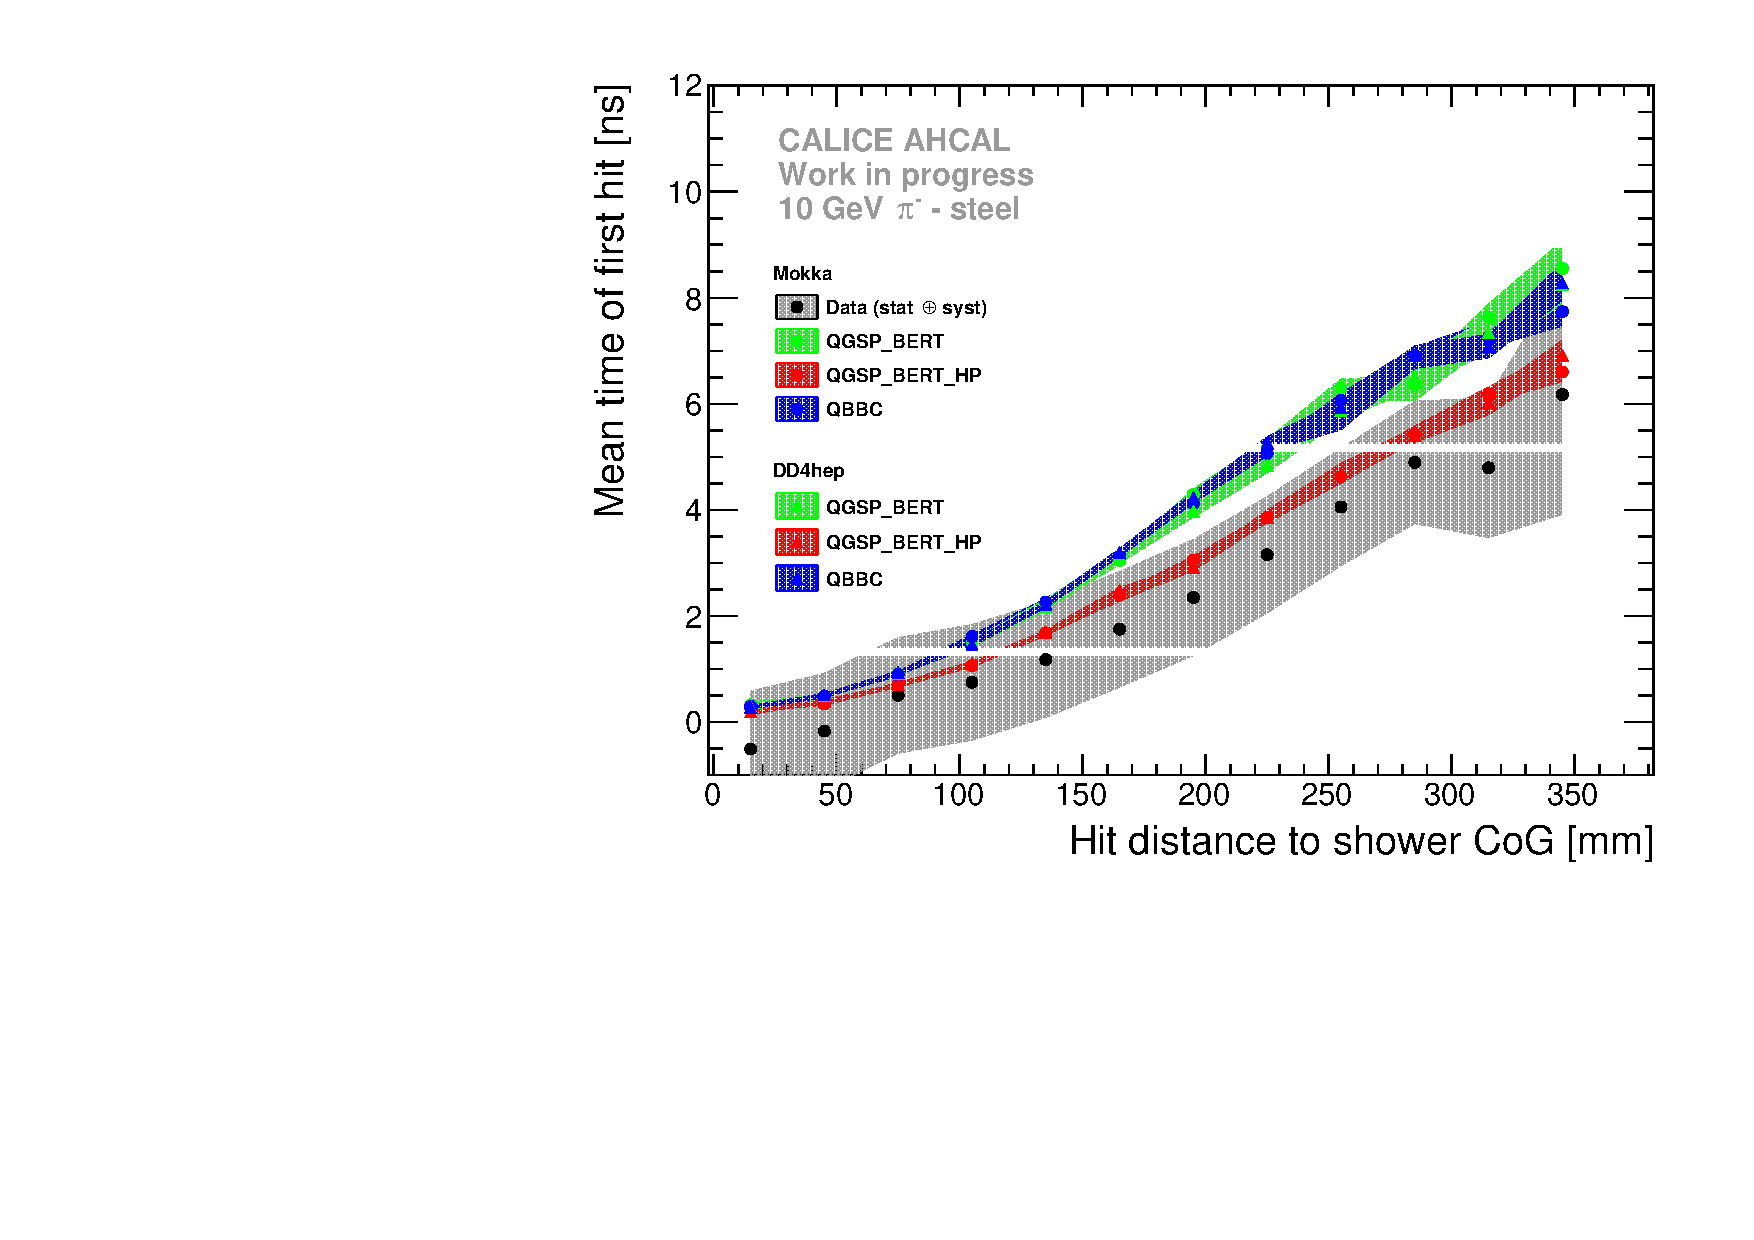
\includegraphics[width=1\textwidth]{../Thesis_Plots/Timing/Pions/Plots/ComparisonToSim/Time_Radius_10GeV_BL.pdf}
		\caption{10 GeV (BL).}\label{fig:Radius_BL_SimData_10GeV}
	\end{subfigure}
	\hfill
	\begin{subfigure}[t]{0.5\textwidth}
		\centering
		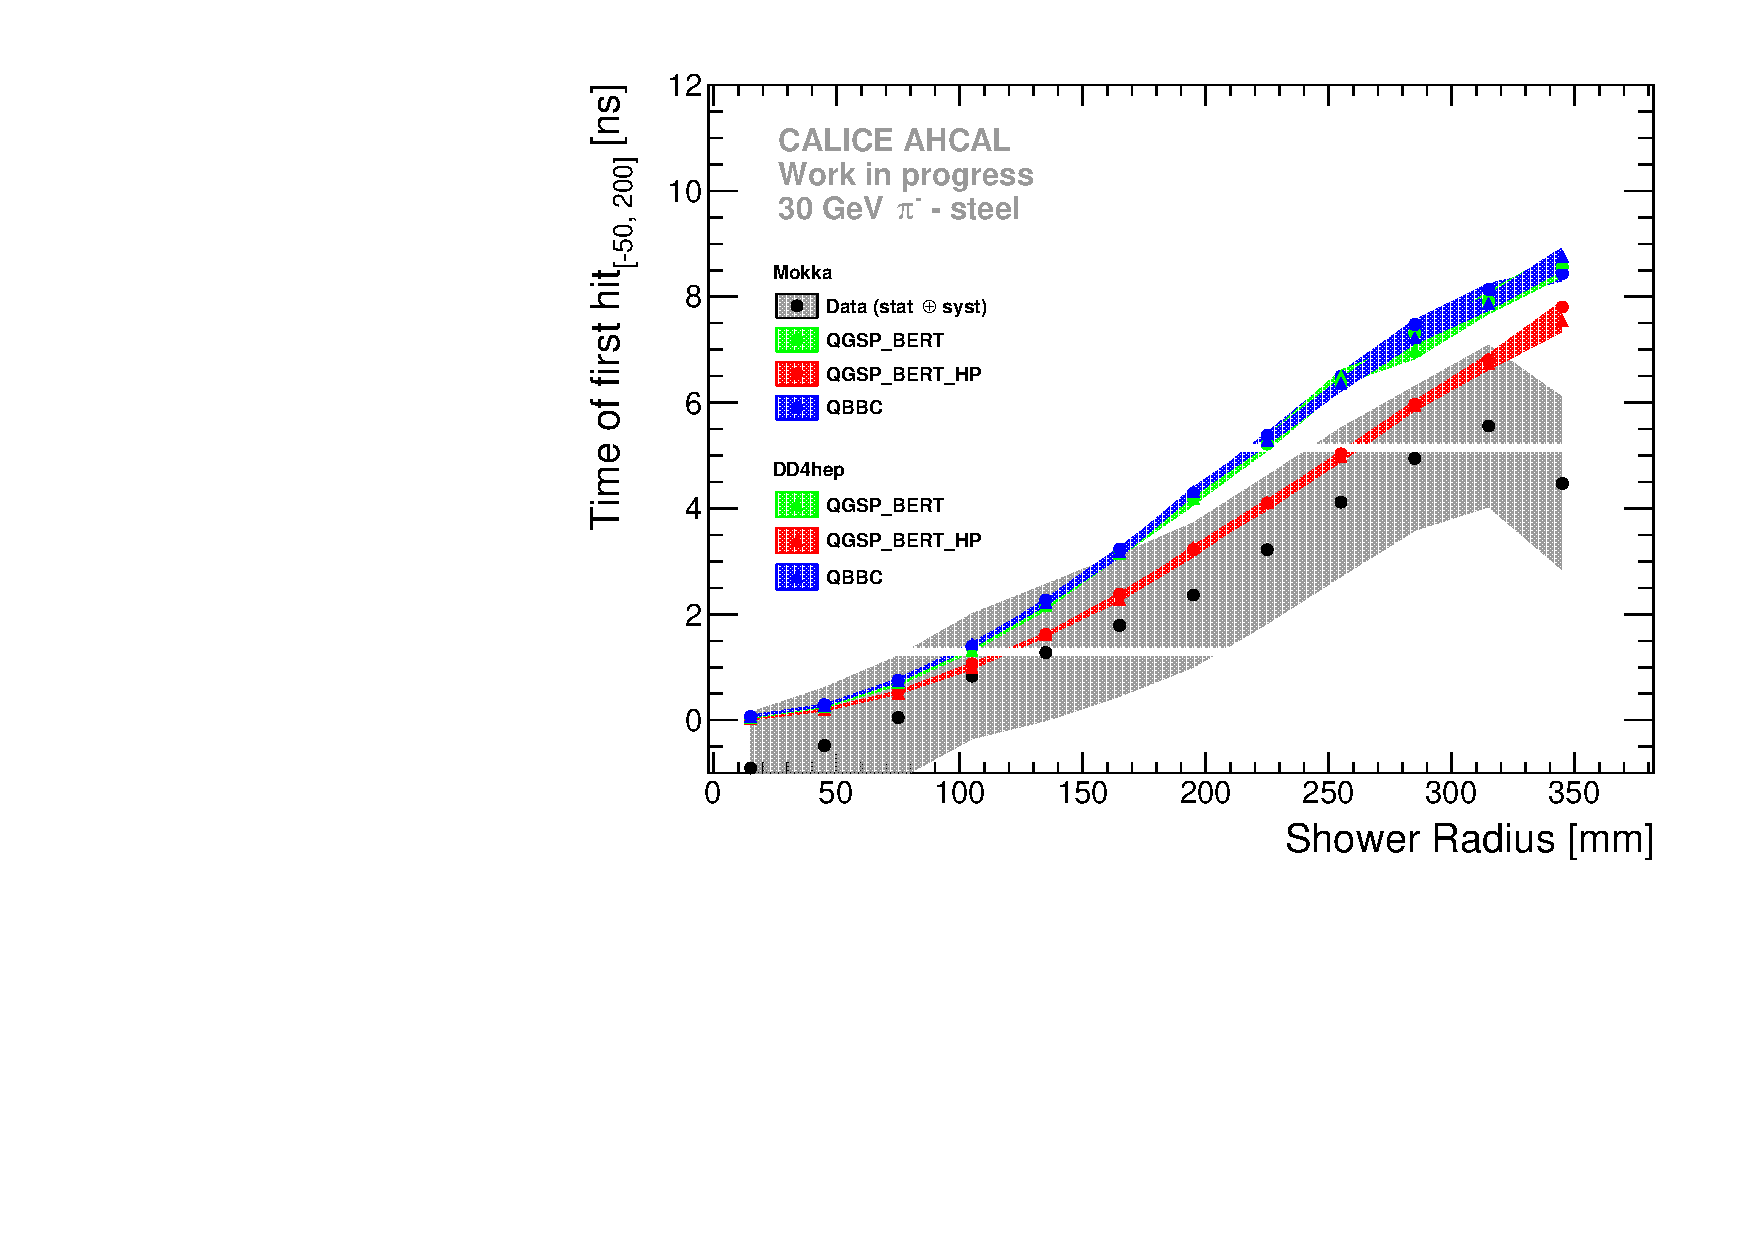
\includegraphics[width=1\textwidth]{../Thesis_Plots/Timing/Pions/Plots/ComparisonToSim/Time_Radius_30GeV_BL.pdf}
		\caption{30 GeV (BL).} \label{fig:Radius_BL_SimData_30GeV}
	\end{subfigure}
	\hfill
	\begin{subfigure}[t]{0.5\textwidth}
		\centering
		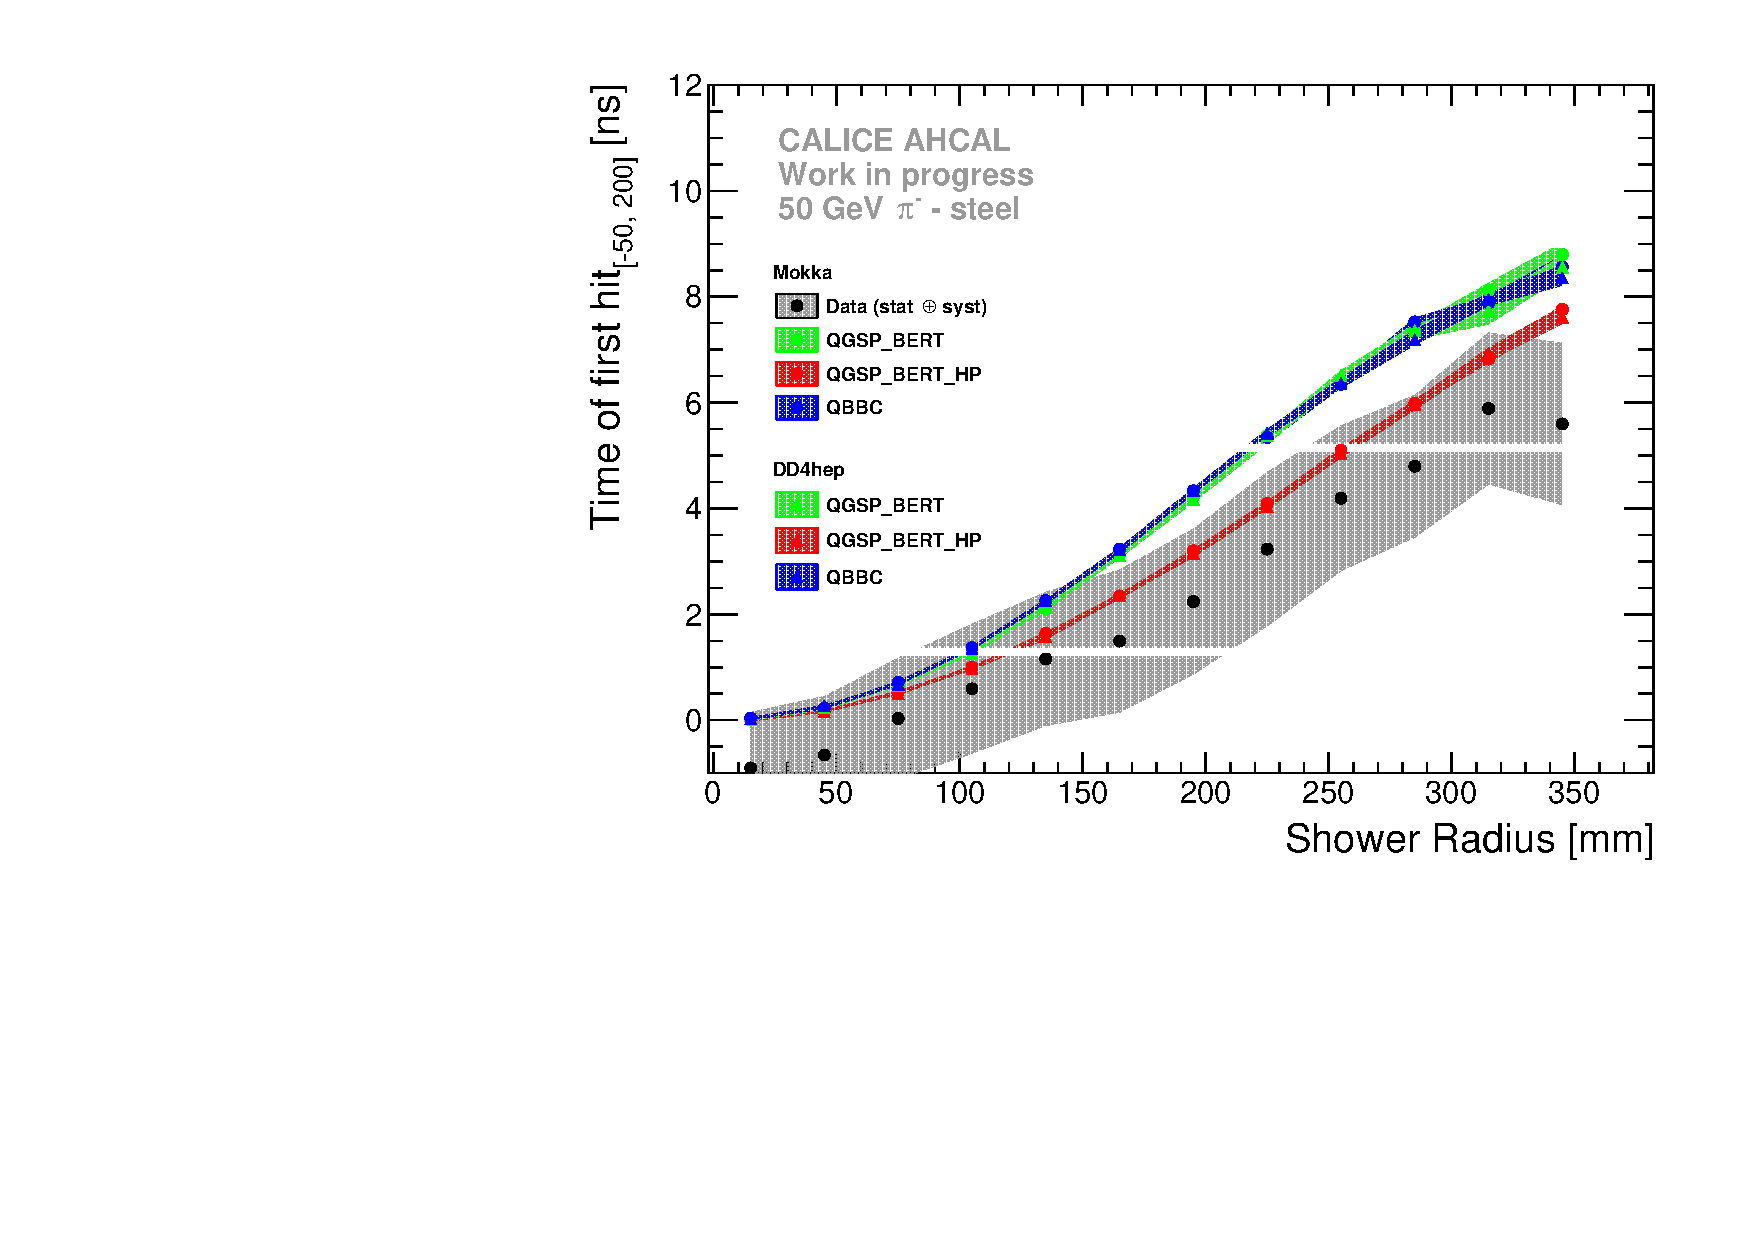
\includegraphics[width=1\textwidth]{../Thesis_Plots/Timing/Pions/Plots/ComparisonToSim/Time_Radius_50GeV_BL.pdf}
		\caption{50 GeV (BL).} \label{fig:Radius_BL_SimData_50GeV}
	\end{subfigure}
	\hfill
	\begin{subfigure}[t]{0.5\textwidth}
		\centering
		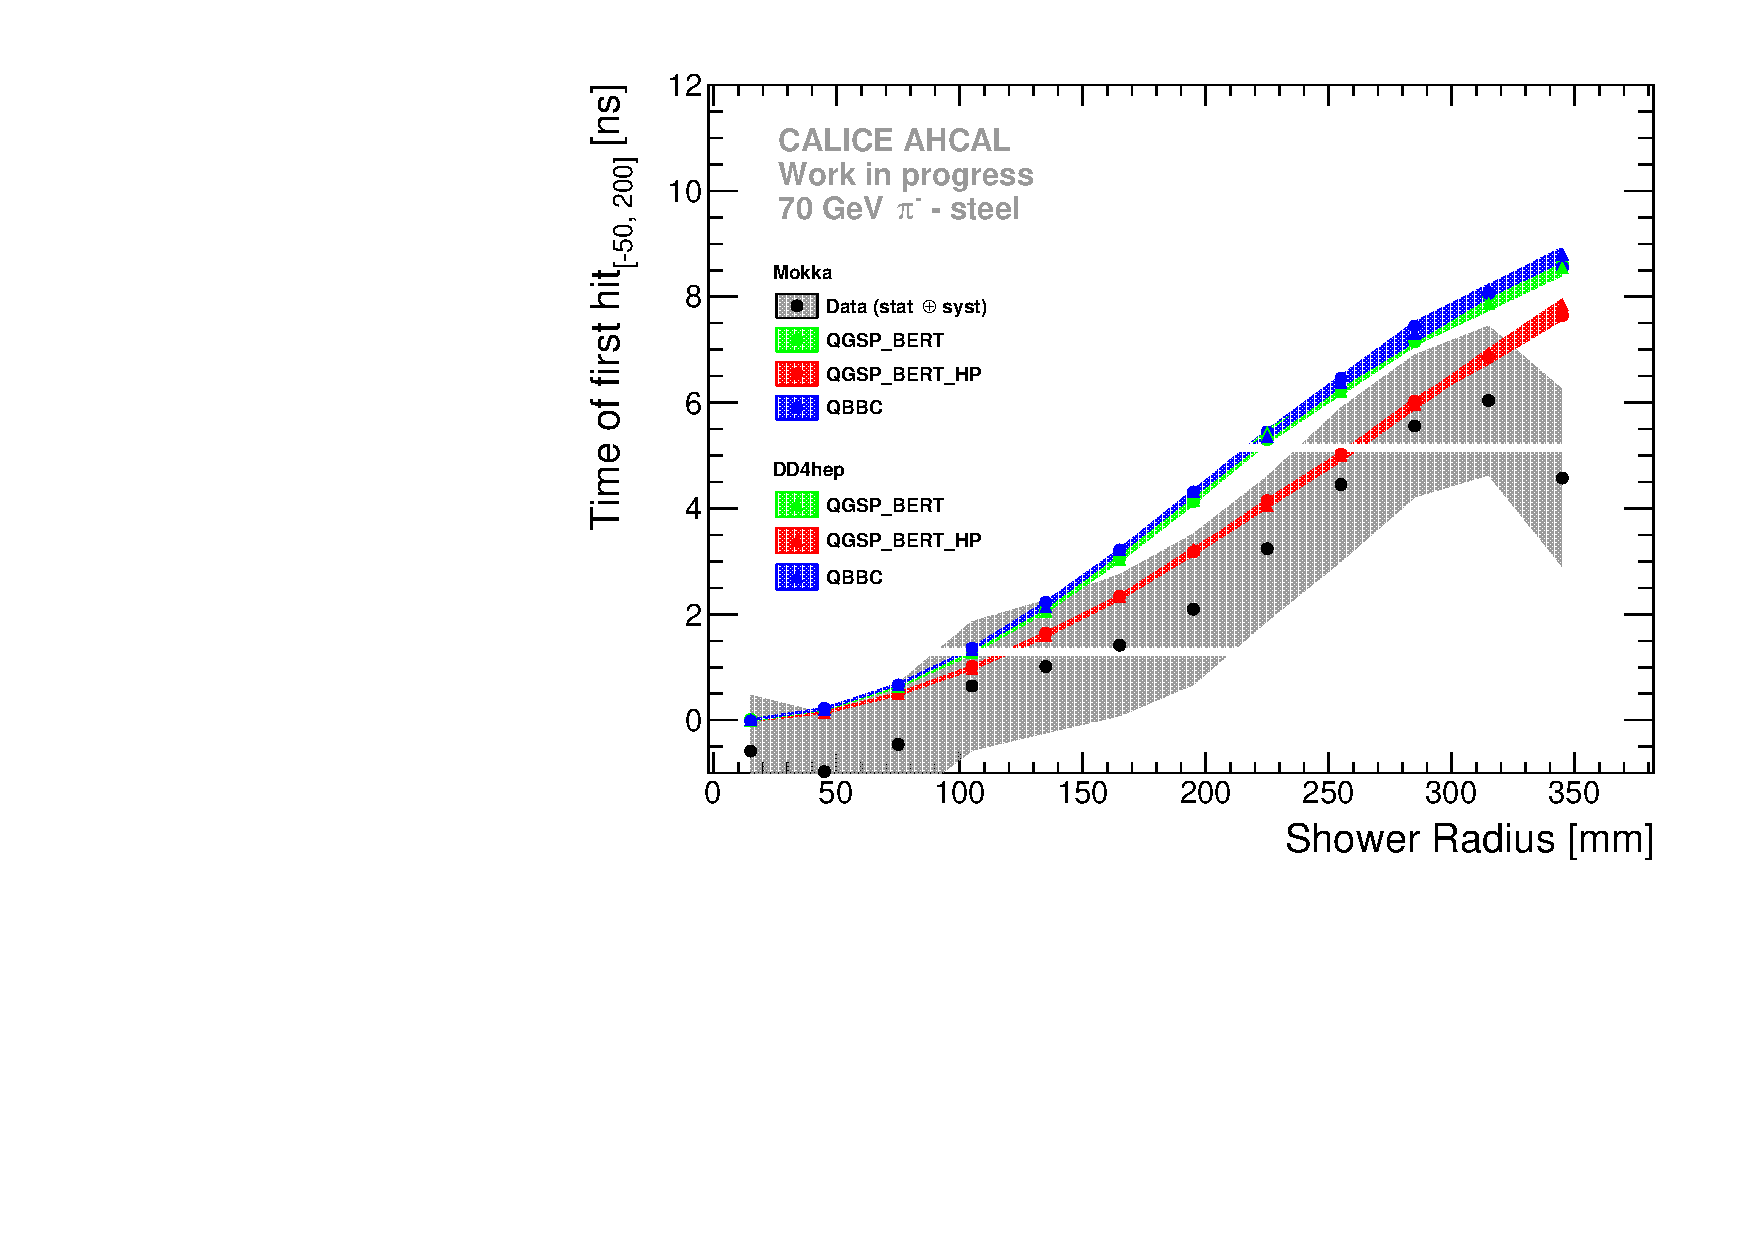
\includegraphics[width=1\textwidth]{../Thesis_Plots/Timing/Pions/Plots/ComparisonToSim/Time_Radius_70GeV_BL.pdf}
		\caption{70 GeV (BL).} \label{fig:Radius_BL_SimData_70GeV}
	\end{subfigure}
	\hfill
	\begin{subfigure}[t]{0.5\textwidth}
		\centering
		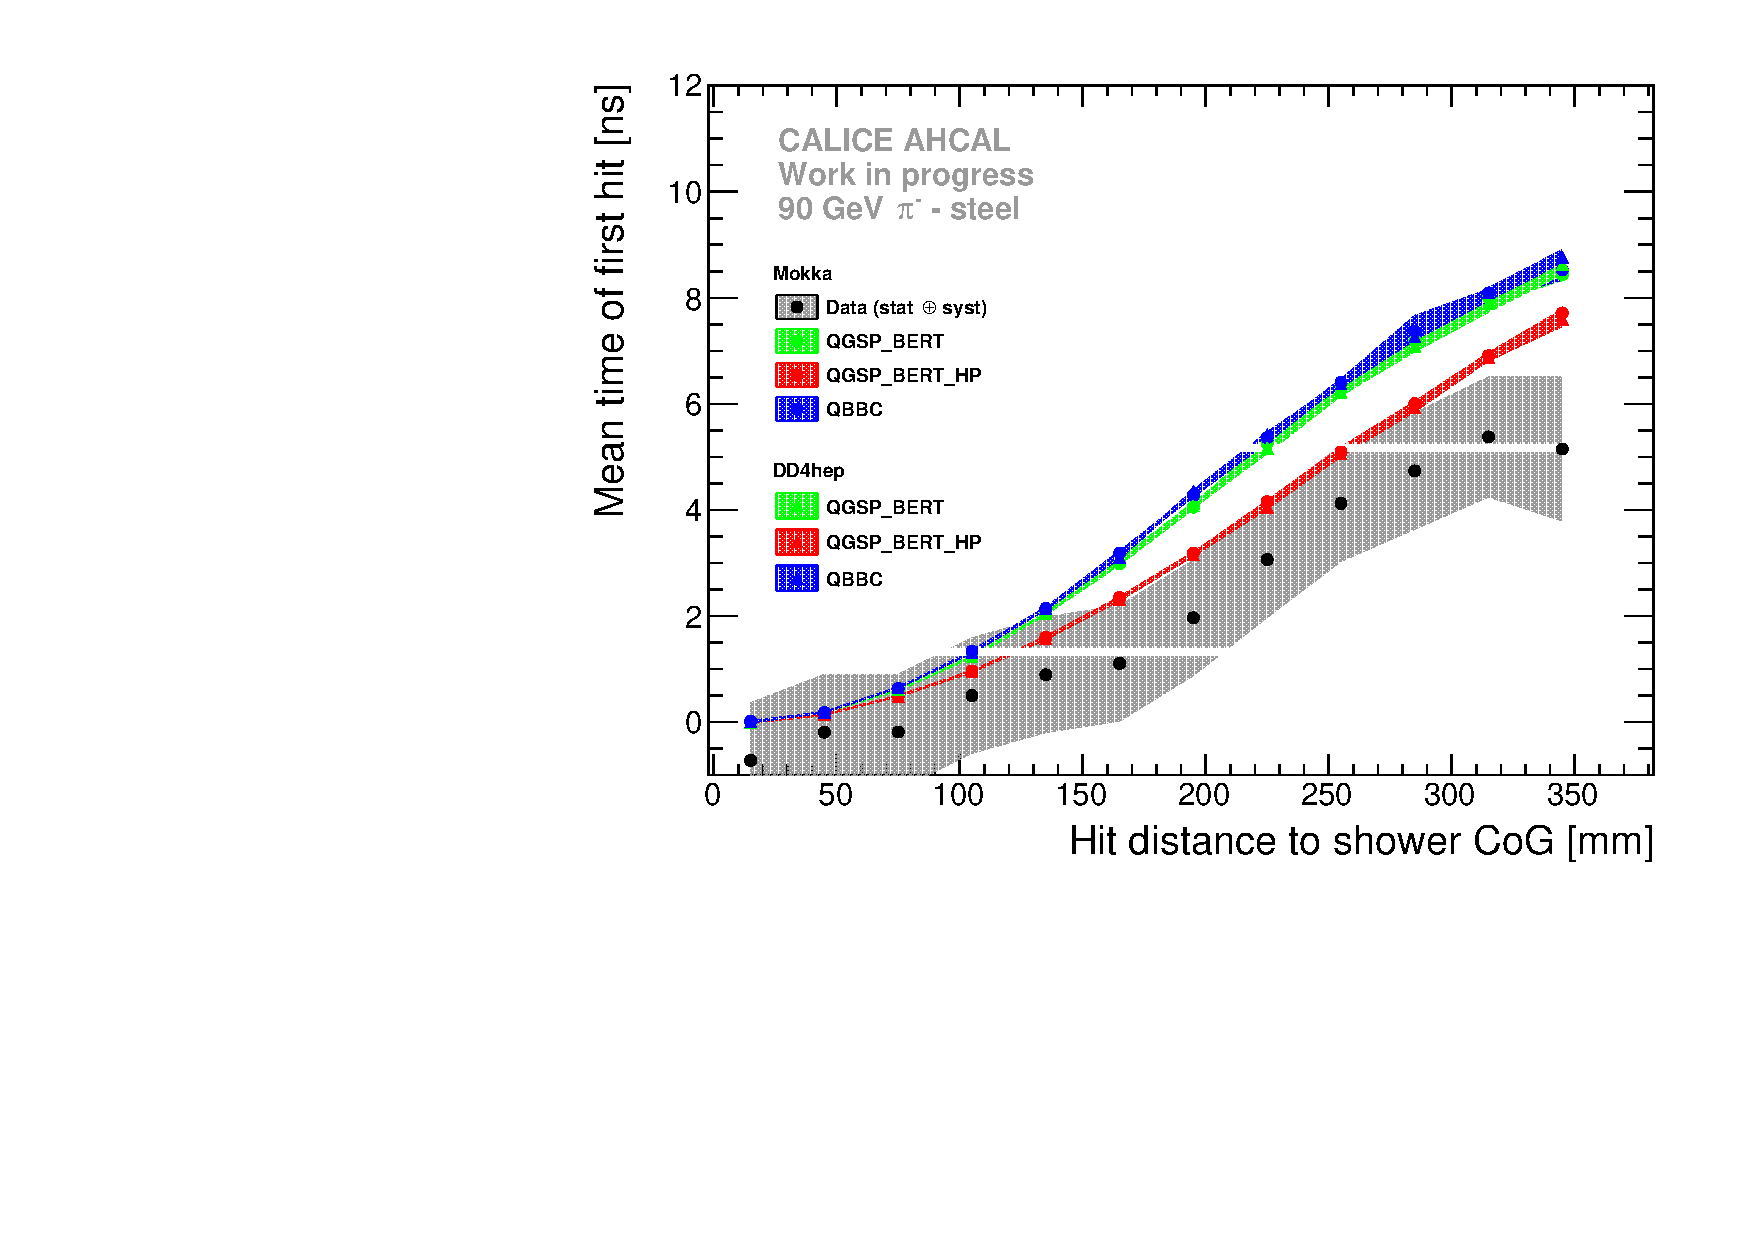
\includegraphics[width=1\textwidth]{../Thesis_Plots/Timing/Pions/Plots/ComparisonToSim/Time_Radius_90GeV_BL.pdf}
		\caption{90 GeV (BL).} \label{fig:Radius_BL_SimData_90GeV}
	\end{subfigure}
	\caption{Comparison between simulations and data of the time of first hit as function of the distance to the shower axis for pion beams between 10 GeV and 90 GeV for the big layers (layers 11 to 14). The grey and color bands shows the systematics.}
	\label{fig:Radius_BL_SimData_Comparison}
\end{figure}

\section{Longitudinal dependence of timing profiles}

The longitudinal dependence of hit time was also looked at. It is expected that the further you are in the calorimeter that more low energy neutrons contribute to the energy deposition thus enhancing the late tail. The figure \ref{fig:Depth_Comparison} shown the mean time of first hit as function of the layer position for muon, electron and pion beams.

\begin{figure}[htbp!]
	\begin{subfigure}[t]{0.5\textwidth}
		\centering
		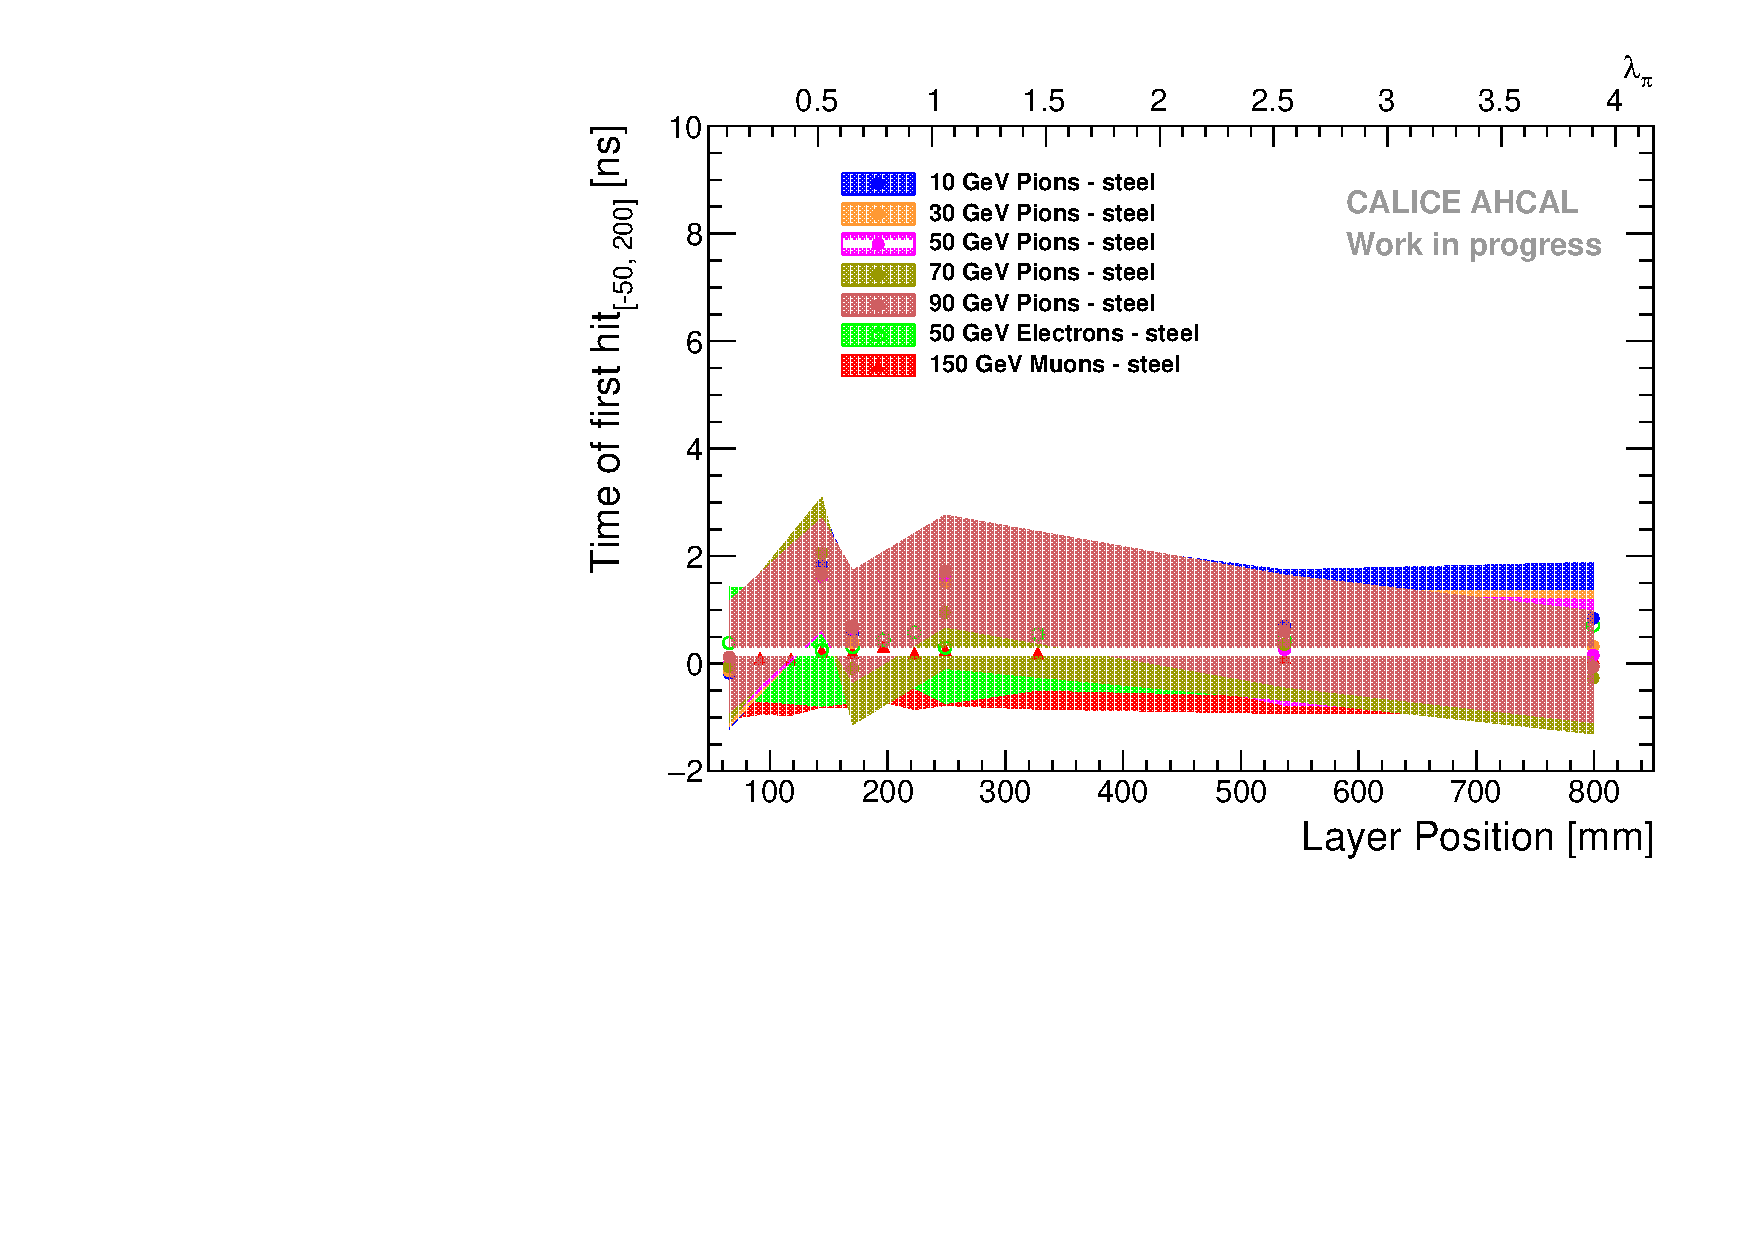
\includegraphics[width=1\textwidth]{../Thesis_Plots/Timing/Pions/Plots/Timing_Depth_Comparison_ShortAsymRange.pdf}
		\caption{Time of first hit as function of the layer position.} \label{fig:Depth_Comparison}
	\end{subfigure}
	\hfill
	\begin{subfigure}[t]{0.5\textwidth}
		\centering
		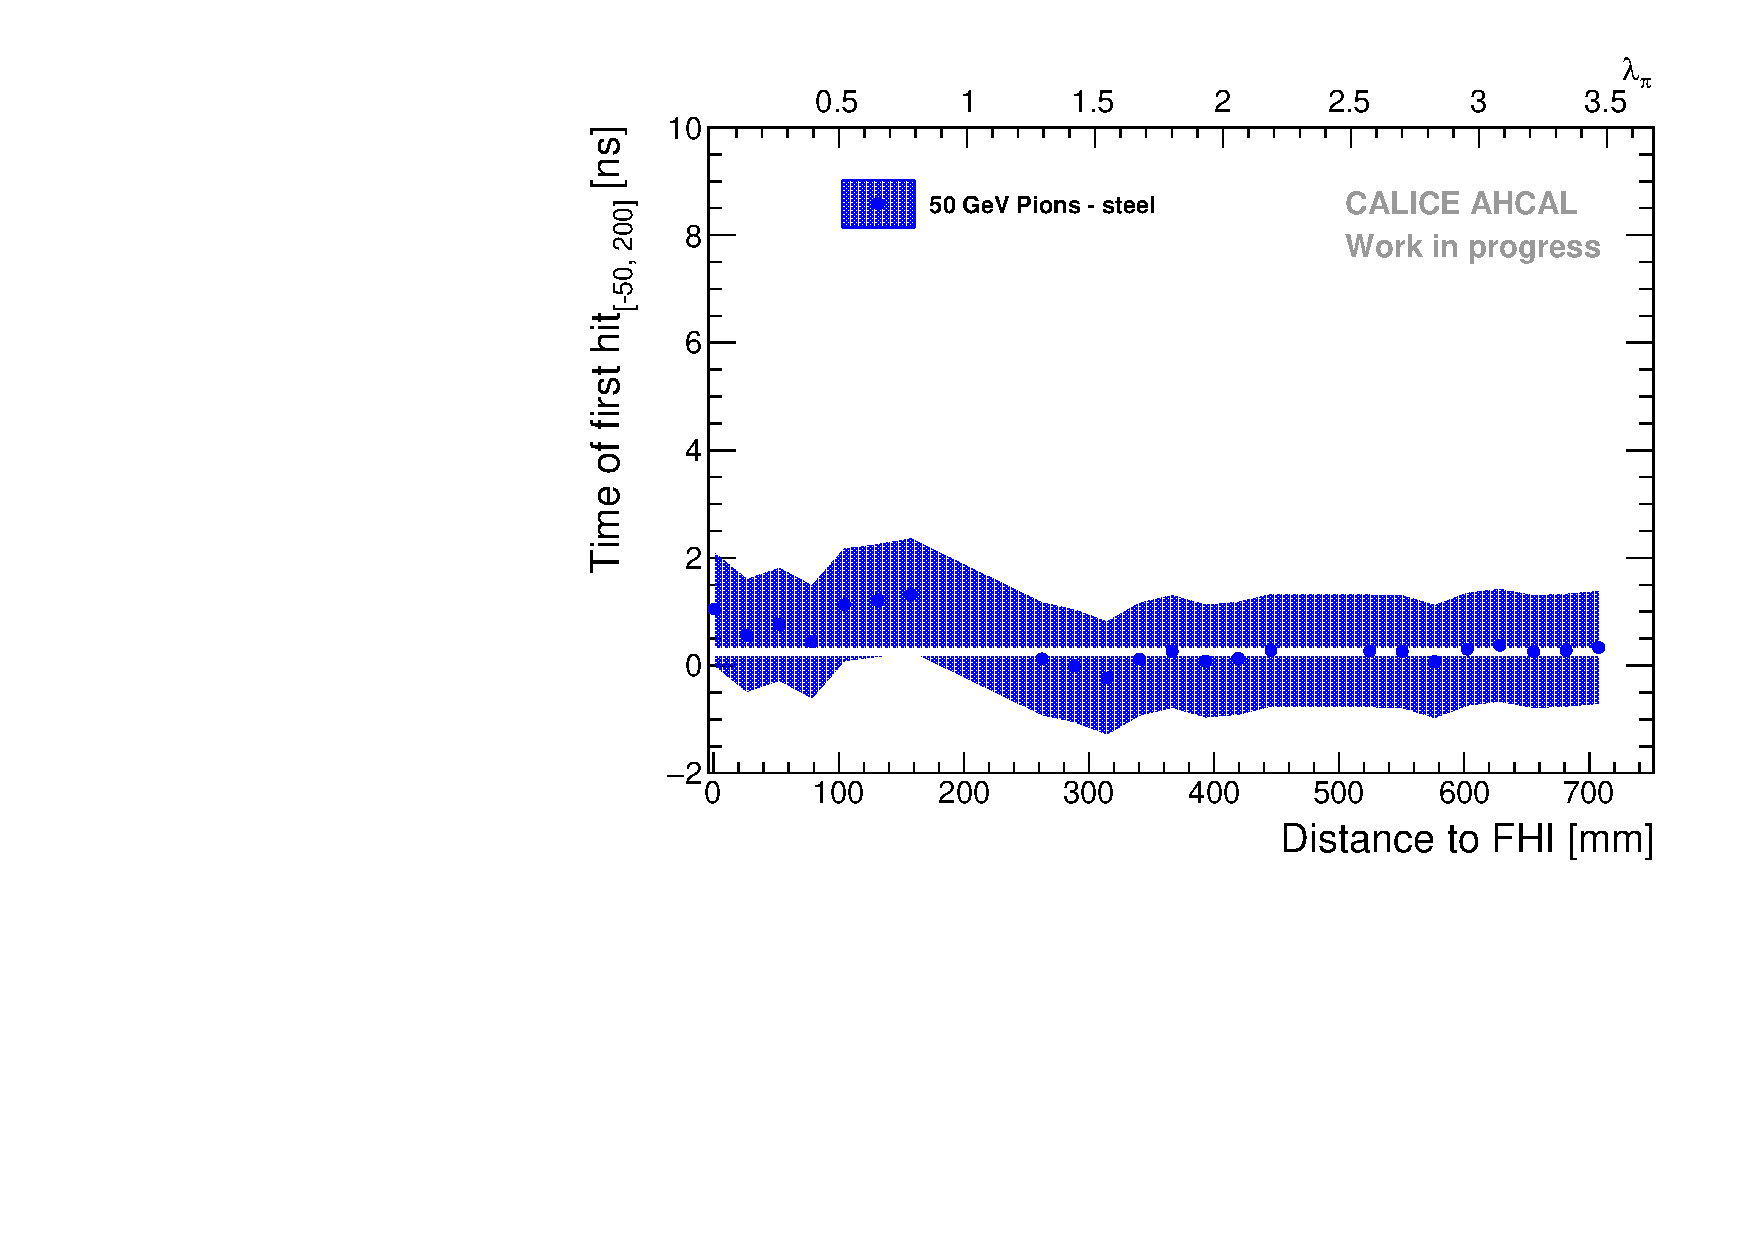
\includegraphics[width=1\textwidth]{../Thesis_Plots/Timing/Pions/Plots/Timing_Depth_Comparison_ShortAsymRange_ShowerStart.pdf}
		\caption{Time of first hit as function of the distance to the FHI.}\label{fig:Depth_Comparison_FHI}
	\end{subfigure}
	\caption{The left plot shows that all distributions are compatible with a flat distribution for the time of first hit as function of the layer position. The right plot shows the same as function of the distance to the reconstructed FHI.}
	\label{fig:DepthProfile}
\end{figure}

It seems that the observation in the data is compatible with no increase of the time with the layer depth within systematics. This may be due to the fact that the sensitivity to this late component is suppressed by the time resolution of the calorimeter as well as the systematic errors. An attempt to get a better sensitivity was to look at the mean time of first hit as function of the depth from the reconstructed FHI as shown in figure \ref{fig:Depth_Comparison_FHI}. The same conclusion within systematics that it is compatible with a flat distribution around $t=0$.

\begin{figure}[htbp!]
	\centering
	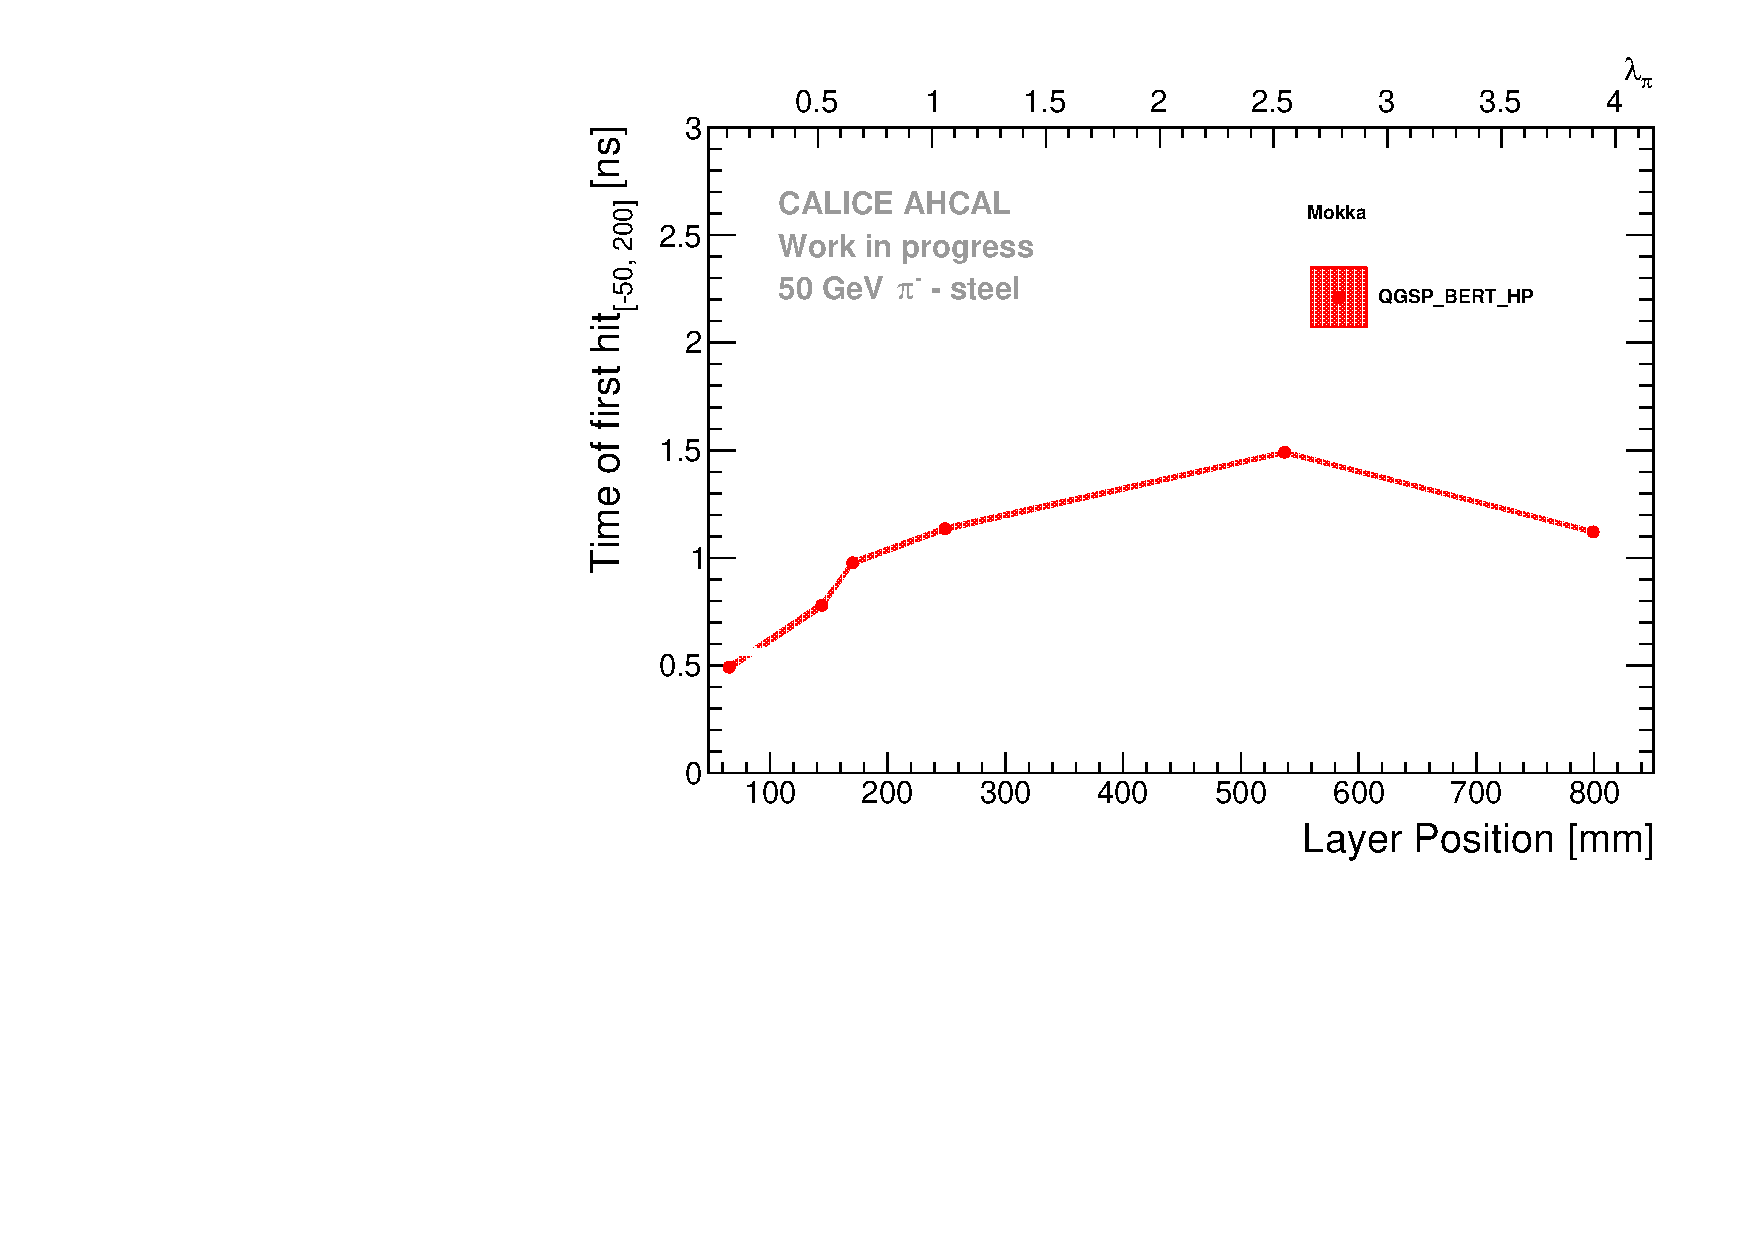
\includegraphics[width=0.6\textwidth]{../Thesis_Plots/Timing/Pions/Plots/Time_Depth_50GeV_QGSP_BERT_HP_noSmearing.pdf}
	\caption{Time of first hit as function of the layer position for 50 GeV pions in simulation with the QGSP\_BERT\_HP physics list with no time smearing. The bands represent the systematic uncertainty.}
	\label{fig:Depth_Sim_noSmearing}
\end{figure}

The longitudinal timing profile was also compared to simulations. As in the data, the mean time of first hit is compatible with a flat distribution around $t=0$. All simulations agree with the data within systematics. The timing resolution of the AHCAL may be too high in order to be sensitive to any small changes of the mean time over the calorimeter depth. The simulation without time smearing was looked at as shown in figure \ref{fig:Depth_Sim_noSmearing}. It shows that there is an increase of the mean time of first hit as function of the layer in the order of 1 ns and confirms that due to the electronics time resolution this is not visible in data.

\begin{figure}[htbp!]
	\begin{subfigure}[t]{0.5\textwidth}
		\centering
		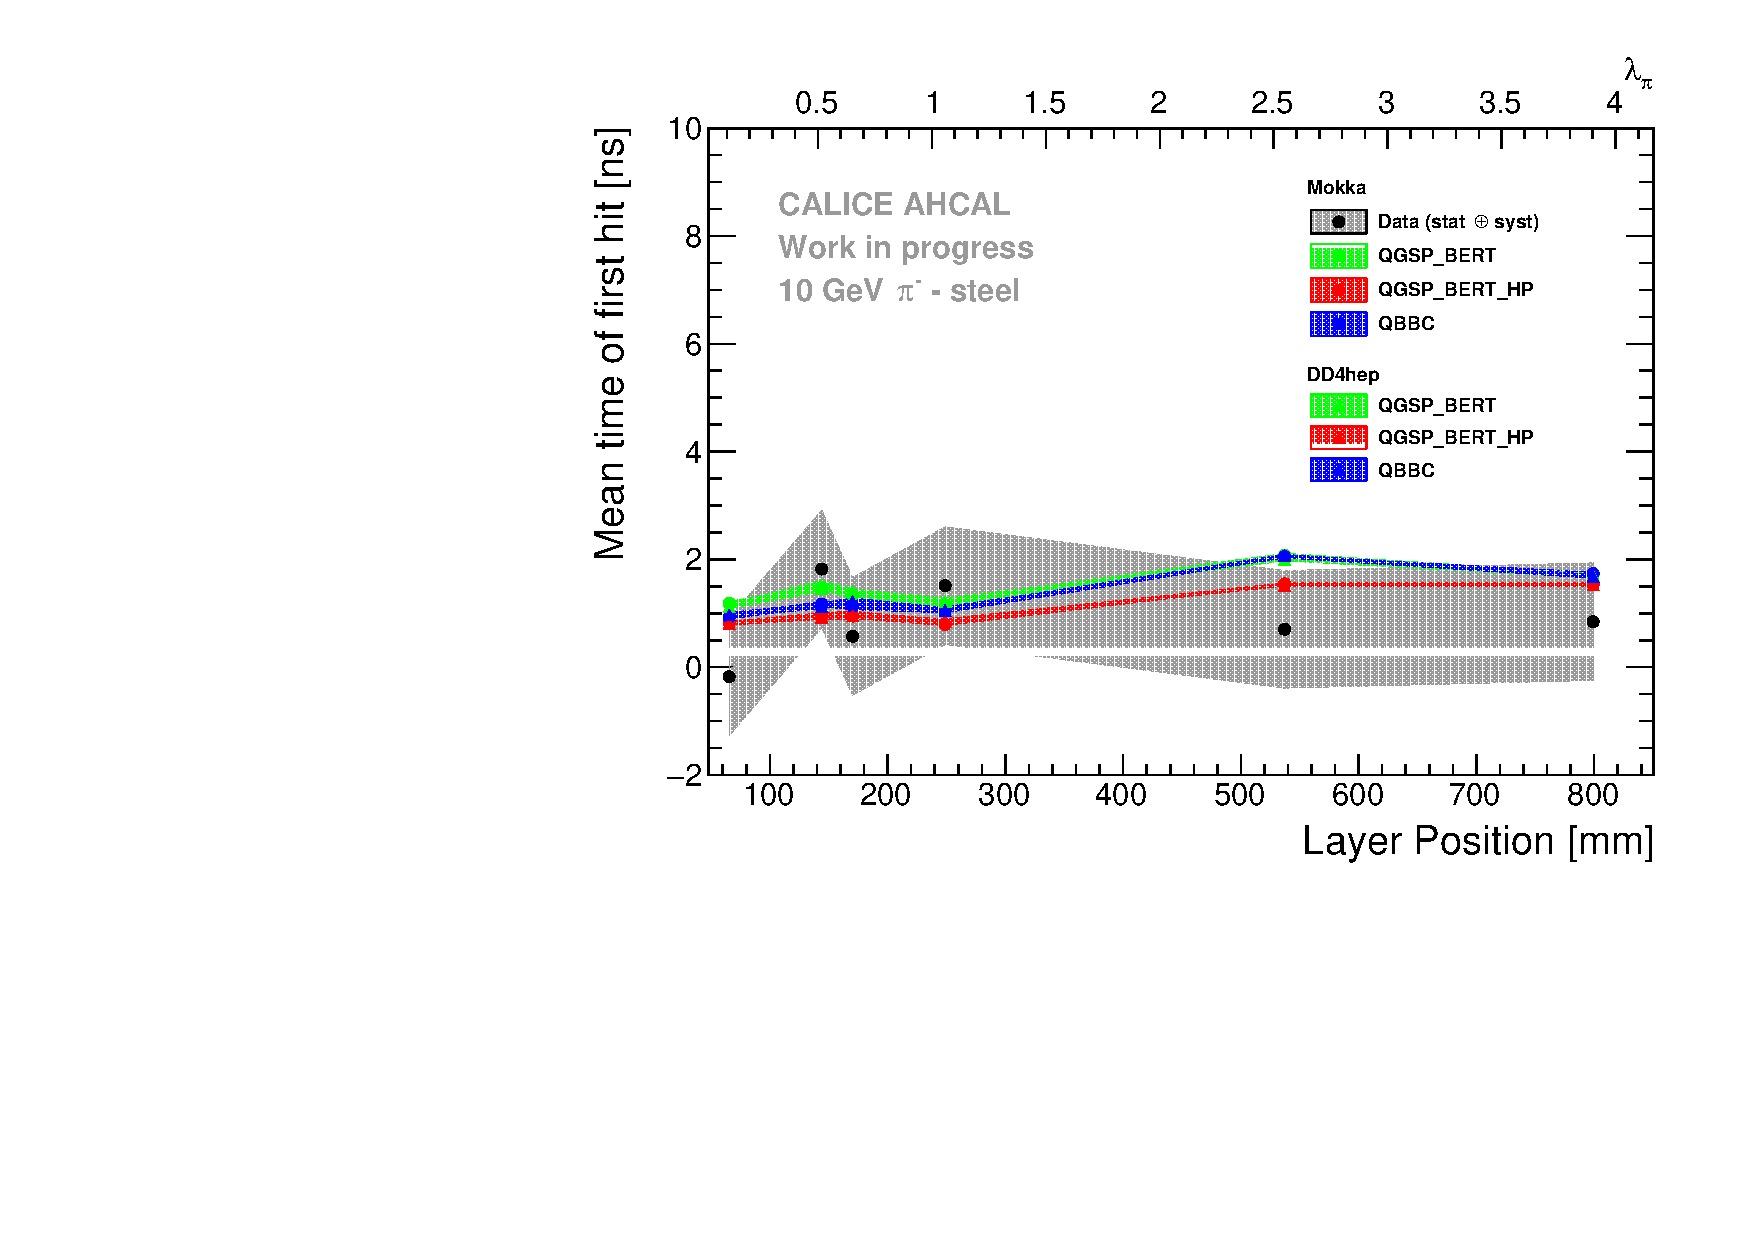
\includegraphics[width=1\textwidth]{../Thesis_Plots/Timing/Pions/Plots/ComparisonToSim/Time_Depth_10GeV.pdf}
		\caption{10 GeV.}\label{fig:Depth_SimData_10GeV}
	\end{subfigure}
	\hfill
	\begin{subfigure}[t]{0.5\textwidth}
		\centering
		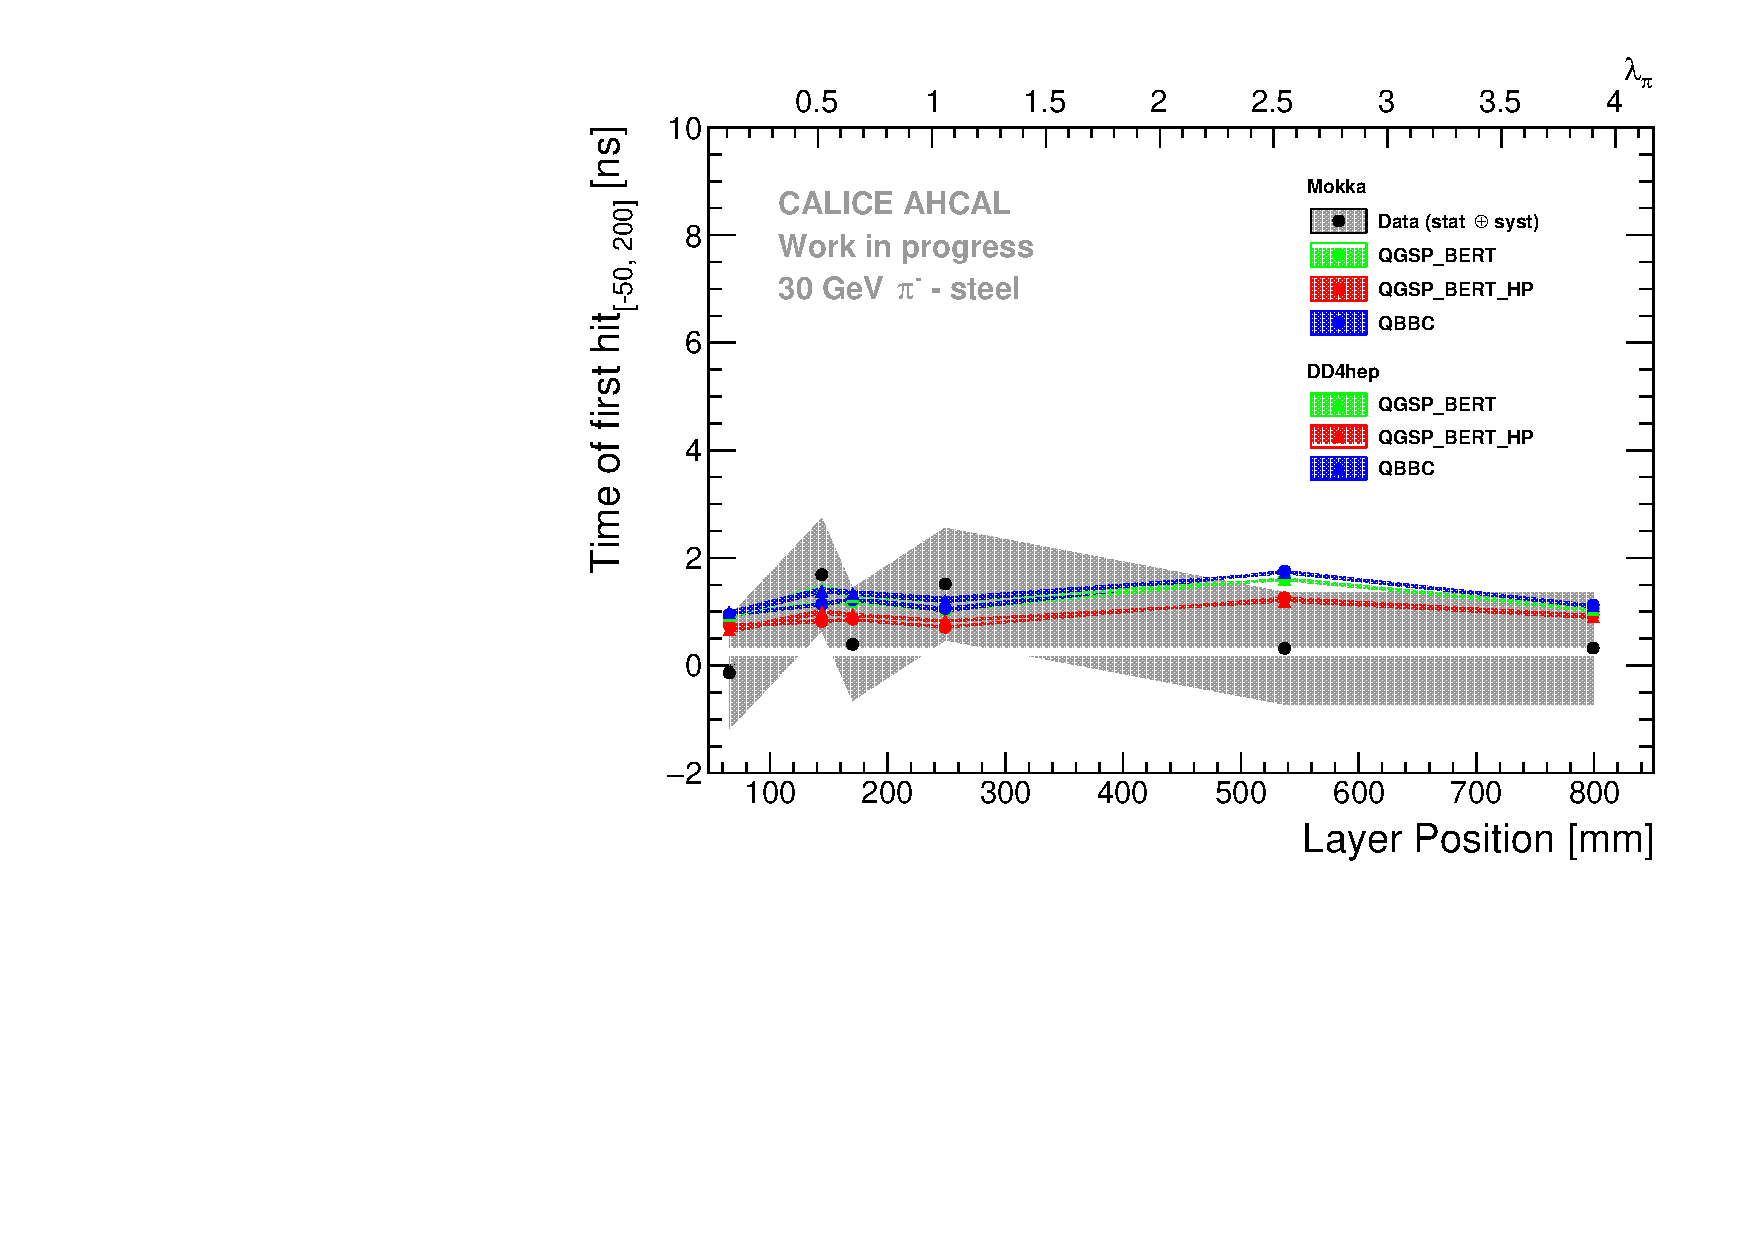
\includegraphics[width=1\textwidth]{../Thesis_Plots/Timing/Pions/Plots/ComparisonToSim/Time_Depth_30GeV.pdf}
		\caption{30 GeV.} \label{fig:Depth_SimData_30GeV}
	\end{subfigure}
	\hfill
	\begin{subfigure}[t]{0.5\textwidth}
		\centering
		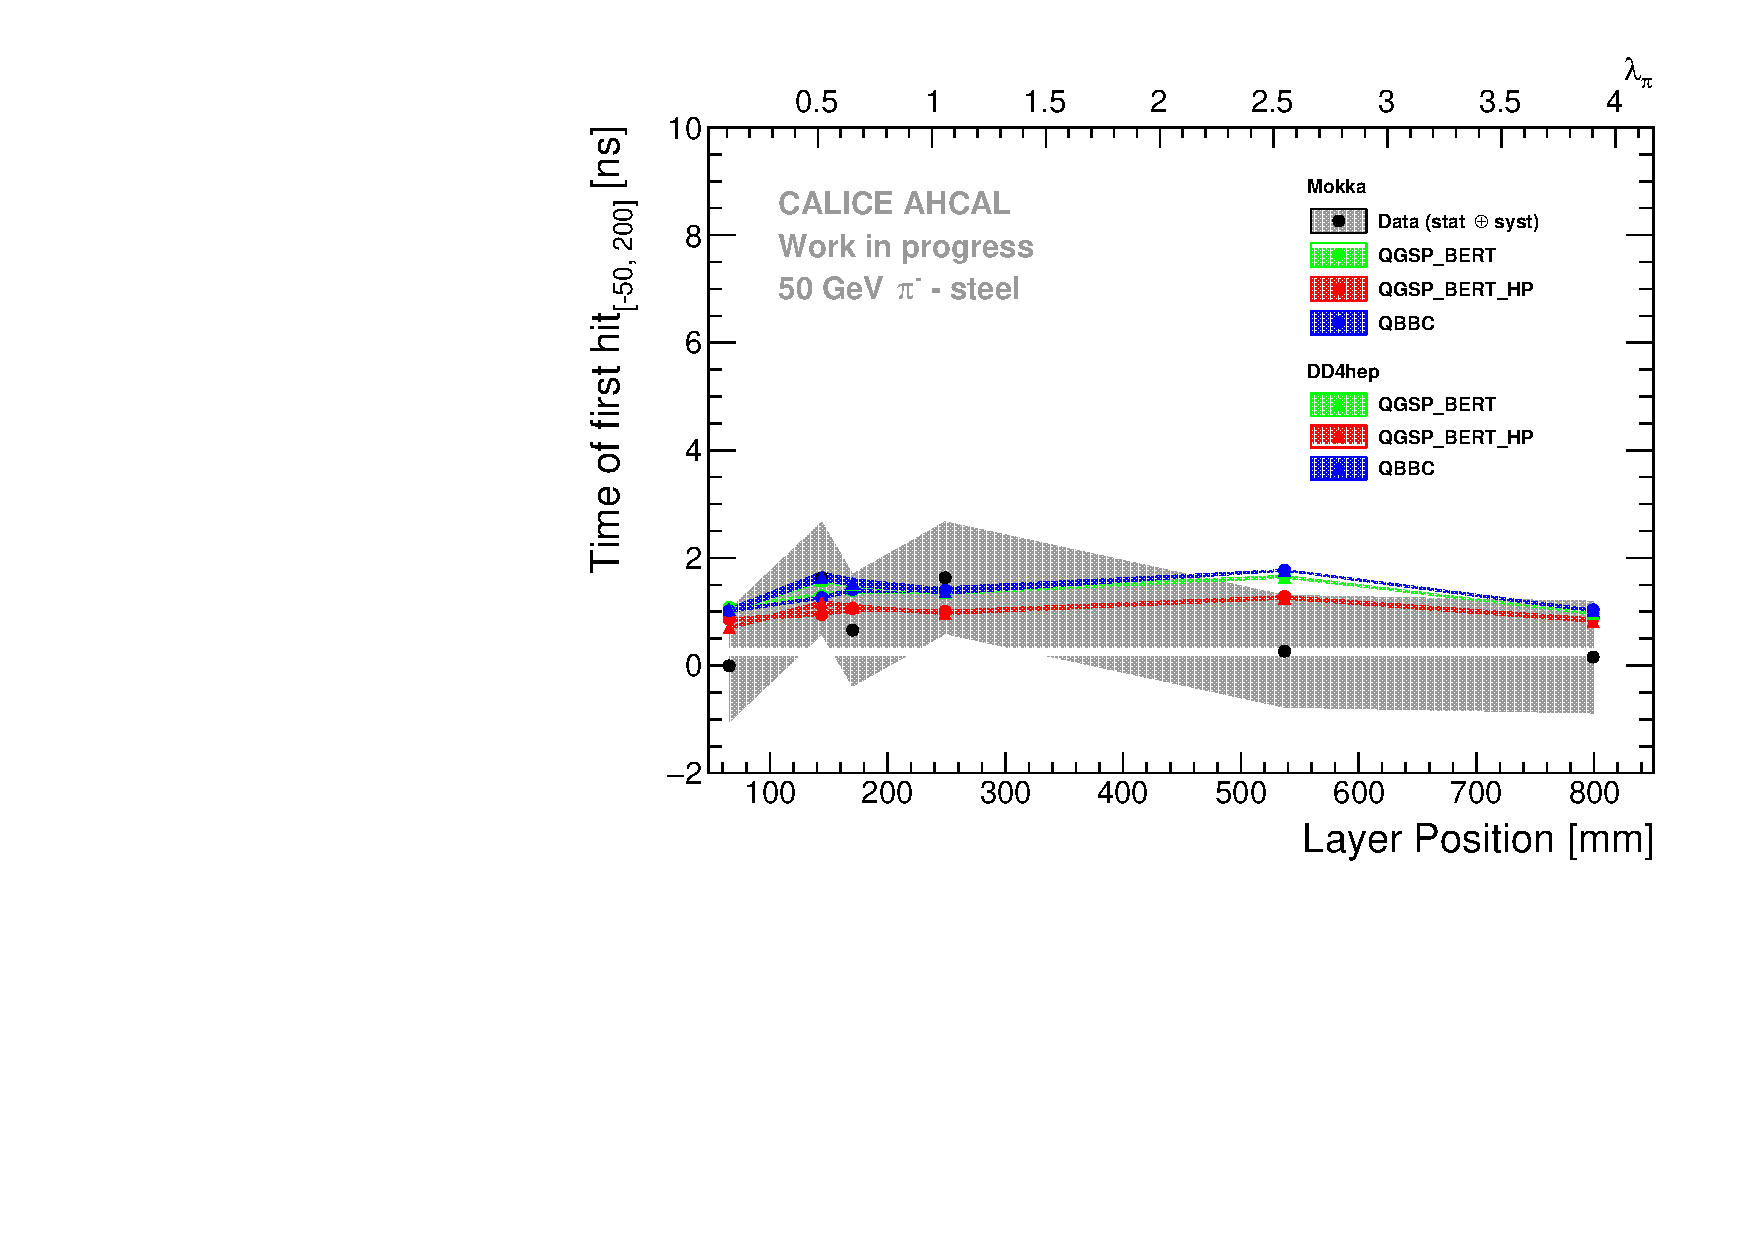
\includegraphics[width=1\textwidth]{../Thesis_Plots/Timing/Pions/Plots/ComparisonToSim/Time_Depth_50GeV.pdf}
		\caption{50 GeV.} \label{fig:Depth_SimData_50GeV}
	\end{subfigure}
	\hfill
	\begin{subfigure}[t]{0.5\textwidth}
		\centering
		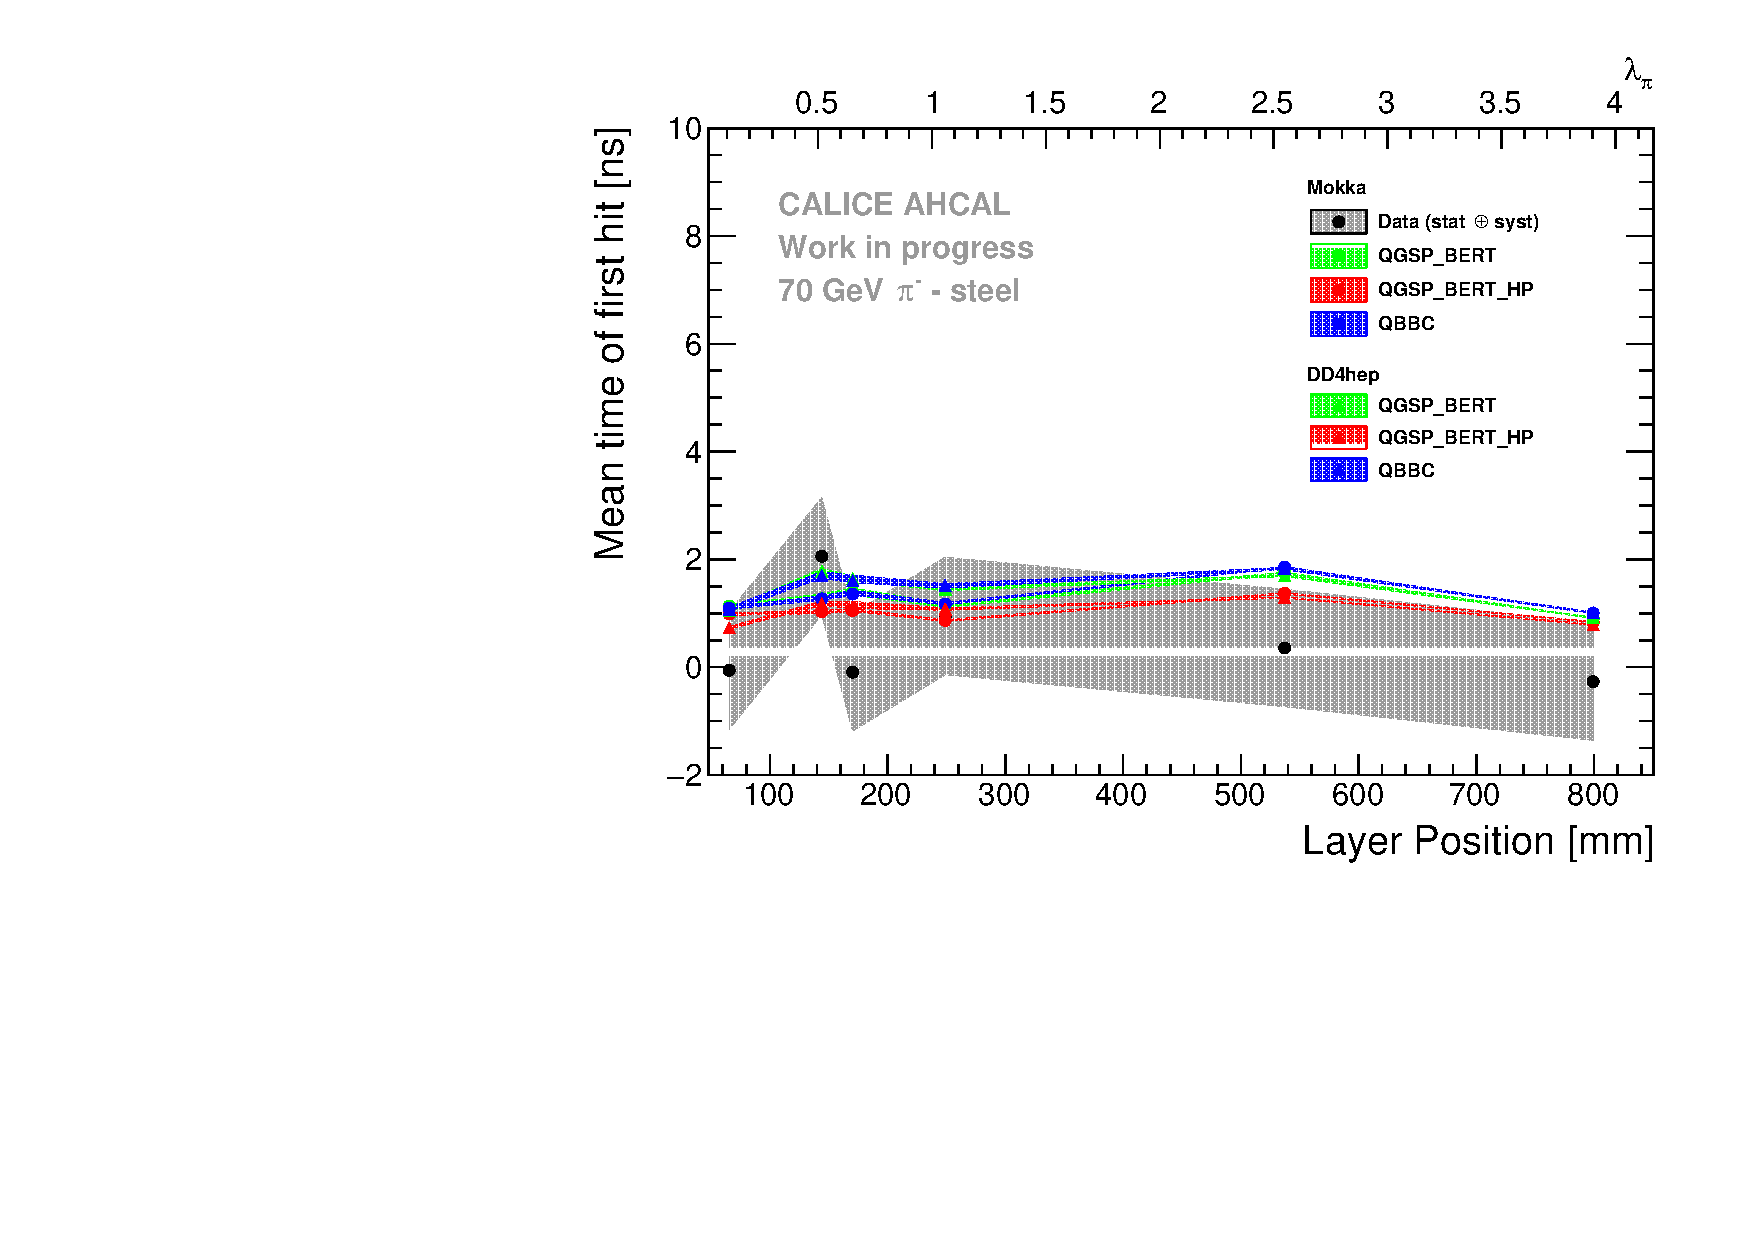
\includegraphics[width=1\textwidth]{../Thesis_Plots/Timing/Pions/Plots/ComparisonToSim/Time_Depth_70GeV.pdf}
		\caption{70 GeV.} \label{fig:Depth_SimData_70GeV}
	\end{subfigure}
	\hfill
	\begin{subfigure}[t]{0.5\textwidth}
		\centering
		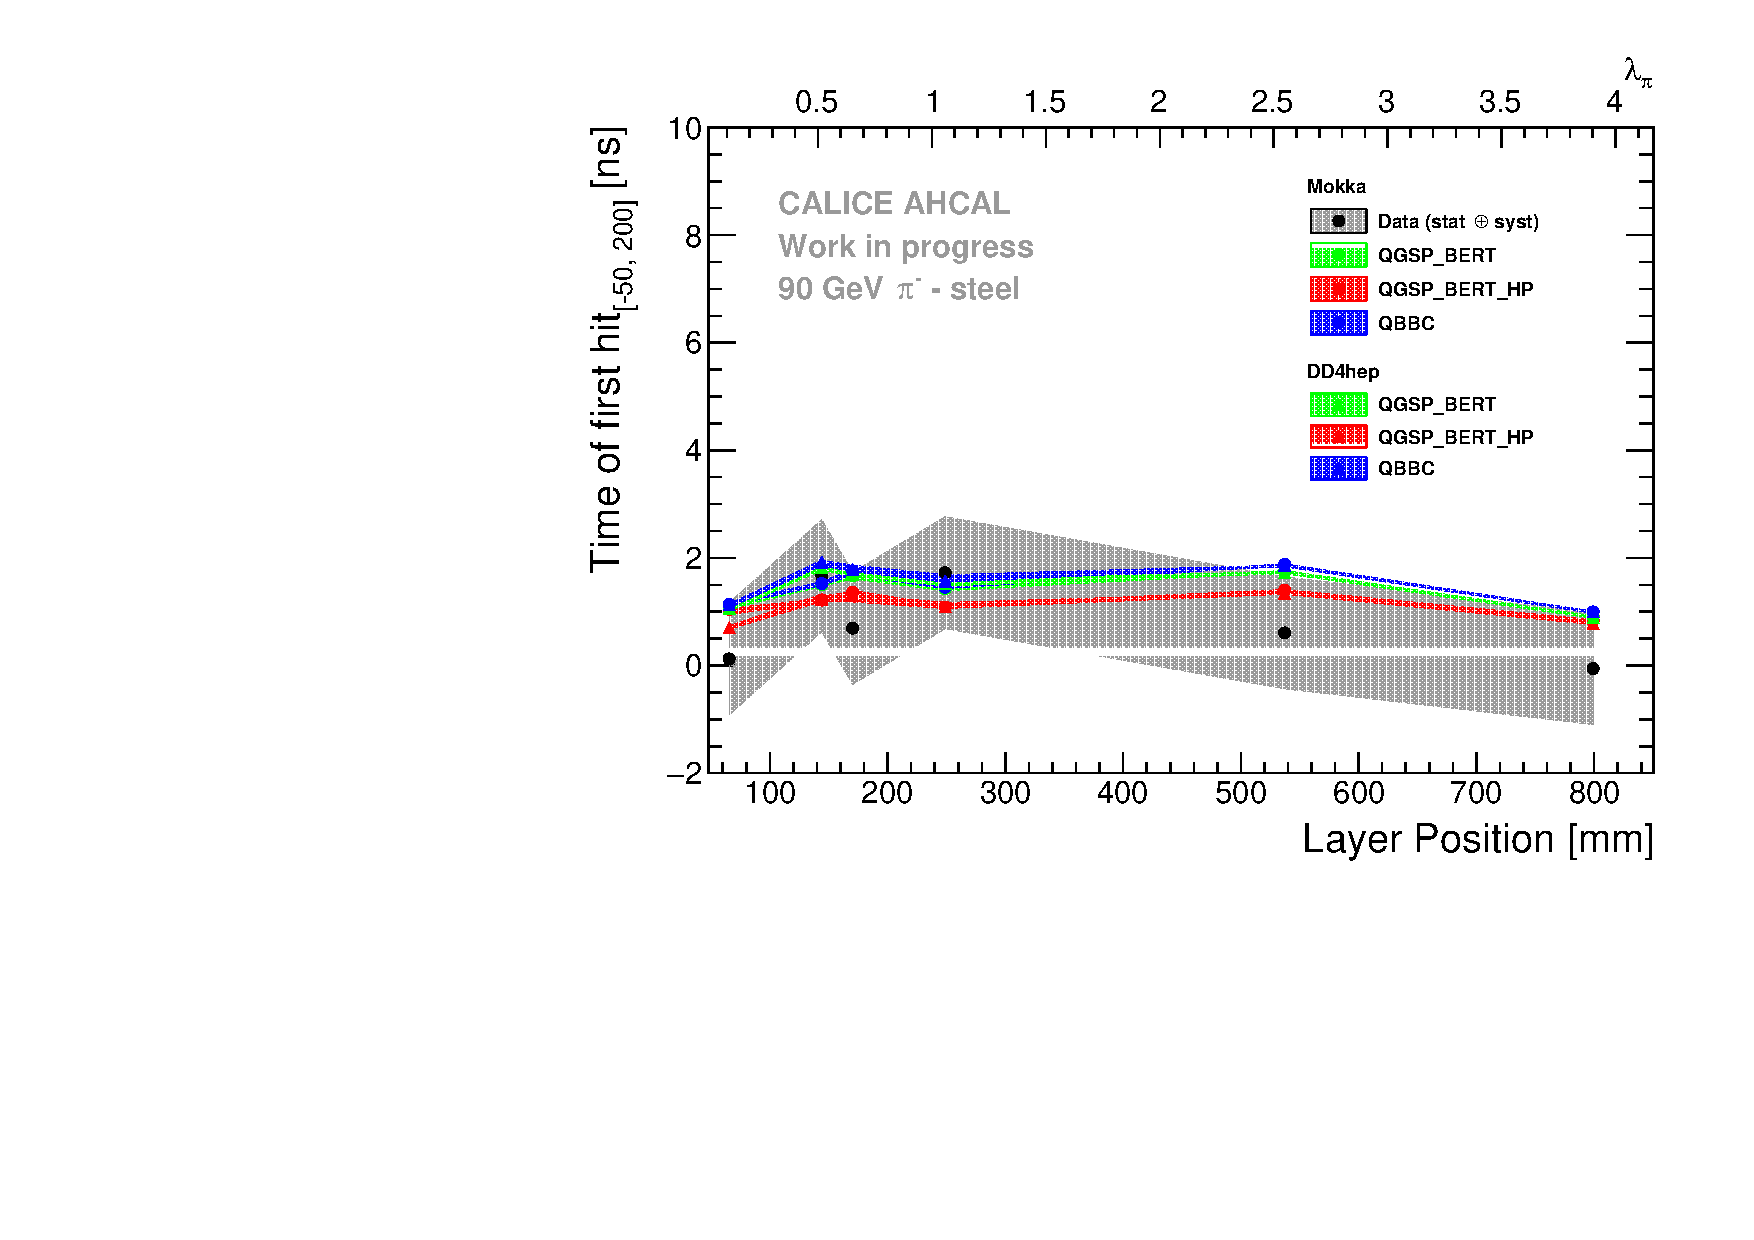
\includegraphics[width=1\textwidth]{../Thesis_Plots/Timing/Pions/Plots/ComparisonToSim/Time_Depth_90GeV.pdf}
		\caption{90 GeV.} \label{fig:Depth_SimData_90GeV}
	\end{subfigure}
	\caption{Comparison between simulations and data of the time of first hit as function of the layer position for pion beams between 10 GeV and 90 GeV. The grey and color bands shows the systematics.}
	\label{fig:Depth_SimData_Comparison}
\end{figure}

\section{Time correlations between layers}

The advantage of this studied prototype over T3B is the possibility to investigate the possible time correlations between layers. This has been looked at as shown in figures \ref{fig:Time_Corr_short} and \ref{fig:Time_Corr_long} for the 50 GeV pion sample. For this, the data below 50 ns is ignored as only the tail of the timing distributions is interesting. Two types of correlations were investigated, short and long. The procedure is done by looking at each hit in layer $i$ and checking in layer $i+1$ for a hit within a distance of 60 mm in the $x:y$ plane. If a hit is found, both times are plotted against each other. If more than one hit is found in layer $i+1$ within a distance of 60 mm, the closest in the $x:y$ plane is taken. For the short correlation, the layers 6 and 7 were chosen, corresponding to 1 $X_0$ or 0.1 $\lambda_{\pi}$. As for the long, the layers 13 and 14 were selected, corresponding to 10 $X_0$ or 1 $\lambda_{\pi}$. These were chosen due to the fact that few layers were working properly. It is expected that EM sub-showers can lead to a correlation of hit times for layers 6 and 7, while for layer 13 and 14 as they are too far apart and therefore would not show much less correlation.

\begin{figure}[htbp!]
	\begin{subfigure}[t]{0.5\textwidth}
		\centering
		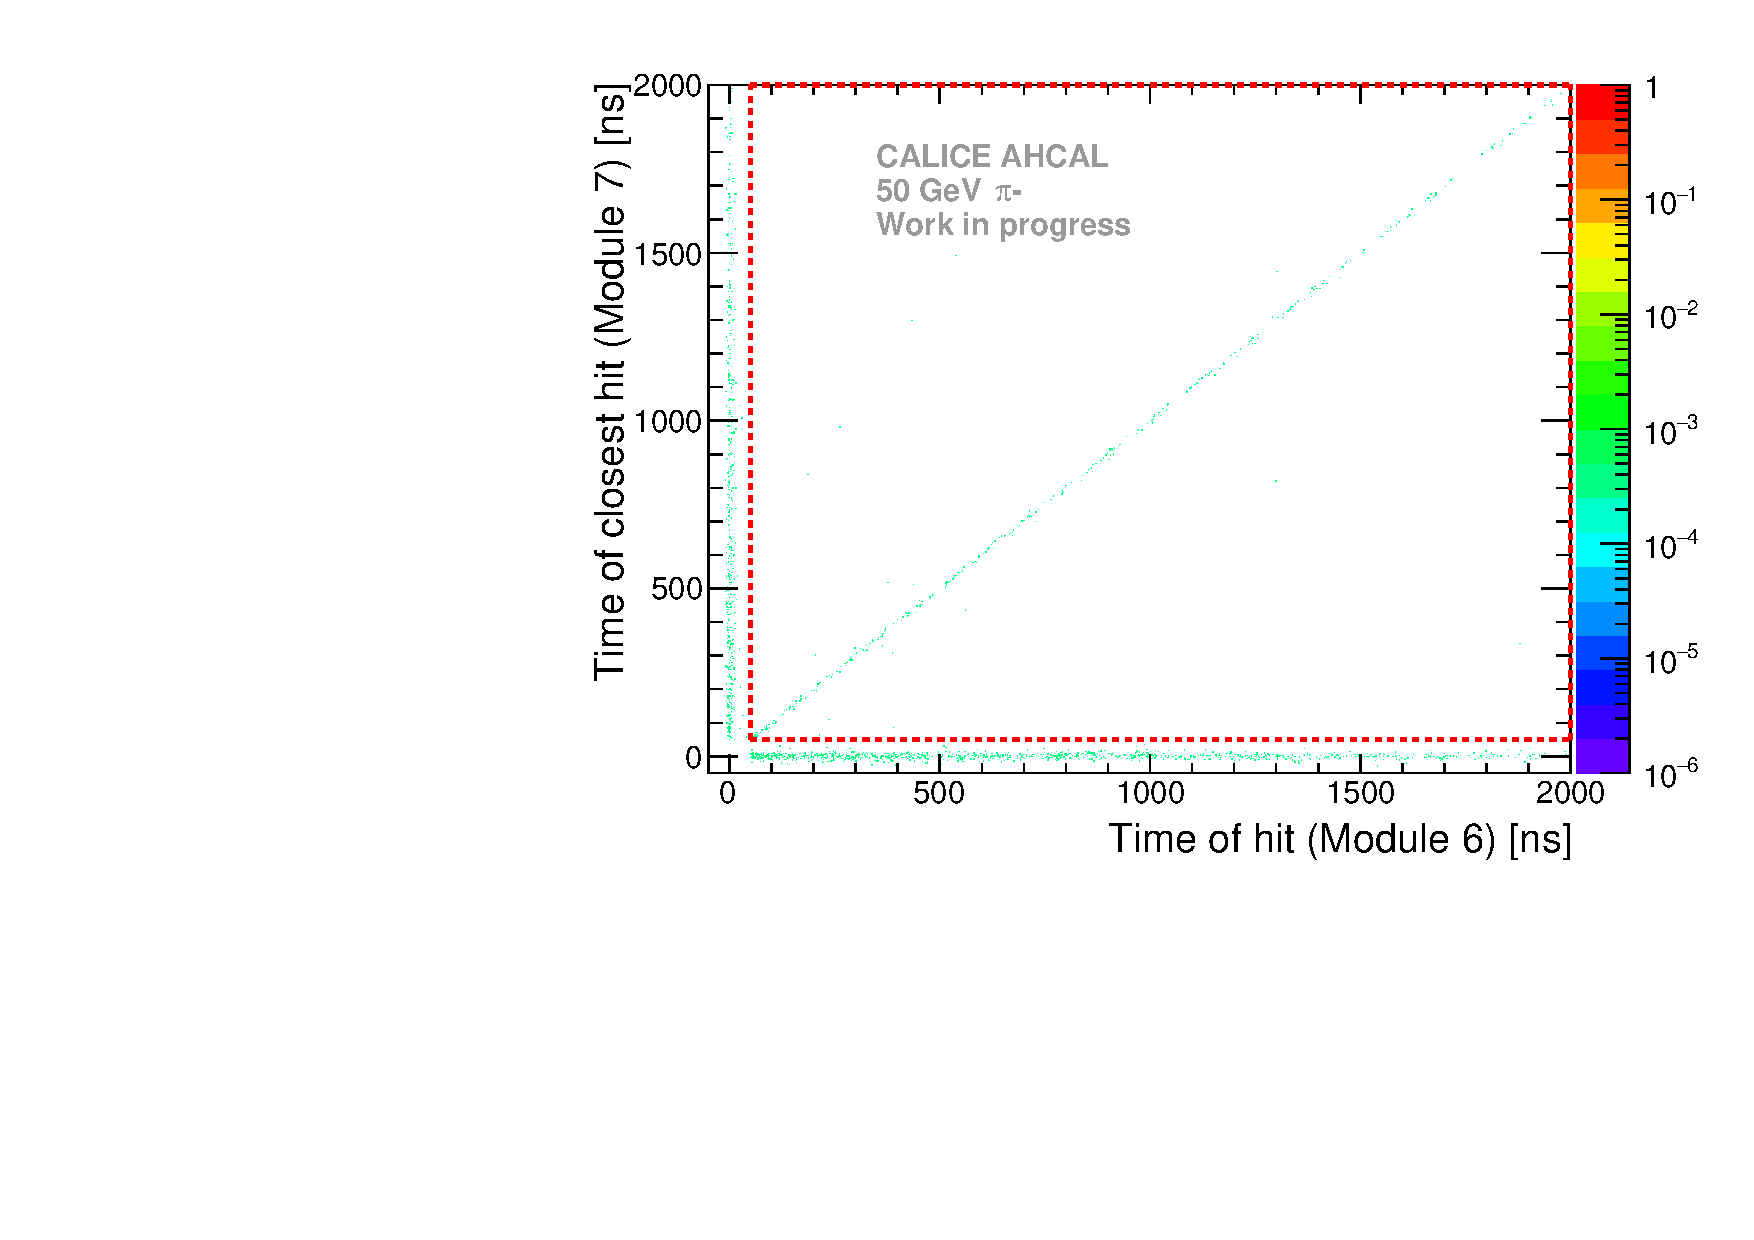
\includegraphics[width=1\textwidth]{../Thesis_Plots/Timing/Pions/Plots/Time_Correlation_short.pdf}
		\caption{Time correlation between layer 6 and 7 for 50 GeV pions.} \label{fig:Time_Corr_short}
	\end{subfigure}
	\hfill
	\begin{subfigure}[t]{0.5\textwidth}
		\centering
		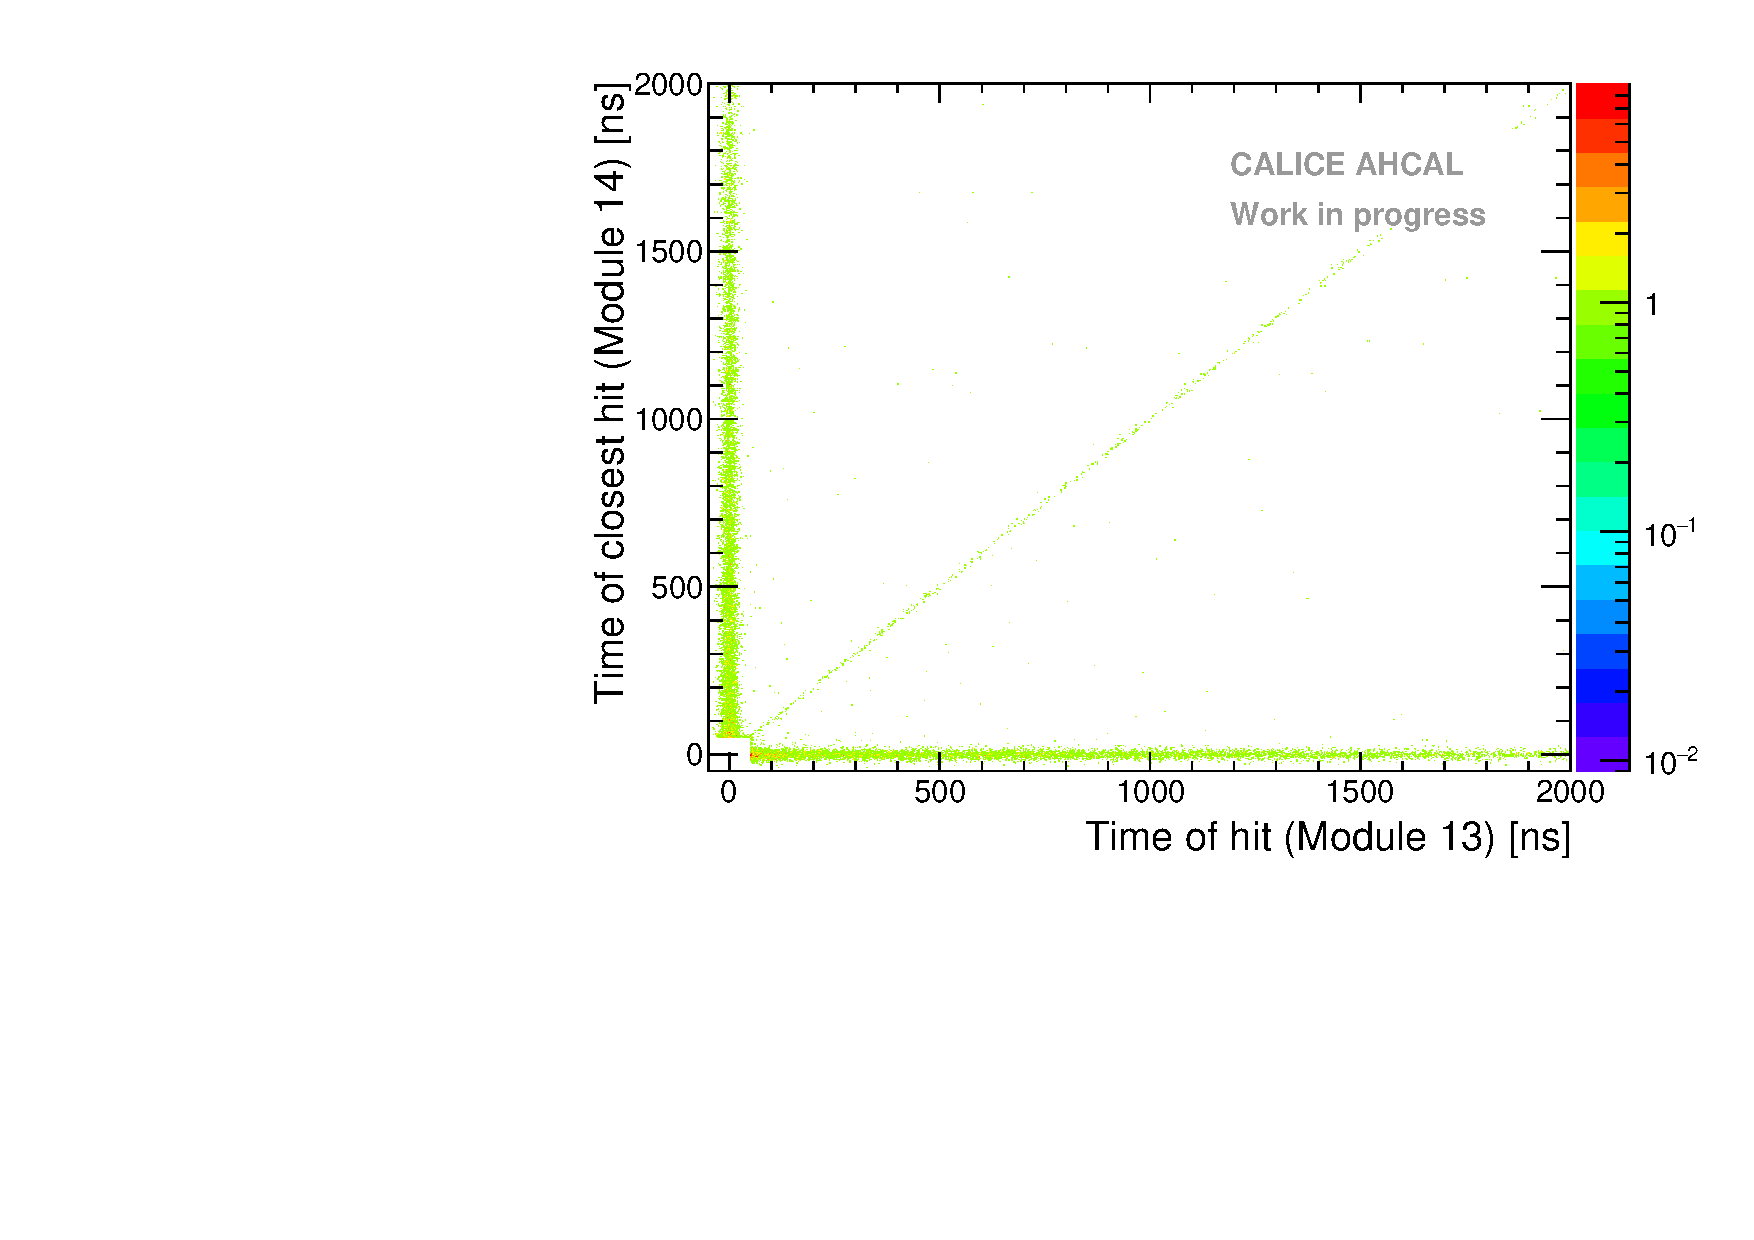
\includegraphics[width=1\textwidth]{../Thesis_Plots/Timing/Pions/Plots/Time_Correlation_long.pdf}
		\caption{Time correlation between layer 13 and 14 for 50 GeV pions.}\label{fig:Time_Corr_long}
	\end{subfigure}
	\caption{The left plot shows the time correlation between layer 6 and 7 separated by 1 $X_0$. The right plot shows the time correlation for layers 13 and 14 separated by 1 $\lambda_{\pi}$. Each bins are normalized to the number of entries in the 2D histogram. Both plots show a visible time correlation.}
	\label{fig:TimeCorrelation}
\end{figure}

The figures show that a correlation is visible in both cases in the data. To quantify this, the ratio $R$ of the number of hits per time bin between 50 ns and \SI{2}{\micro\second} and the total number of entries per bin $N_{tot}$ defined by the red box in each plots is calculated:

\begin{equation}
	R = \frac{\int_{50 ns}^{2 \mu s} \int_{50 ns}^{2 \mu s} \frac{dN_i(t)}{dt_i} \frac{dN_j(t)}{dt_j} dt_i dt_j}{N_{tot}}
\end{equation}

The results show that 18.14\% of the entries are in the $R$ region for the short correlation. This could be indeed possible due to the proximity of the layer and may come from EM sub-showers in the hadron shower. For the long correlation, 3.24\% of the entries are in the $R$ region. This represents a substantial amount of hits that are correlated. This is not clear the origin of this correlation but it may come from the fact that the suppression of the multiple particle events that is not suppressed enough and decrease the sensitivity as an example is shown in figure \ref{fig:DoubleParticleEvent}.

\begin{table}[htb!]
	\centering
	\renewcommand*{\arraystretch}{1.3}
	\caption{Table with the integral in \% of events in the $R$ region (red box). The top number is for \mokka simulations, the bottom one is for \ddhep.}
	\label{table:Correlation_DataSim}
	\begin{tabular}{@{} |p{5cm}|cc| @{}}
		\hline
		Type & Short [\%] & Long [\%]\\
		\hline
		\multirow{2}{*}{Data} & \multirow{2}{*}{18.14} & \multirow{2}{*}{3.24}\\ & &\\
		\hline
		\multirow{2}{*}{QGSP\_BERT} & 3.93 & 0.66\\ & 2.30 & 0.50\\
		\hline
		\multirow{2}{*}{QGSP\_BERT\_HP} & 4.01 & 0.72\\ & 2.27 & 0.54\\
		\hline
		\multirow{2}{*}{QBBC} & 3.98 & 0.70\\ & 2.31 & 0.53\\
		\hline
	\end{tabular}
\end{table}

Time correlations between layers were looked at for different physics lists as shown in figures \ref{fig:Corr_Mokka_Simulation}. In the same way, the number of correlated hits was calculated and it is summed up in table \ref{table:Correlation_DataSim}. Looking at the number, there is a large discrepancy between data and simulation. In general, simulation possesses less correlated hits than in data for both types. \ddhep also has slightly less correlated hits than in \mokka but is within statistical uncertainties. The reason for the discrepancy is not yet clear though it may come from the selection of the data that may be not good enough to reject multi-particle events thus providing more correlated hits than observed in simulation. More data, especially with a better detector to be sure to reject multi-particle events, is required in order to understand the origin of such correlations.

\begin{figure}[htbp!]
	\begin{subfigure}[t]{0.5\textwidth}
		\centering
		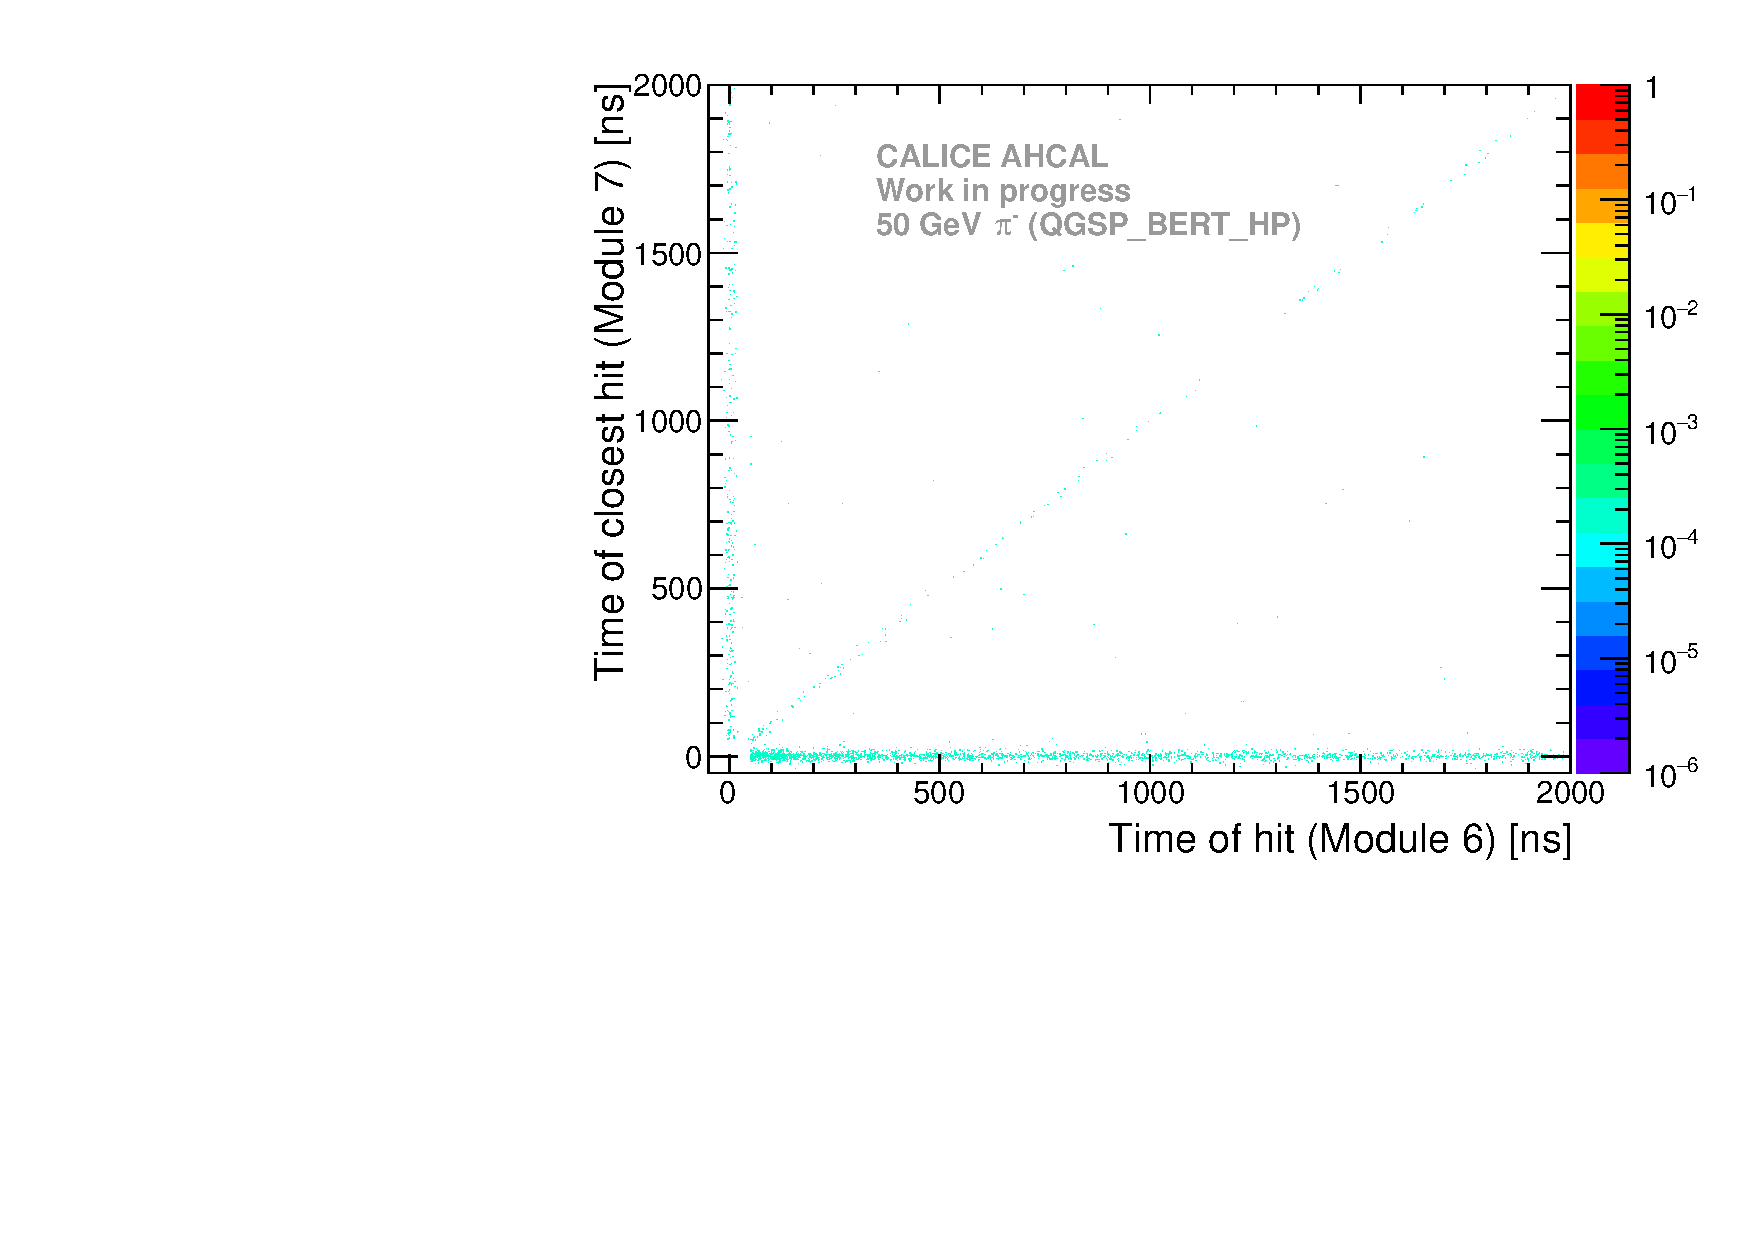
\includegraphics[width=1\textwidth]{../Thesis_Plots/Timing/Pions/Plots/ComparisonToSim/Time_Correlation_50GeV_short_QGSPBERTHP.pdf}
		\caption{Short correlation (QGSP\_BERT\_HP).} \label{fig:Corr_short_QGSPBERTHP}
	\end{subfigure}
	\hfill
	\begin{subfigure}[t]{0.5\textwidth}
		\centering
		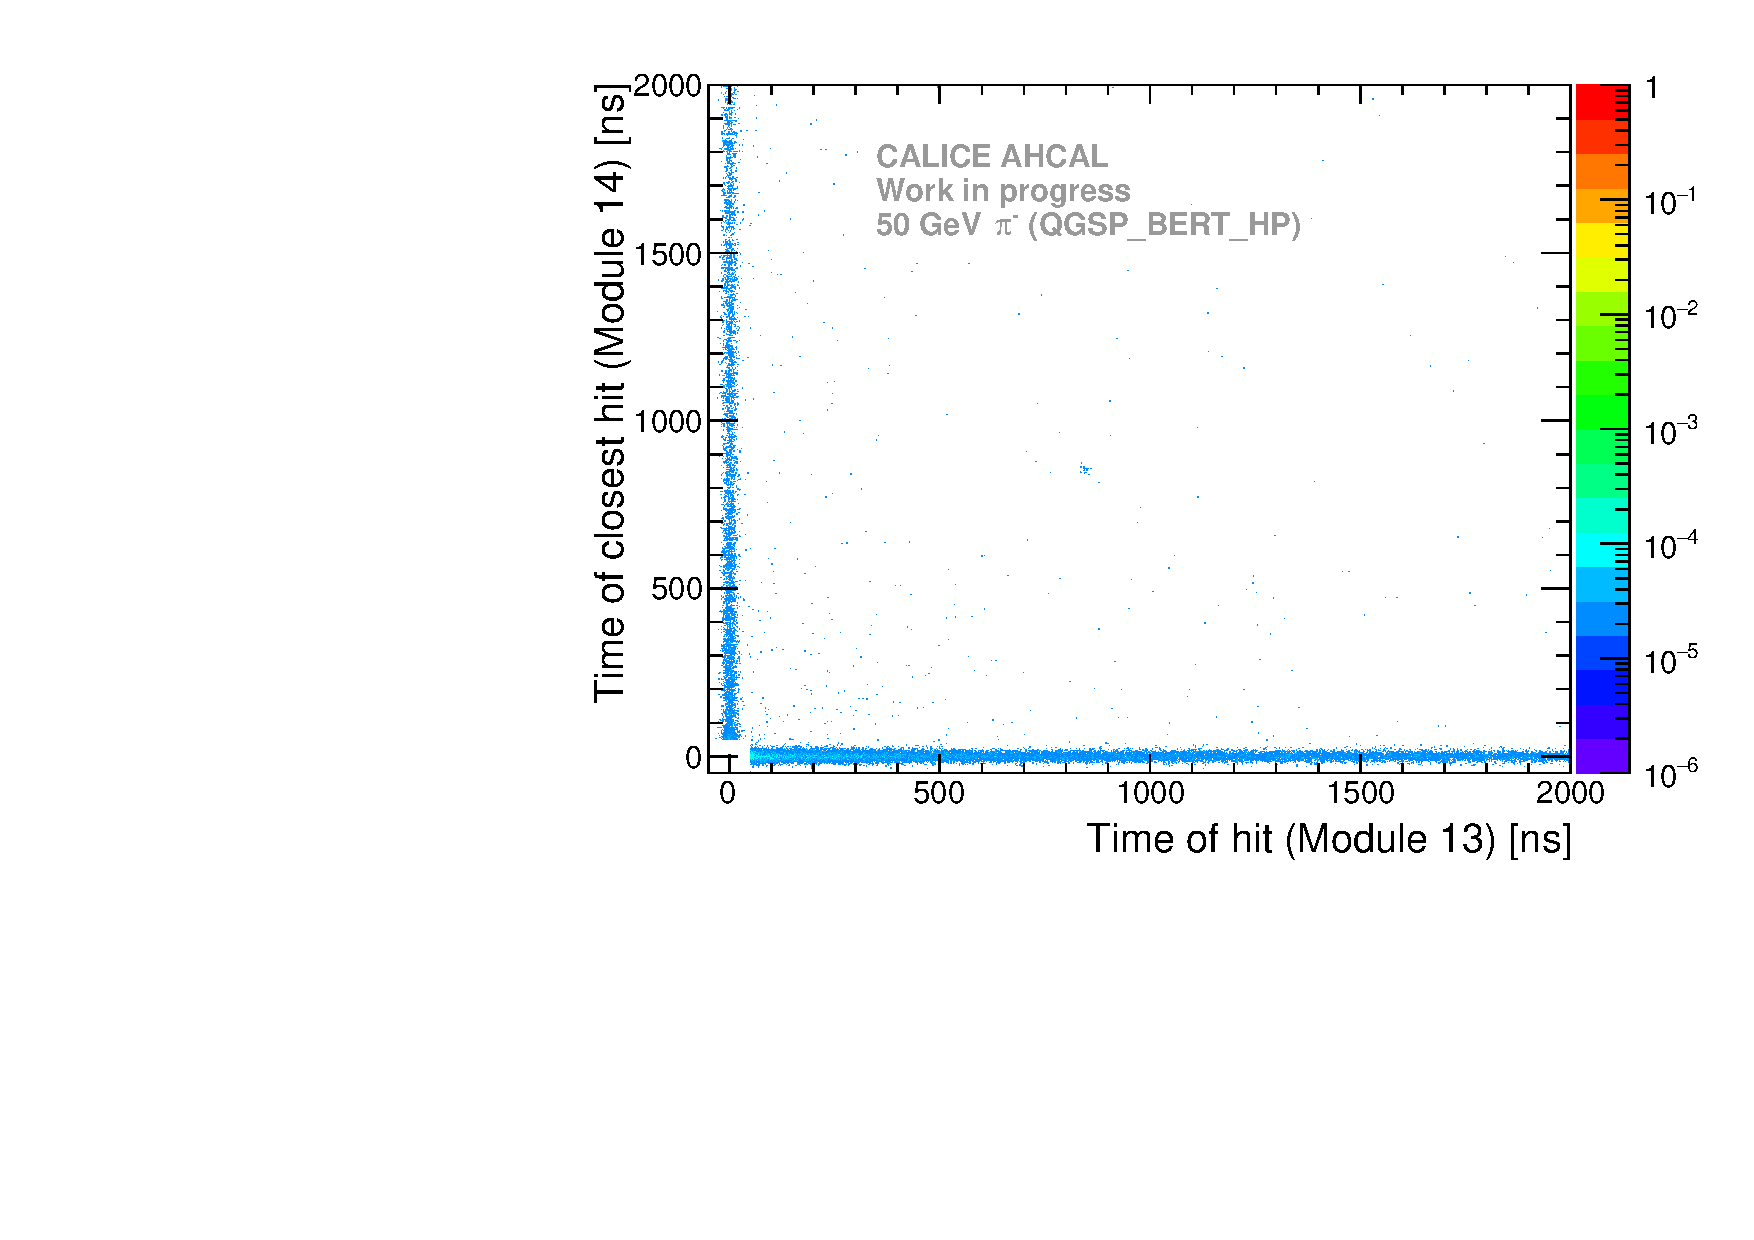
\includegraphics[width=1\textwidth]{../Thesis_Plots/Timing/Pions/Plots/ComparisonToSim/Time_Correlation_50GeV_long_QGSPBERTHP.pdf}
		\caption{Long correlation (QGSP\_BERT\_HP).} \label{fig:Corr_long_QGSPBERTHP}
	\end{subfigure}
	\hfill
	\begin{subfigure}[t]{0.5\textwidth}
		\centering
		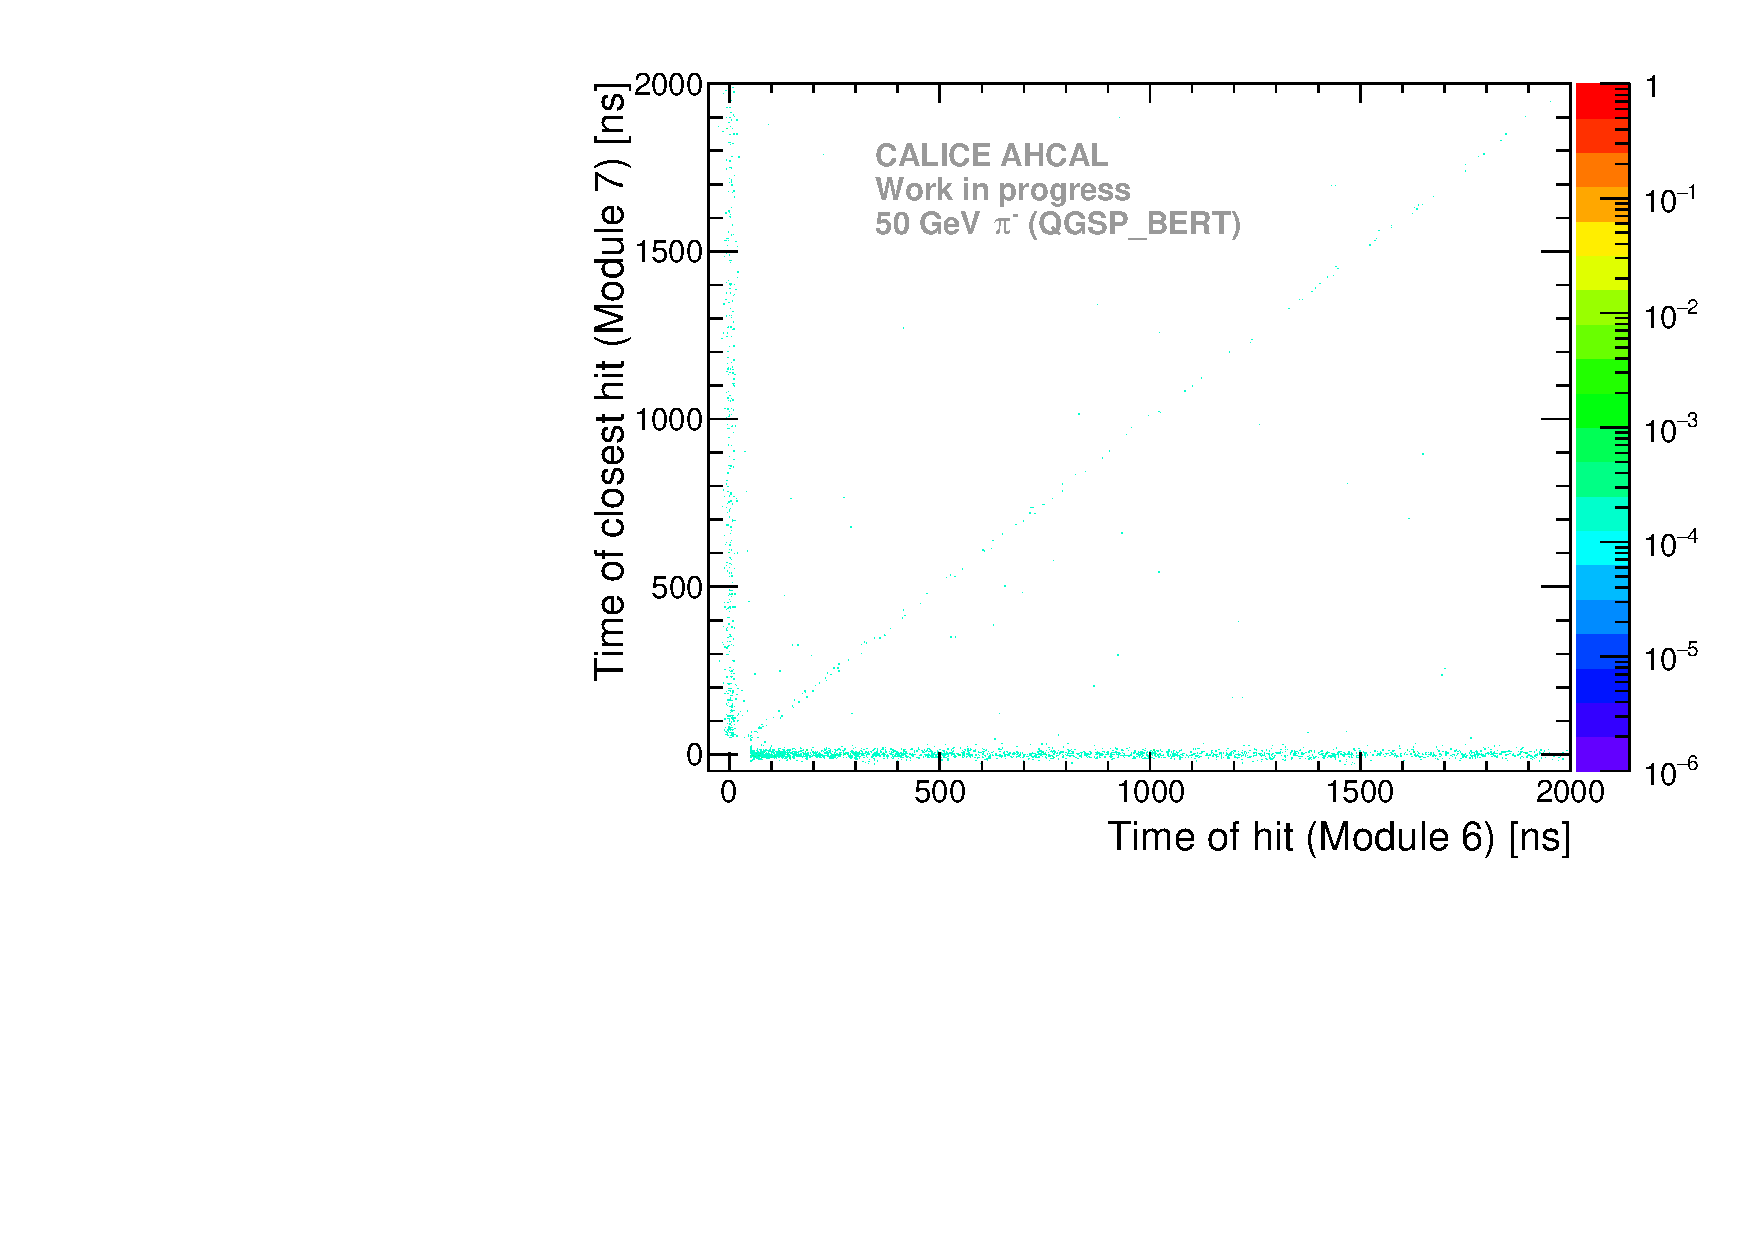
\includegraphics[width=1\textwidth]{../Thesis_Plots/Timing/Pions/Plots/ComparisonToSim/Time_Correlation_50GeV_short_QGSPBERT.pdf}
		\caption{Short correlation (QGSP\_BERT).}\label{fig:Corr_short_QGSPBERT}
	\end{subfigure}
	\hfill
	\begin{subfigure}[t]{0.5\textwidth}
		\centering
		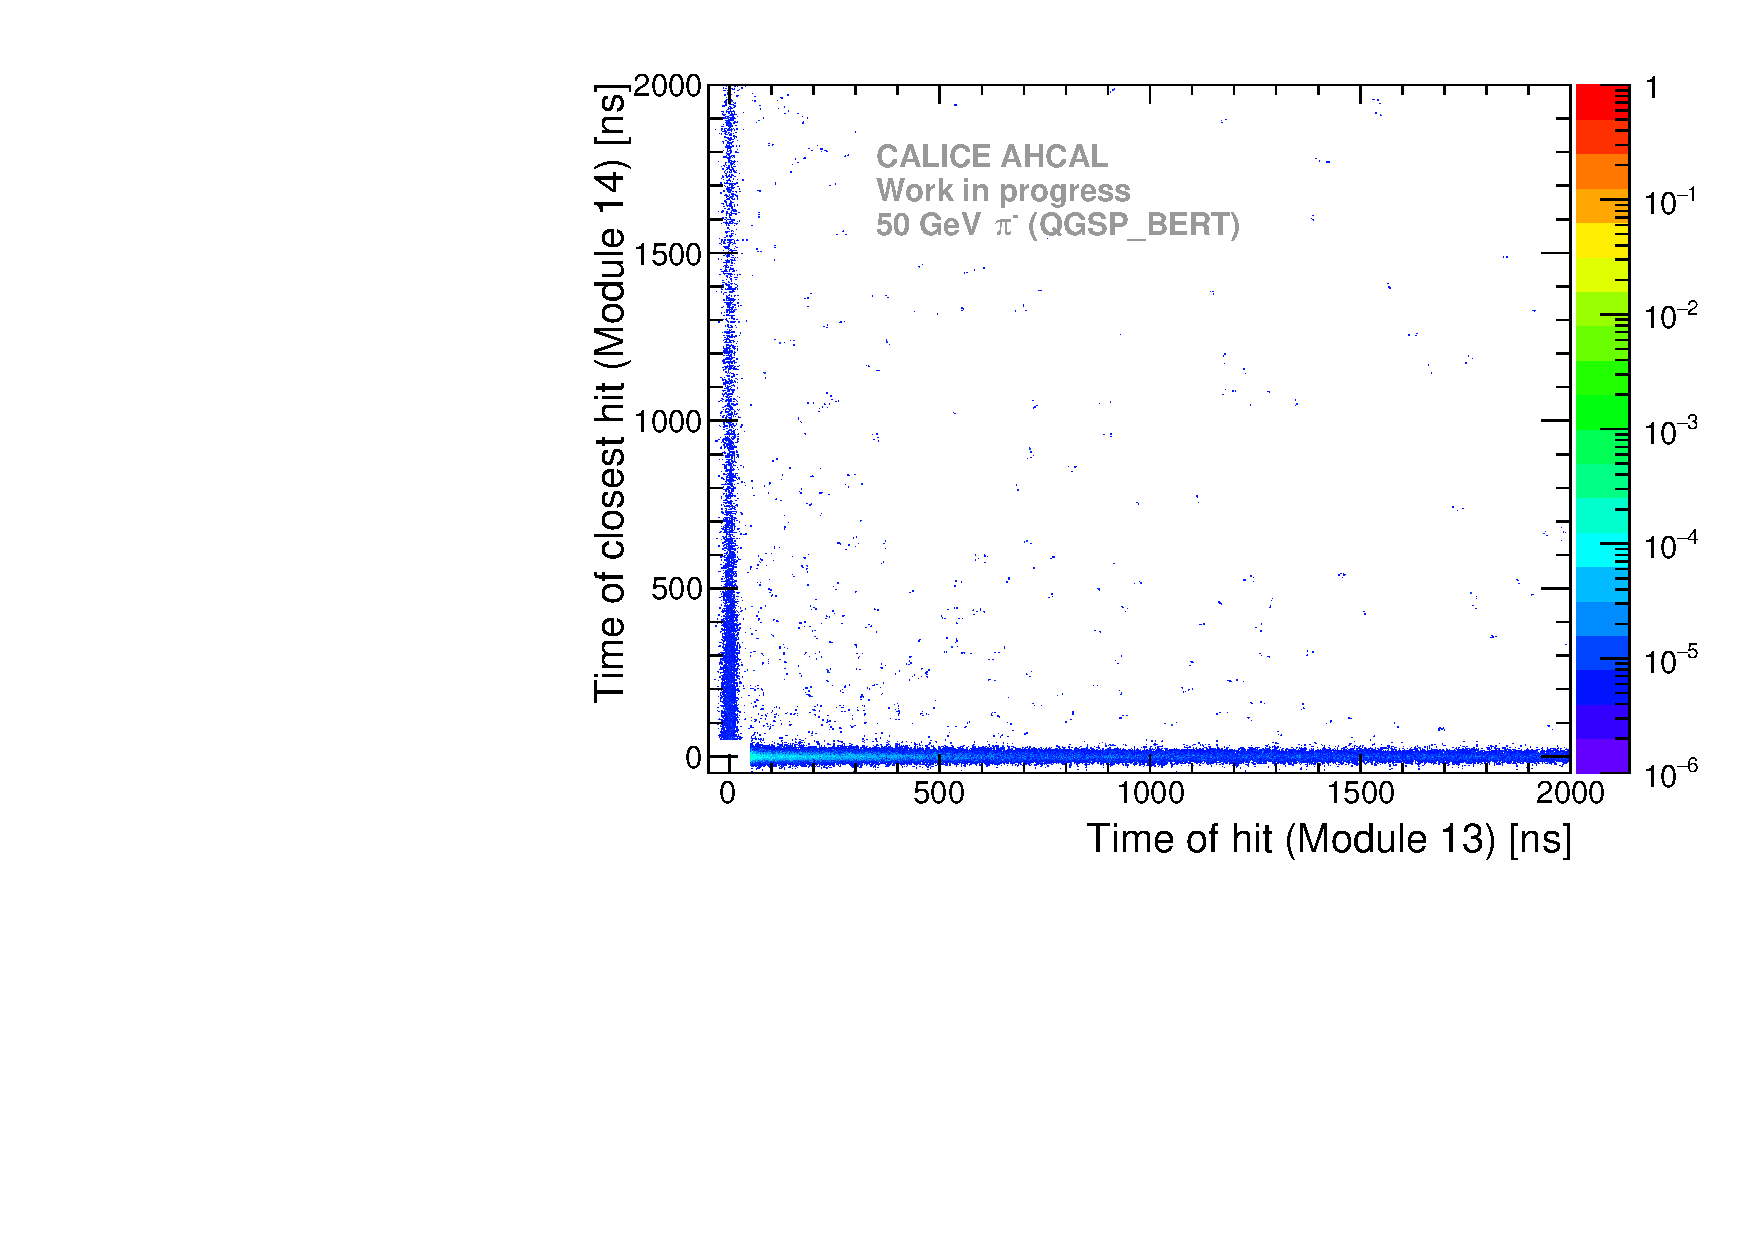
\includegraphics[width=1\textwidth]{../Thesis_Plots/Timing/Pions/Plots/ComparisonToSim/Time_Correlation_50GeV_long_QGSPBERT.pdf}
		\caption{Long correlation (QGSP\_BERT).} \label{fig:Corr_long_QGSPBERT}
	\end{subfigure}
	\hfill
	\begin{subfigure}[t]{0.5\textwidth}
		\centering
		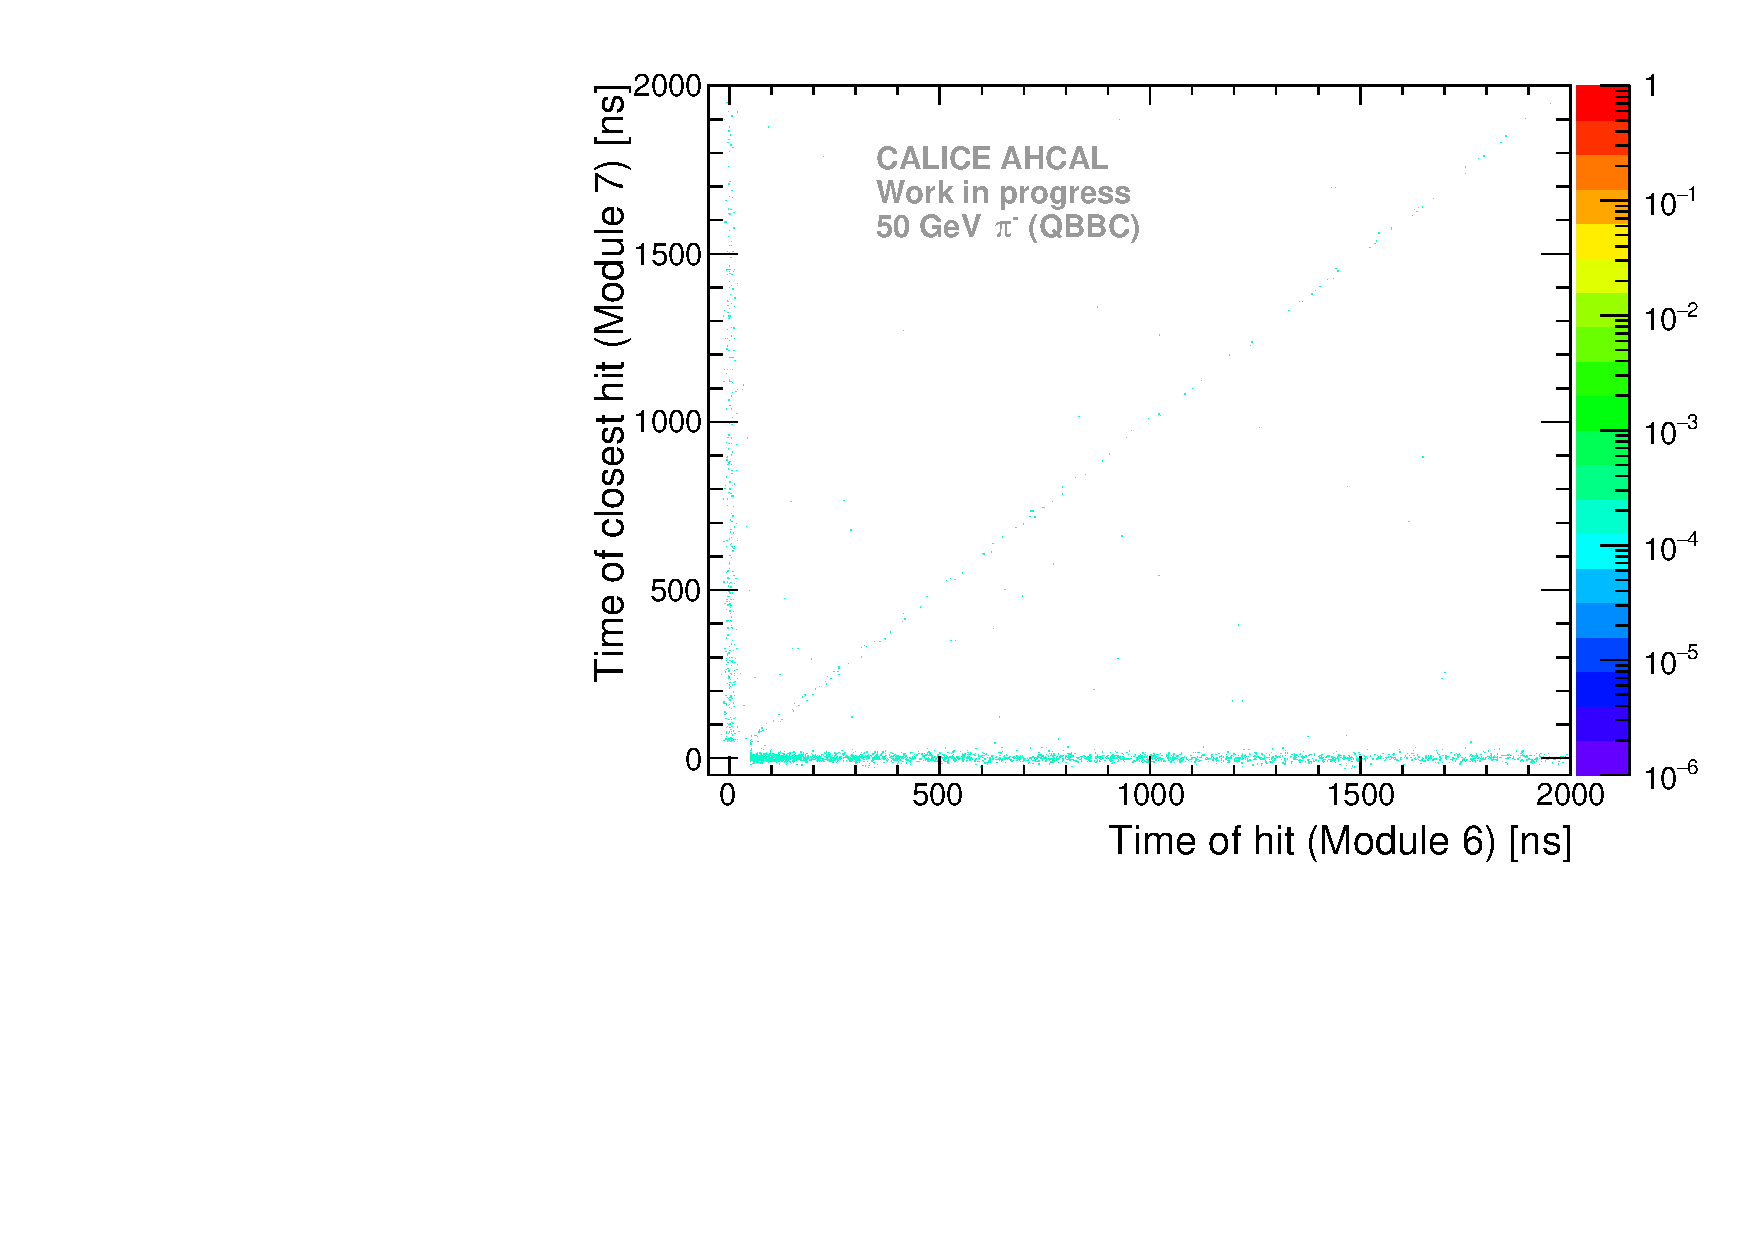
\includegraphics[width=1\textwidth]{../Thesis_Plots/Timing/Pions/Plots/ComparisonToSim/Time_Correlation_50GeV_short_QBBC.pdf}
		\caption{Short correlation (QBBC).} \label{fig:Corr_short_QBBC}
	\end{subfigure}
	\hfill
	\begin{subfigure}[t]{0.5\textwidth}
		\centering
		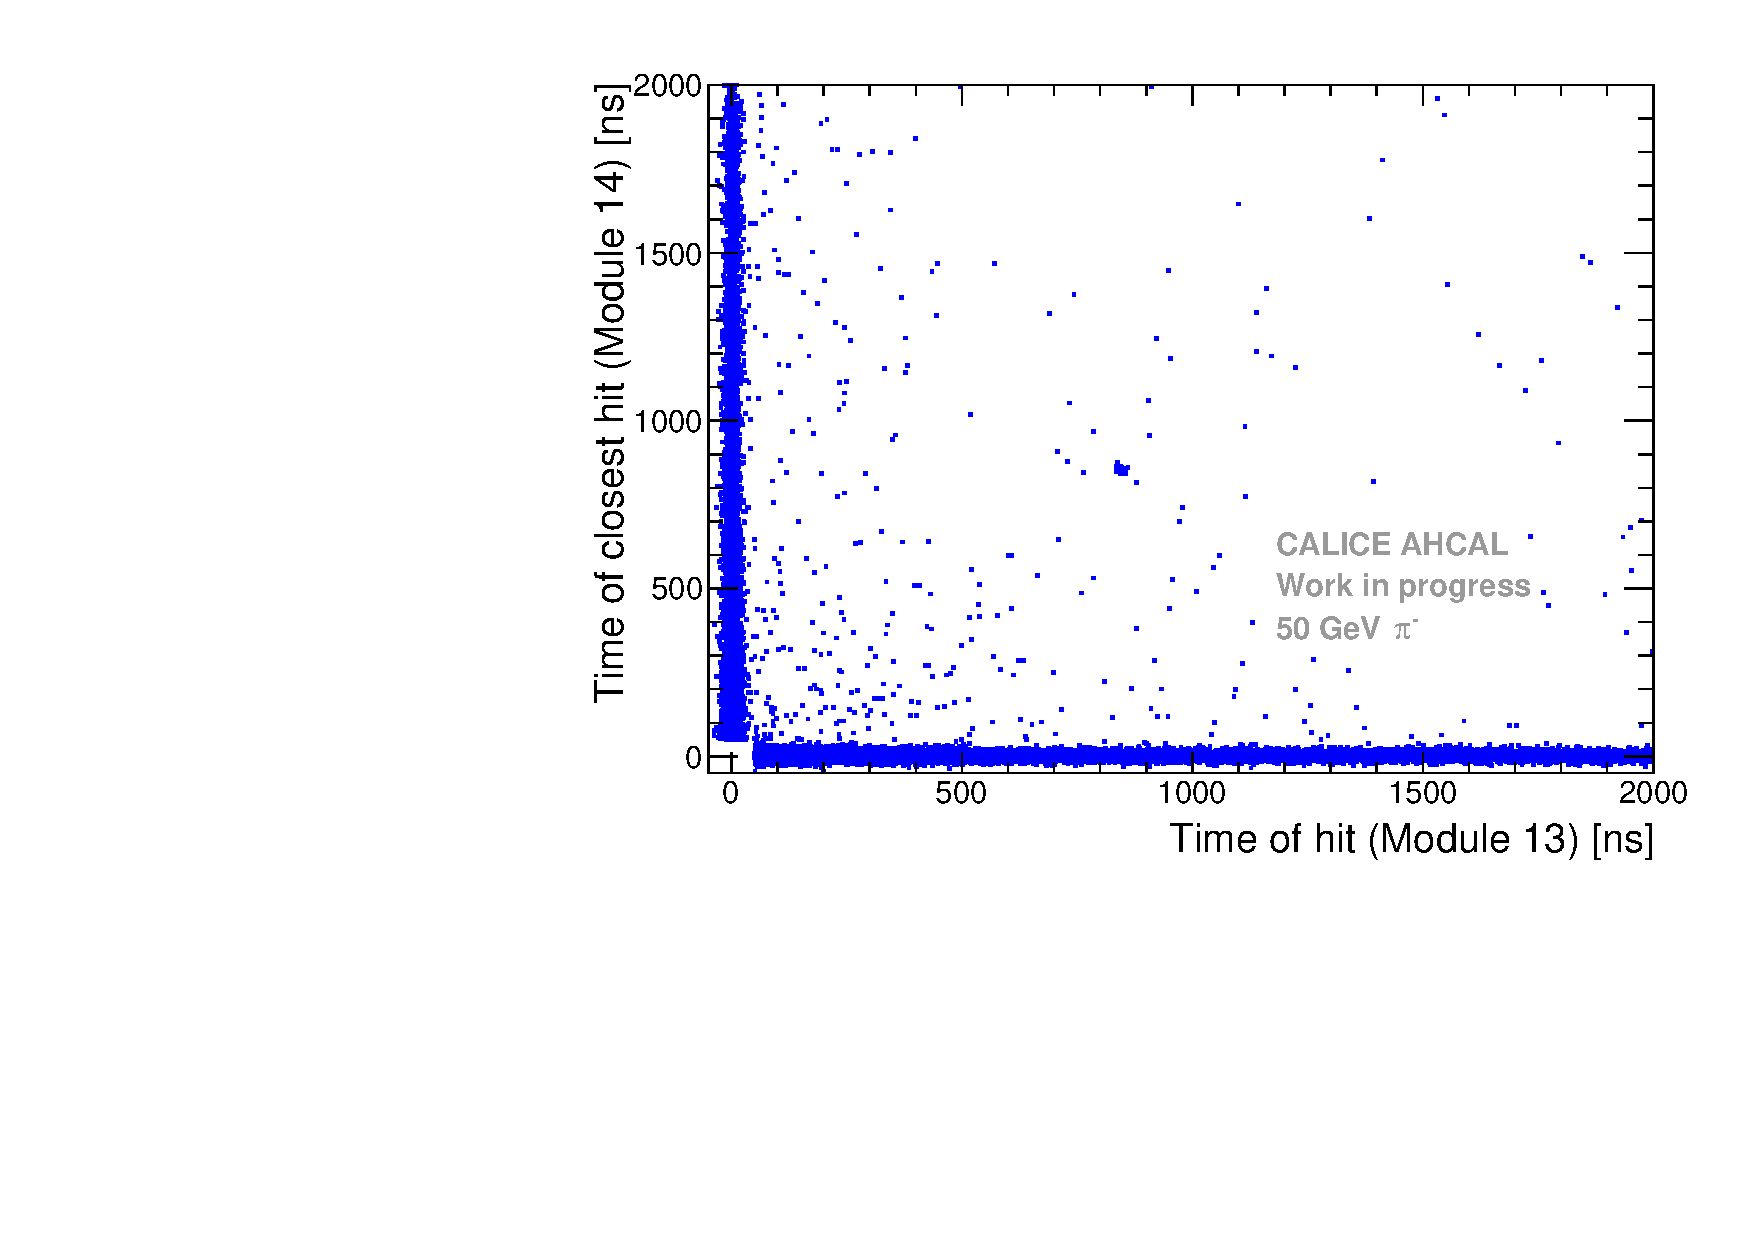
\includegraphics[width=1\textwidth]{../Thesis_Plots/Timing/Pions/Plots/ComparisonToSim/Time_Correlation_50GeV_long_QBBC.pdf}
		\caption{Long correlation (QBBC).} \label{fig:Corr_long_QBBC}
	\end{subfigure}
	\caption{Timing correlations between layers 6 and 7 and layers 13 and 14 in \mokka simulations for different physics lists in 50 GeV pion beam. Each bins are normalized to the number of entries in the 2D histogram.}
	\label{fig:Corr_Mokka_Simulation}
\end{figure}

\section{Comparison of pion showers in a tungsten absorber}

A dataset of pion showers was measured in a tungsten stack in August 2015. The same timing analysis was performed on this dataset \cite{ChristianTungsten} in order to compare pion showers in different stacks and compare the influence of the absorber material on the time development of the shower.

The absolute timing distribution for steel and tungsten absorber is shown in figure \ref{fig:dNdt_ComparisonST}. One can notice that the core of both distributions are very similar, only the intermediate and late components are differing. From around 30 to 80 ns, the fraction of hits between absorbers varies between a factor of 2 to 8. Above 100 ns, the tail flattens and the difference of the fraction of hits is around a factor 10. This shows that in tungsten, the fraction of late hits is greatly increased due to the nature of the tungsten (high Z atom) that increase the fraction of late neutrons produced.

\begin{figure}[htbp!]
	\begin{subfigure}[t]{0.5\textwidth}
		\centering
		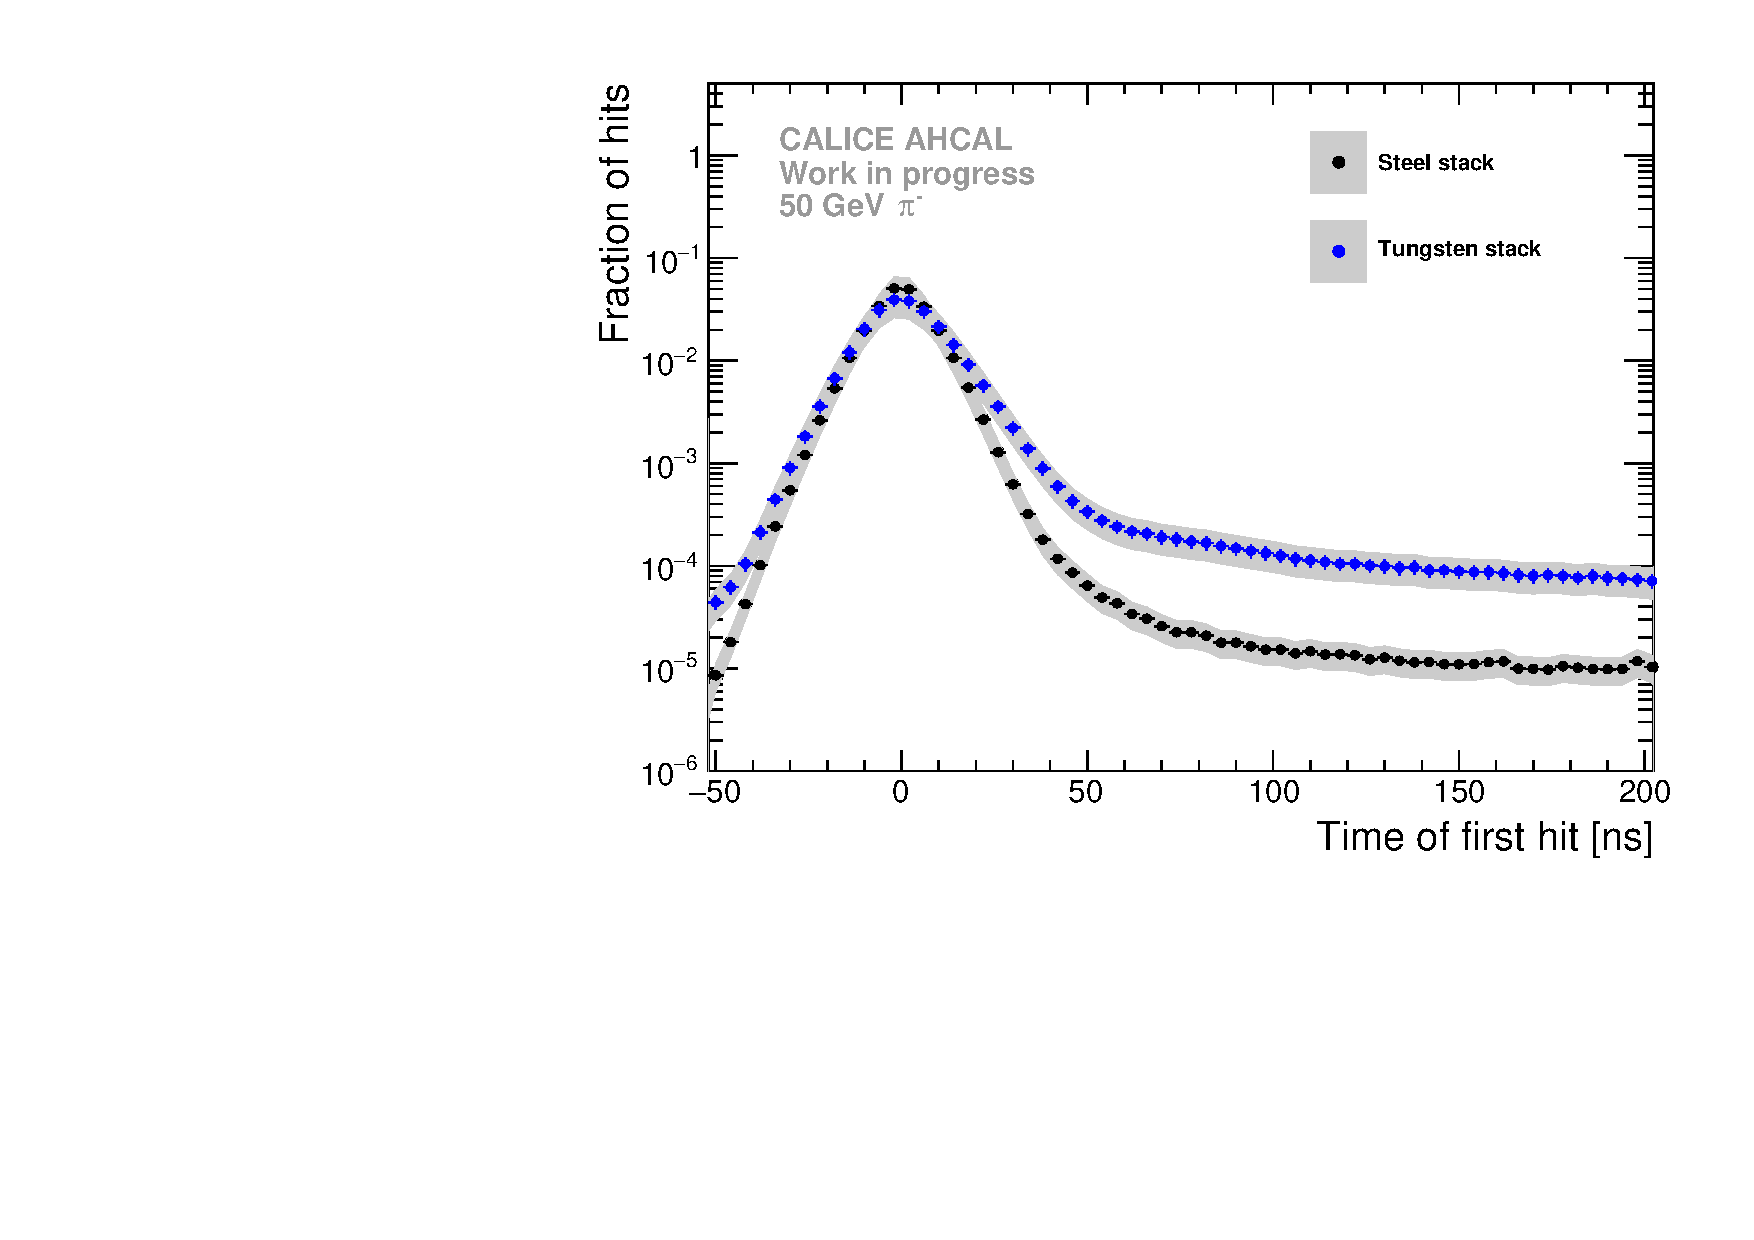
\includegraphics[width=1\textwidth]{../Thesis_Plots/Timing/Pions/Plots/ComparisondNdt_SteelTungsten.pdf}
		\caption{Time correlation between layer 6 and 7 for 50 GeV pions.} \label{fig:dNdt_ComparisonST}
	\end{subfigure}
	\hfill
	\begin{subfigure}[t]{0.5\textwidth}
		\centering
		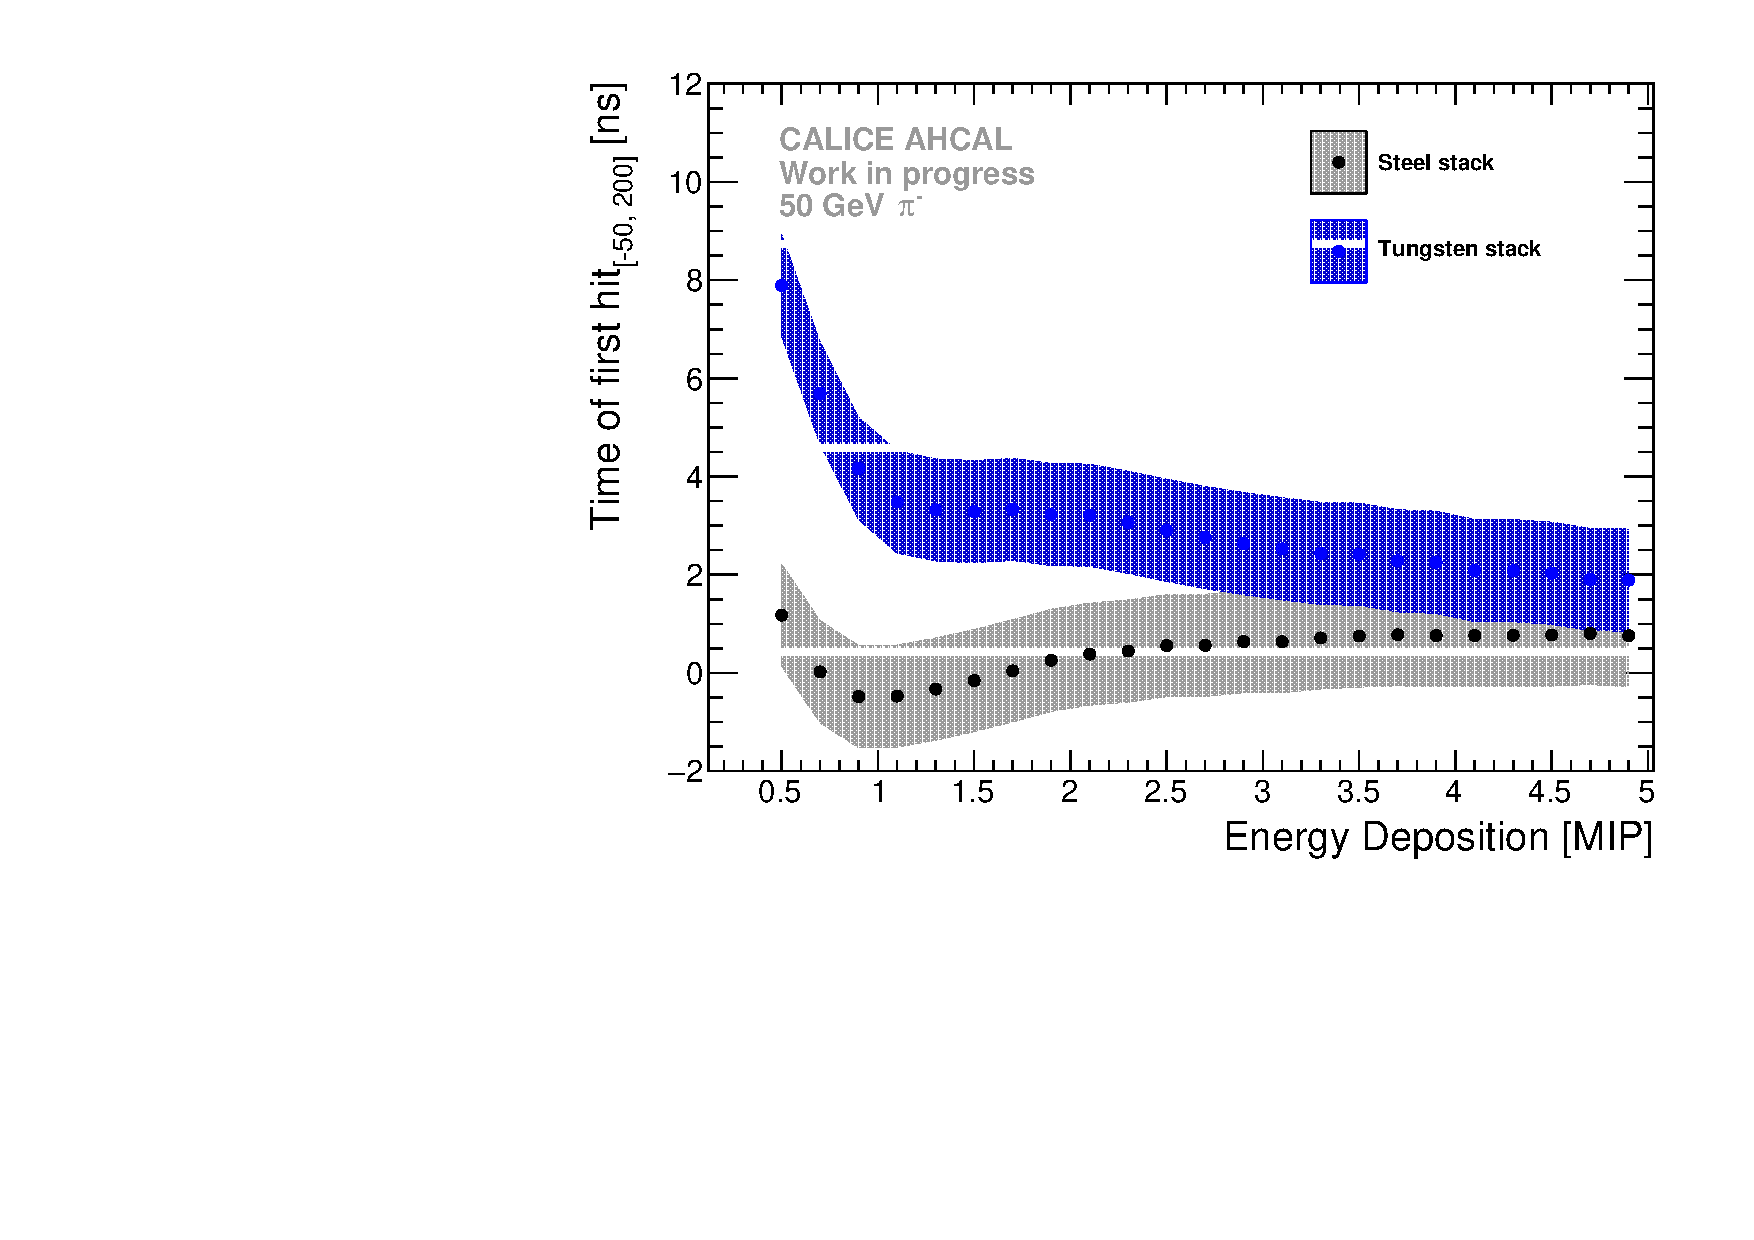
\includegraphics[width=1\textwidth]{../Thesis_Plots/Timing/Pions/Plots/ComparisonEnergy_SteelTungsten.pdf}
		\caption{Time correlation between layer 13 and 14 for 50 GeV pions.}\label{fig:Energy_ComparisonST}
	\end{subfigure}
	\caption{On the left, distribution of the time of first hit for 50 GeV pions in steel (black) and tungsten (blue) absorbers in a range of -50 to 200 ns. On the right, the time of first hit as function of the hit energy for 50 GeV pions in steel (black) and tungsten (blue) absorbers in a range of -50 to 200 ns. The bands represent the systematic uncertainty.}
\end{figure}

The mean time of the first hit as function of the hit energy is shown in figure \ref{fig:Energy_ComparisonST}. One can observe that the delayed time component from low energy neutrons is significantly enhanced in tungsten absorber. At 0.5 MIP, a factor of around 8 is observed. Also, the decrease of the time is not as fast as in steel absorber where at around 1 MIP, a delay of around 4 ns is seen and goes slowly down as function of the hit energy. Finally, the mean time of the first hit as function of the hit distance to the center of gravity in the $x:y$ plane is shown in figure \ref{fig:Radius_ComparisonST}. In the first few tiles (up to 60 mm), the time of first hit is very similar in tungsten and steel. As the hit is far away from the center of gravity, the difference in time increase between steel and tungsten. In tungsten, the time of first hit is much more delayed than in steel by a factor around 8-10. This confirms further that the delayed component coming from low energy neutrons is spread at high distance to the shower core.

\begin{figure}[htbp!]
	\centering
	\includegraphics[width=0.6\textwidth]{../Thesis_Plots/Timing/Pions/Plots/ComparisonRadius_SteelTungsten.pdf}
	\caption{Time of first hit as function of the hit distance to the CoG in $x:y$ plane for 50 GeV pions in steel (black) and tungsten (blue) absorbers in a range of -50 to 200 ns. The bands represent the systematic uncertainty.}
	\label{fig:Radius_ComparisonST}
\end{figure}

\section{Summary and Outlook}

The understanding of the time structure of hadronic showers and the level of accuracy reflected in \geant simulations is highly relevant for calorimeters at future (linear) collider experiments. This can be applied for conditions with high level of background such as $\gamma\gamma \rightarrow hadrons$ or high repetition rates experiments to remove out-of-time pile-up events.

The AHCAL testbeam at CERN in July 2015 was focused to address this, with steel absorber and close to the ILD detector design, by collecting data from muon, electron and pion beams. The AHCAL technological prototype was equipped with 14 layers using scintillator tiles as active material readout by SiPMs to provide radial and longitudinal sampling of showers with high granularity and ns-scale time resolution. For the first time, time study of hadronic showers was done on a large scale using integrated readout electronics.
In this analysis, the time calibration procedure of the AHCAL was presented. A time resolution of the order of 5 ns is achieved for a muon beam. Due to an effect of the readout electronics, the time resolution for electron and pion beams is worse, with a value of 8 ns.

Studying hadronic showers, the data shows that late depositions are concentrated at low hit energies below 1.5 MIPs in iron. These hits are mostly at a great distance from the shower axis, while the electromagnetic sub-showers and relativistic hadrons are predominant near the shower axis. Timing correlations between layers have also been investigated. Correlations are visible at short range as well as long range in different proportions in the data.

The comparison of detailed simulations with data has been performed. It shows that in general, the simulation reproduces well the data within the systematics. The tracking of low energy neutrons in the HP package or other implementations like in QBBC show that they are needed to reproduce well the tail of the data which is otherwise generally over-estimated. Time correlations are reproduced in simulation but the proportion of hits in data and simulation differ quite significantly. This may be due to the selection of the data that does not reject efficiently multi-particle events and would need more data and investigations to understand their origin.

The running mode in Testbeam does not reflect the time resolution that would be accessible in ILC running mode. By extrapolation, assuming that the time resolution scales linearly with the frequency of the slow clock, a time resolution of the order of 1 ns would be obtained. The use of timing information could be a powerful tool to have to help in separating nearby showers in case of very busy events, for example a $ttH$ event. It could be used in a software compensation way by using timing bins differentiating electromagnetic sub-showers or relativistic hadrons and the hadronic late component, and weight them accordingly.
